% TODO: explain branching

\documentclass[a4paper,11pt]{article}
\usepackage{float}
\usepackage{subfig}
\usepackage{fullpage}
\usepackage{booktabs}
\usepackage{tikz}
\usepackage{pgfplots}
\usepackage{pgfplotstable}
%\pgfplotsset{plot coordinates/math parser=false}
\usetikzlibrary{calc}
\pgfplotsset{compat=newest}
%\usetikzlibrary{colorbrewer}
 \usetikzlibrary{
   pgfplots.colorbrewer,
 }
\pgfplotsset{compat=newest}
\usepackage{cwpuzzle}
%\usepackage{algpseudocode}
\usepackage{astra}
%\usepackage{etoolbox}\AtBeginEnvironment{algorithmic}{\small‌​}
%\usepackage{algorithm2e}
%\usepackage{algorithmicx}
%\input{macros}

%\usepackage{amsthm}
\usepackage{amsthm}

\newtheorem{definition}{Definition}
%\newtheorem{proof}{Proof}
\newtheorem{theorem}{Theorem}[section]
\newtheorem{corollary}{Corollary}[theorem]
\newtheorem{lemma}[theorem]{Lemma}

\newcommand{\CT}[0]{CT~}

% Silly but saves space
\newcommand{\T}[1]{\texttt{#1}}

\newcommand{\Timeout}{600.00} % CPU seconds
\newcommand{\Todo}[1]{{\color{blue}#1}}
\newcommand{\Secref}[1]{Section~\ref{#1}}
\newcommand{\Chapref}[1]{Section~\ref{#1}}
\newcommand{\Algoref}[1]{Algorithm~\ref{#1}}
\newcommand{\Table}{\Constraint{Table}}
\newcommand{\Regular}{\Constraint{Regular}}
\newcommand{\Extensional}{\Constraint{Extensional}~}
\newcommand{\Lineref}[1]{Line~\ref{#1}}
\newcommand{\Linesref}[2]{Lines~\ref{#1}--\ref{#2}}
\newcommand{\lineref}[1]{line~\ref{#1}}
\newcommand{\linesref}[2]{lines~\ref{#1}--\ref{#2}}
\newcommand{\Defref}[1]{Definition~\ref{#1}}
\newcommand{\Thmref}[1]{Theorem~\ref{#1}}
\newcommand{\Lemmaref}[1]{Lemma~\ref{#1}}

\newcommand{\Reg}[0]{Reg~}
\newcommand{\Tups}[0]{Tup\_speed~}
\newcommand{\Tupm}[0]{Tup\_mem~}

\newcommand{\Eqref}[1]{\eqref{#1}}

\newcommand{\Method}[2]{\textbf{method~}\mathrm{{#1}}({#2})}
\newcommand{\MethodReturn}[3]{\textbf{method~}\mathrm{{#1}}({#2})\textbf{\ : \ {#3}}}
\newcommand{\Class}{\textbf{Class~}}
\newcommand{\Constructor}{\textbf{constructor~}}

\newcommand{\Dom}[1]{\text{dom}({#1})}
\newcommand{\Dominit}[1]{\underline{\text{dom}}(#1)}


%\newcommand{\Ceiling}[1]{\left\lceil#1\right\rceil}
%\newcommand{\Floor}[1]{\left\lfloor#1\right\rfloor}


% SparseBitSet
\newcommand{\Words}{\texttt{words}}
\newcommand{\Index}{\texttt{currToOrig}}
\newcommand{\Mask}{\texttt{mask}}
\newcommand{\Limit}{\texttt{limit}}
\newcommand{\SparseBitSet}{\texttt{SparseBitSet}}
\newcommand{\Offset}{\localvar{offset}}

% CT Propagator
\newcommand{\Scp}{\texttt{vars}}
\newcommand{\CurrTable}{\texttt{validTuples}}
\newcommand{\Sval}{\texttt{S^{val}}}
\newcommand{\Ssup}{\texttt{S^{sup}}}
\newcommand{\LastSizes}{\texttt{lastSize}}
\newcommand{\Supports}{\texttt{supports}}
\newcommand{\Residues}{\texttt{residues}}
\newcommand{\Vars}{\texttt{vars}}

% Pseduo code
\newcommand{\ForEach}[1]{\textbf{foreach } {#1} \textbf{ do }}
\newcommand{\ForEachTo}[3]{\textbf{foreach } {#1} \textbf{ from } {#2} 
  \textbf{ to } {#3} \textbf{ do }}
\newcommand{\ForEachDownTo}[3]{\textbf{foreach } {#1} \textbf{ from } {#2} 
  \textbf{ downto } {#3} \textbf{ do }}
\newcommand{\Break}{\textbf{break~}}
\newcommand{\While}[1]{\textbf{while~} {#1} \textbf{~do~}}

\renewcommand{\algorithmicfor}{\textbf{Method}}
\renewcommand{\algorithmicdo}{}
\renewcommand{\algorithmicforall}{\textbf{foreach}}
%\renewcommand{\algorithmicwhile}{\textbf{foreach}}

\newcommand{\Func}[2]{\FOR{#1(#2)}}
\newcommand{\FuncRet}[3]{\FOR{#1(#2) \ : \ \textbf{#3}}}
\newcommand{\Endfunc}{\ENDFOR}
\newcommand{\To}{~\bf{to}~}
\newcommand{\Downto}{~{\bf{downto}}~}
%\newcommand{\For}[3]{\FOREACH{${#1} \leftarrow {#2} \To {#3}$}}

\newcommand{\FOREACH}[1]{\FORALL{{#1} \textbf{do}}}
\newcommand{\ENDFOREACH}{\ENDFOR}

\newcommand{\For}[3]{\STATE \textbf{for} ${#1} \leftarrow {#2} \To {#3}$ \textbf{do} \begin{ALC@g}}
\newcommand{\ForDown}[3]{\STATE \textbf{for} ${#1} \leftarrow {#2} \Downto {#3}$ \textbf{do} \begin{ALC@g}}
\newcommand{\EndFor}{\end{ALC@g}}

\renewcommand{\algorithmiccomment}[1]{\hfill // #1}
\def\PROCEDURE{\item[\textbf{PROCEDURE}]}
\def\FAILED{\textbf{FAILED}}
\def\NOFIX{\textbf{NOFIX}}
\def\FIX{\textbf{FIX}}
\def\SUBSUMED{\textbf{SUBSUMED}}
\def\FAIL{\textbf{FAIL}}
\def\bool{\mathit{bool}}
\def\StatusMessage{\mathit{StatusMessage}}
\def\FindSupport{\textsc{FindSupport}}
\def\RemoveSupport{\textsc{RemoveSupport}}
\def\Extensional{\textsc{Extensional}}
\def\CompactTable{\textsc{CompactTable}}
\def\UpdateTable{\textsc{UpdateTable}}
\def\FilterDomains{\textsc{FilterDomains}}
\def\FixDomains{\textsc{FixDomains}}
\def\InitialiseCT{\textsc{InitialiseCT}}
\def\IndexOfFixed{\mathit{index\_of\_fixed}}


\newcommand{\ITE}[3]{\text{\bf ~if~} #1 \text{\bf ~then~} #2 \text{\bf ~else~} #3 \text{\bf ~endif}}

\newcommand{\function}[1]{\mathrm{#1}}
\newcommand{\localvar}[1]{\mathit{#1}}

\newlength\myindent
\setlength\myindent{2em}
\newcommand\bindent{%
  \begingroup
  \setlength{\itemindent}{\myindent}
  \addtolength{\algorithmicindent}{\myindent}
}
\newcommand\eindent{\endgroup}

\newcommand{\INDSTATE}[1][1]{\STATE\hspace{#1\algorithmicindent}}
\newcommand{\INDRETURN}[1][1]{\STATE\hspace{#1\algorithmicindent}\textbf{return~}}
\newcommand{\INDIF}[2][1]{\STATE\hspace{#1\algorithmicindent}
  \textbf{if~}{#2}\textbf{~then}}
\newcommand{\INDELSE}[1][1]{\STATE\hspace{#1\algorithmicindent}\textbf{else~}}
\newcommand{\INDELSEIF}[2][1]{\STATE\hspace{#1\algorithmicindent}
  \textbf{else if~}{#2}\textbf{~then}}

\newcommand{\CTpaper}[0]{DBLP:conf/cp/DemeulenaereHLP16}

\numberwithin{equation}{section}

\title{\textbf{Implementation and Evaluation of a\\
    Compact-Table Propagator in Gecode
  }
}

\author{Linnea Ingmar} % replace by your name(s)

%\date{Month Day, Year}
\date{\today}

\begin{document}

\maketitle

\tableofcontents

\newpage

\section{Introduction}
\label{intro}

% What is CP?
% What is a propagator?
% Gecode
% Goal

Constraint programming (CP)~\cite{Apt:constraintsBook}
is a programming paradigm that is used for solving
combinatorial problems. Within the paradigm, a problem is
modelled as a set of \emph{constraints} on a
set of \emph{variables} that each can take on a number of
possible values. The possible values of 
a variable form what is called the \emph{domain} of the variable.
A \emph{solution} to a constraint problem must assign all variables
a value from their domains, so that all the constraints of the problem
are satisfied. Additionally, in some cases the solution should not only
satisfy the set of constraints for the
problem, but also maximise or minimise some given function on the variables.


%A constraint solver (CP solver) is a software that solves constraint problems.
A solution to a constraint problem is found by generating a search
tree, branching on partitions of the possible values for the variables. 
At each node in the search tree, conflicting values are filtered out
from the domains of the variables in a process called~\emph{propagation},
effectively reducing the size of the search tree.
Each constraint is associated with a \emph{propagation algorithm},
called a~\emph{propagator},
that implements the propagation for that constraint by removing
values from the domains that are in conflict with the constraint.

The \Table~constraint expresses the possible combinations of values
that the associated variables can take as a set of tuples.
Assuming finite domains, the \Table~constraint can theoretically
encode any kind of constraint and is thus very powerful. 
The design of propagation algorithms for \Table~is an active research field,
and several algorithms are known. In 2016, a new propagation algorithm for the
\Table~constraint was published~\cite{\CTpaper}, called Compact-Table (CT).
The results published in the named paper indicate that CT outperforms all previously
known algorithms in terms of runtime.

A constraint programming solver (CP solver) is a software that solves constraint problems.
\emph{Gecode}~\cite{Gecode} is a popular CP solver written in C++ that combines
state-of-the-art performance with modularity and extensibility.
Presently, Gecode has two existing propagators for~\Table,
but to the best of my knowledge there have been no attempts to implement
CT in Gecode before this project.
Consequently, its performance in Gecode was unknown. 
The purpose of this thesis is therefore to implement CT in Gecode and to evaluate
and compare its performance with the existing propagators for
the \Table~constraint.
The results of the evaluation indicate that CT outperforms
the existing propagation algorithms in Gecode for \Table,
which suggests that CT should be included in the solver.

% In Constraint Programming (CP), every constraint is associated with a propagator
% algorithm. The propagator algorithm filters out impossible values for the variables
% related to the constraint. For the \Table~constraint, several propagator
% algorithms are known. In 2016, a new propagator algorithm for the \Table
% constraint was published~\cite{\CTpaper}, called Compact-Table (CT).
% Preliminary results indicate that CT outperforms the previously known algorithms.
% There has been no attempt to implement CT in the constraint solver Gecode~\cite{Gecode}, 
% and consequently its performance in Gecode is unknown.

\subsection{Goal}
\label{intro:goal}
The goal of this bachelor's thesis is the design, documentation and implementation
of a CT propagator algorithm for the \Table~constraint in Gecode,
and the evaluation of its performance compared to the existing propagators.

\subsection{Contributions}
\label{intro:contributions}

The following items are the contributions made by this dissertation,
while simultaneously serving as a description of the outline:

\begin{itemize}
  \item The preliminaries that are relevant for the rest of the dissertation
    are covered in \Secref{bg}.

  \item The algorithms presented in the paper that is the starting point of this 
    project~\cite{DBLP:conf/cp/DemeulenaereHLP16} 
    have been modified to suit the target CP solver Gecode, and are presented and explained in 
    \Secref{sec:algorithms}.

  \item Several versions of the CT algorithm have been implemented in Gecode, and
    the implementation is discussed in \Secref{sec:implementation}.

  \item The performance of the CT algorithm has been evaluated,
    and the results
    are presented and discussed in \Secref{evaluation}.

  \item The conclusion of the project is that the results indicate
    that CT outperforms the existing propagation algorithms of Gecode, which
    suggests that CT should be included in Gecode; this is discussed
    in \Secref{conclusions}.

  \item Several possible improvements and flaws have been detected in the current
    implementation that need to be fixed for the code to reach production 
    quality; these are listed in \Secref{conclusions}.
        
\end{itemize}

\section{Background}
\label{bg}

% Definiera alla begrepp som används senare

This section provides a background that is relevant for the
following sections. It is divided into five parts: \Secref{bg:cp}
introduces Constraint Programming. \Secref{bg:propagation} discusses
the concepts propagation and propagators in detail.
\Secref{bg:gecode} gives an overview
of Gecode, a constraint programming solver.
\Secref{bg:table} introduces the~\Table~constraint.
\Secref{bg:ct} describes the main concepts of the 
Compact-Table (CT) propagation algorithm.
Finally, \Secref{bg:sbs} 
describes the main idea of reversible sparse bit-sets,
a data structure that is used in the CT algorithm.

\subsection{Constraint Programming}
\label{bg:cp}
Constraint programming (CP)~\cite{Apt:constraintsBook}
is a programming paradigm that is used for solving
combinatorial problems. Within the paradigm, a problem is
modelled as a set of \emph{constraints} on a
set of \emph{variables} that each can take on a number of
possible values. The possible values of 
a variable form what is called the \emph{domain} of the variable.
A \emph{solution} to a constraint problem must assign all variables
a value from their domains, so that all the constraints of the problem
are satisfied. Additionally, in some cases the solution should not only
satisfy the set of constraints for the
problem, but also maximise or minimise some given function on the variables.

A constraint programming solver (CP solver) is a software that
takes constraint problems expressed in some modelling language as input,
tries to solve them, and outputs the results to the user of the software.
The process of solving a problem consists of generating a search tree by branching
on partitions of the possible values for the variables. 
At each node in the search tree,
the solver removes impossible values from the domains of variables.
This filtering process is called \emph{propagation}. Each constraint is
associated with at least one propagation algorithm, whose purpose is to detect
and remove values from the domains of the variables
that cannot participate in a solution because assigning them to
the variables would violate the constraint,
effectively shrinking the domain sizes and thus 
pruning the search tree.
When sufficient\footnote{Here ``sufficient'' might either mean that no more
  propagation can be made, or that more propagation is possible,
  but the solver has decided that it is more efficient to branch to a new node instead of 
  performing more propagation at the current node.}
propagation has been performed and a solution is still not found,
the solver must \emph{branch} the search tree, following some heuristic,
which typically involves selecting a variable and partitioning its domain 
into a number of subsets, creating as many branches as subsets.
Each subset is associated with one branch, along which the domain
of the variable is restricted to that subset.
When search moves to a new node in the tree propagation starts over again.

Propagation interleaved with branching continues along a path in the search tree,
until the search reaches a leaf node, which can be either a
\emph{solution node} or a \emph{failed node}.
In a solution node a solution to the problem is found:
all variables are assigned a value
from their domains, and all the constraints are satisfied.
In a failed node, the domain of a variable has become empty, which
means that a solution could not be found along that path.
From a failed node, search must backtrack and continue from a node where all branches
have not been tried yet. If all leaves of the tree consist of failed nodes, then
the problem is unsatisfiable, else there is a solution that will be
found if search is allowed to go on long enough.

To build intuition and understanding of the ideas of CP,
the concepts can be illustrated with logical puzzles. One such
puzzle is Kakuro, somewhat similar to the popular puzzle Sudoku,
a kind of mathematical crossword where the ``words'' consist
of numbers instead of letters, see Figure~\ref{fig:kakuro}.
The game board consists of 
blank white cells forming rows and columns, called \emph{entries}.
Each entry has a \emph{clue}, a prefilled number indicating the sum of that entry.
The objective is to put digits from 1 to 9 inclusive into each cell such 
that for each entry,
the sum of all the digits in the entry is equal to the clue of that entry,
and such that each digit appears at most once in each entry.

\begin{figure}
  \centering
  \begin{minipage}{.45\textwidth}
    
    \begin{Kakuro}{6}{6}
      |  -   |<:9>  |<:26> |  -   |<:19> |<:5>  |  -   |.
      |<16:> |  7   |  9   |<4:9> |  3   |  1   |  -   |.
      |<23:> |  1   |  1   |  1   |  1   |  4   |  -   |.
      |  -   |<6:10>|  1   |  1   |  1   |<:14> |  -   |.
      |<24:> |  1   |  1   |  1   |  1   |  1   |  -   |.
      |<4:>  |  1   |  1   |<15:> |  1   |  1   |  -   |.
    \end{Kakuro}
  \end{minipage}
  \begin{minipage}{.45\textwidth}
    \PuzzleSolution
    %\PuzzleUnitlength=14pt
    %\footnotesize\sf
    \begin{Kakuro}{6}{6}
      |  -   |<:9>  |<:26> |  -   |<:19> |<:5>  |  -   |.
      |<16:> |  7   |  9   |<4:9> |  3   |  1   |  -   |.
      |<23:> |  2   |  8   |  3   |  6   |  4   |  -   |.
      |  -   |<10:6>|  3   |  2   |  1   |<:14> |  -   |.
      |<24:> |  7   |  5   |  4   |  2   |  6   |  -   |.
      |<4:>  |  3   |  1   |<15:> |  7   |  8   |  -   |.
    \end{Kakuro}
  \end{minipage}
  \caption{A Kakuro puzzle~\protect\footnotemark (left) and its solution (right).}
  \label{fig:kakuro}
\end{figure}

\footnotetext{From \emph{200 Crazy Clever Kakuro Puzzles - Volume 2}, LeCompte, Dave, 2010.}

A Kakuro puzzle can be modelled as a constraint satisfaction problem with one variable
for each cell, and the domain of each variable being the set~$\Set{1,\ldots,9}$.
The constraints of the problem are that the sum of the variables that
belong to a given entry must be equal to the clue for that entry, and that the
values of the variables for each entry must be distinct.

An alternative way of phrasing the constraints of Kakuro is to for each entry
explicitly list all the possible combinations
of values that the variables in that entry can take.
For example, consider an entry of size 2 with clue 4. The only
possible combinations of values are $\Tuple{1,3}$ and $\Tuple{3,1}$, since
these are the only tuples of $2$ distinct digits whose sums are 
equal to~$4$. This way of listing the possible combinations of 
values for the variables is in essence the 
\Table~constraint -- the constraint that is
addressed in this thesis.

\smallskip 

After gaining some intuition of CP, here follow some formal definitions, based on
\cite{Apt:constraintsBook,SchulteCarlsson:FDsys,Gecode:MPG}.%, \cite{Apt:constraintsBook}, and \cite{Gecode:MPG}.

We start by defining \emph{constraints}, which are relations
among variables.

\begin{definition}
  \label{def:constraint}
  \textbf{Constraint.} Consider a finite sequence of~$n$ 
  variables~$V = v_1,\ldots,v_n$, and a corresponding sequence of
  finite \emph{domains}~$D = D_1,\ldots,D_n$ ranging over integers,
  which are possible values for the
  respective variable. 
  For a variable~$v_i \in V$, its domain~$D_i$ is denoted 
  by~$\Dom{v_i}$, its \emph{domain size} is~$|\Dom{v_i}|$ and its \emph{domain width}
  is $(\max(\Dom{v_i}) - \min(\Dom{v_i}) + 1)$.
  \begin{itemize}
    \item   A \emph{constraint}~$c$ on~$V$ is a relation, 
      denoted by~$rel(c)$. The associated variables~$V$ are denoted~$\mathit{vars}(c)$,
      and we call~$|\mathit{vars}(c)|$ the \emph{arity} of~$c$. The relation
      $rel(c)$ contains the set of~$n$-tuples that are allowed
      for~$V$, and we call those~$n$-tuples \emph{solutions} to the constraint~$c$.
    \item   For an~$n$-tuple~$\tau$~%= \Tuple{a_1,\ldots,a_n}$
      associated with~$V$, we
      denote the~$i$th value of~$\tau$ by~$\tau[i]$ or~$\tau[v_i]$. The 
      tuple~$\tau$ is \emph{valid} for~$V$
      if and only if each value of~$\tau$ is in the domain of the corresponding
      variable: $\forall i \in 1 \ldots n, \tau[i] \in \Dom{v_i}$, or equivalently,
      $\tau \in D_1 \times \dots \times D_n$.
    \item An~$n$-tuple~$\tau$ is a \emph{support} on an~$n$-ary constraint~$c$ if and only
      if~$\tau$ is valid for~$V$ and~$\tau$ is a solution to~$c$, that is,
      $\tau$ is a member of~$rel(c)$.
    \item For an~$n$-ary constraint~$c$, involving a variable~$x$ such that
      the value~$a \in \Dom{x}$, an~$n$-tuple~$\tau$ is a 
      \emph{support for}~$(x,a)$ on~$c$ if and only if~$\tau$ is a support on~$c$
      and~$\tau[x] = a$.
    \end{itemize}
\end{definition}

Note that Definition~\ref{def:constraint} restricts domains to
finite sets of integers. Constraints can be defined on
other sets of values, but in this thesis only finite integer domains
are considered.

After defining constraints, we define \emph{constraint satisfaction problems}:

\begin{definition}
  \textbf{CSP.} A constraint satisfaction problem (CSP) is a 
  triple~$\left<V,D,C\right>$, where:
  $V = v_1, \ldots, v_n$ is a finite sequence of variables,
  ~$D = D_1, \ldots, D_n$ is a finite sequence of domains for the respective variables,
  and~$C = \Set{c_1, \ldots, c_m}$ is a finite set of constraints, 
  each on a subsequence of~$V$.
\end{definition}

During the search for a solution to a CSP, the domains of the variables will vary: 
along a path in the search tree, the domains shrink
until they are assigned a value (a solution node) or until the domain
of a variable becomes empty (a failed node).
When encountering a failure, the search backtracks to a node in the search tree
where all branches are not yet exhausted,
and the domains of the variables are restored to the domains that the variables
had in that node, so that the search continues from an equivalent state.
A current mapping of domains to variables is called a~\emph{store}:

\begin{definition}
  \textbf{Stores.} A \emph{constraint store}~$s$ is a function, mapping a finite set of
  variables~$V = v_1, \ldots, v_n$ to a finite set of domains. We denote the domain of
  a variable~$v_i$ under~$s$ by~$s(v_i)$.% or~$\Dom{v_i}$.
  \begin{itemize}
    \item A store~$s$ is \emph{failed} if and only if~$s(v_i) = \emptyset$ for some~$v_i \in V$.
    
    \item   A variable~$v_i \in V$ is \emph{fixed}, or \emph{assigned},
      by a store~$s$ if and only if~$|s(v_i)| = 1$. 
    
    \item A store~$s$ is an \emph{assignment store} if all variables are 
      fixed under~$s$.

    % \item Let~$c$ be an $n$-ary constraint on~$V$.
    %   A store~$s$ is a \emph{solution store} 
    %   to~$c$ if and only if~$s$ is an assignment store and the
    %   corresponding~$n$-tuple is a solution to~$c$:
    %   $\forall i \in \Set{1,\ldots,n}, s(v_i) = \Set{a_i}$,
    %   and~$\left<a_1,\ldots,a_n\right>$ is a solution to~$c$.

    \item Let~$c$ be an $m$-ary constraint on a subsequence of~$V$,
      where~$m \leq n$. A store~$s$ is a \emph{solution store} 
      to~$c$ if and only if all variables in~$\mathit{vars}(c)$
      are assigned, and the corresponding~$m$-tuple is a solution to~$c$:
      $\forall i \in \Set{1,\ldots,m}, s(v_i) = \Set{a_i}$,
      and~$\left<a_1,\ldots,a_m\right>$ is a solution to~$c$.

    \item A store~$s_1$ is \emph{stronger} than a store~$s_2$, 
      written~$s_1 \preceq s_2$, if and only if~$s_1(v_i) \subseteq s_2(v_i)$ 
      for all~$v_i \in V$.
    
    \item A store~$s_1$ is \emph{strictly stronger} than a store~$s_2$, 
      written~$s_1 \prec s_2$, if and only if~$s_1$ is stronger than~$s_2$
      and~$s_1(v_i) \subset s_2(v_i)$ for some~$v_i \in V$. 
      
  \end{itemize}

\end{definition}

\subsection{Propagation and Propagators}
\label{bg:propagation}

Constraint propagation is the process of removing values from the domains
of the variables in a CSP that cannot participate in a solution store to the 
problem. In a CP solver, each constraint that the solver implements is 
associated with 
one or more propagation algorithms (propagators) whose task is to remove
values that are in conflict with the respective constraint.

To have a well-defined behaviour of propagators, there are some properties that
they must have. The following is a definition of propagators and the obligations
that they must meet, taken from \cite{SchulteCarlsson:FDsys} and \cite{Gecode:MPG},
where we let~$store$ be the set of all stores.

\begin{definition} \label{def:prop}
  \textbf{Propagators.} A \emph{propagator}~$p$ is a function mapping stores to stores:
  \begin{equation*}
    p: store \to store
  \end{equation*}

  In a CP solver, a propagator is implemented as a function that also returns 
  a \emph{status message}.
  The possible status messages are \emph{Fail}, \emph{Subsumed},
  \emph{Fixpoint}, and \emph{Possibly not at fixpoint}. 
  A propagator~$p$ is at \emph{fixpoint} on a store~$s$ if and only if applying 
  $p$ to~$s$ gives no further propagation:~$p(s) = s$.
  If a propagator~$p$ always returns a fixpoint, that is, 
  if~$p(s) = p(p(s))$ for all stores~$s$, then $p$ is \emph{idempotent}.
  A propagator is \emph{subsumed} by a store~$s$ if and only if
  all stronger stores are fixpoints:~$\forall s'\preceq s, \ p(s')=s'$.

  A propagator must fulfil the following properties:

  \begin{itemize}
  \item A propagator~$p$ is a decreasing function:~$p(s) \preceq s$ for any store~$s$.
    This property guarantees that constraint propagation only removes values.

  \item A propagator~$p$ is a monotonic function:
    ~$s_1 \preceq s_2 \Rightarrow p(s_1) \preceq p(s_2)$
    for any stores~$s_1$ and~$s_2$. \Todo{This property is not a strict obligation,
    though it is desirable as it preserves the strength-ordering of stores.}

  \item A propagator is correct for the constraint it implements.
    A propagator~$p$
    is \emph{correct} for a constraint~$c$ if and only if it does not
    remove values that are part of supports for~$c$.
    This property guarantees that a propagator does not exclude any
    solution stores.

  \item A propagator is \emph{checking}: for a given assignment store~$s$, the propagator
    must decide whether~$s$ is a solution store or not for the constraint it
    implements; if~$s$ is a solution store, then it must signal \emph{Subsumed},
    otherwise it must signal \emph{Fail}.

  \item A propagator must be \emph{honest}: it must be 
    fixpoint honest and subsumption honest. 
    A propagator~$p$ is \emph{fixpoint honest} if and only if it does not signal 
    \emph{Fixpoint} when it does not return a fixpoint, and it is
    \emph{subsumption honest} if and only if it does
    not signal \emph{Subsumed} when it is not subsumed by the input store.
    
\end{itemize}

\end{definition}
This definition is not as strong as it might seem; a propagator is not even
obliged to prune values from the domains of the variables,
as long as it can decide whether a given
assignment store is a solution store or not.
An extreme case is the identity propagator~$i$, with~$i(s) = s$ for all input stores~$s$.
As long as~$i$ is checking and honest, it could implement any constraint~$c$,
because it fulfils all the other obligations: it is a decreasing and monotonic function
(because~$i(s) = s \preceq s$) and it is correct for~$c$
(because it never removes values).

Also note that the honest property does \emph{not} mean that a
propagator is \emph{obliged} to signal Fixpoint or Subsumed
if it has computed a fixpoint or is subsumed, only that it must not 
claim fixpoint or subsumption if that is not the case.
Thus, it is always safe 
for a propagator to signal Possibly not at fixpoint, except for
assignment stores where it must signal either Fail or Subsumed
as required by the honest property. 

So why not stay on the safe side and always signal Possibly not at fixpoint?
The reason is that the CP solver can benefit from the information
in the status message: if a propagator~$p$ is at fixpoint, there is no point to
execute~$p$ again until the domain at least one of the variables changes.
If~$p$ is subsumed by a store~$s$, then there is no point to execute~$p$
ever again along the current path in the search tree, because all the following
stores will be stronger than~$s$. Thus, detecting fixpoints and subsumption
can save many unnecessary operations.

The concept \emph{consistency} gives a measure of how strong
the propagation of a propagator is.
There are three commonly used consistencies:
\textbf{value consistency}, \textbf{bounds consistency}, and \textbf{domain consistency}.

% To give a measure of how strong the constraint propagation of a propagator
% is, it is common to declare a \emph{consistency level} of a propagator.

\begin{definition}
  \textbf{Bounds consistency.} A constraint~$c$ is \emph{bounds consistent} on a store~$s$ 
  if and only if there exists at least one support for the lower bound 
  and for the upper bound of each variable associated
  with~$c$: $\forall x \in \mathit{vars}(c)$,~$(x,\text{min}(\Dom{x}))$
  and~$(x,\text{max}(\Dom{x}))$ 
  have a support on~$c$.
  % A propagator~$p$ is bounds consistent, iff~$c$ is bounds consistent 
  % consistent on $p(s)$ for all stores~$s$ such that~$p(s)$ is not a failed store.
\end{definition}

\begin{definition}
  \textbf{Domain consistency.} A constraint~$c$ is \emph{domain consistent}
  on a store~$s$  if and only if there exists at least one support for all
  values of each variable associated with~$c$:
  $\forall x \in \mathit{vars}(c), \forall a \in \Dom{x}$,~$(x,a)$ 
  has a support on~$c$.
\end{definition}

\Todo{Todo: Value consistency}.

% We say that a consistency~$\ell_1$ is \emph{weaker} than another
% consistency~$\ell_2$, if given any constraint~$c$ and store~$s$, 
% the~$c$ has consistency~$l_1$
% on a store~$s$ implies that~$c$ also has consistency~$l_2$ on~$s$.

% Value consistency is weaker than bounds consistency, and bounds consistency
% is weaker than domain consistency.

A propagator~$p$ is said to have a certain consistency
if after applying~$p$ to any input store~$s$, the resulting store~$p(s)$
always has that consistency. 
Enforcing domain consistency instead of value- or bounds consistency
might remove more values from the domains of the variables, but might be
more costly.

The propagator that is concerned in this project is domain consistent.

\subsection{Gecode}
\label{bg:gecode}
Gecode~\cite{Gecode} (Generic Constraint Development Environment)
is a popular CP solver written in C++ and
distributed under the MIT license.
It has state-of-the-art performance while being modular and extensible.
It supports the modular development of the components that make up a
CP solver, including specifically the implementation of new propagators.
Furthermore, Gecode is well documented and comes
with a complete tutorial~\cite{Gecode:MPG}.

Developing a propagator for Gecode means implementing a C++ object
inheriting from the base class Propagator,
which complies with a given interface.
A propagator can store any data structures as instance members,
for saving state information between executions.

% A propagator that saves data structures between executions
% and use that information for propagation is
% said to be an \emph{incremental} propagator.
% The interface consists of 
% the following parts~\cite{Gecode:MPG}:

% \begin{description}
%   \item[Posting.] 
%     Typical tasks of the posting of the propagator include
%     deciding whether the propagator really needs to be posted,
%     performing some initial propagation and creating an
%     instance of the propagator.
    
%     The propagator must also \emph{subscribe} to its associated variables,
%     that is register with the framework to be scheduled
%     for execution whenever the relevant modification event occurs
%     for that variable. Subscription can also be handled via
%     advisors, see below.

%     % Posting a propagator requires a \emph{constraint post function},
%     % a \emph{propagator post function} and a \emph{constructor}.
%     % The task of each of them are as follows:
%     % \begin{itemize}
%     %   \item The constraint post function envokes an appropriate propagator post function
%     %     -- this function can thus be used by several different propagators implementing
%     %     the same constraint.
%     %   \item Typical tasks for the propagator post function include deciding whether the propagator
%     %     really needs to be posted, deciding whether a more efficient propagator can be posted
%     %     instead, and last but not least invoking the constructor of the propagator.
%     %   \item The constructor creates an instance of the propagator and creates \emph{subscriptions}
%     %     to views. Subscribing to the views means the propagator is scheduled for execution whenever
%     %     the domains of the views change.
%     % \end{itemize}
%   \item[Disposal.] The propagator must implement a dispose() method that
%     returns the memory used by the propagator at disposal.

%   \item[Copying.] During search the propagator needs to be copied. This is
%     handled by the copy() method.

%   \item[Cost computation.] Gecode schedules propagators for execution according
%     to their estimated cost. Cheaper propagators execute before more expensive
%     ones, based on the inutition that cheaper propagators might prune values
%     or detect a failure early, so that more expensive propagators can take
%     advantage, or not even need to be executed. Every propagator implements
%     a cost() method that estimates the cost of executing that propagator.

%   \item[Propagation.] The propagator implements a propagate() method
%     that performs the pruning of values. This method must fulfill
%     the obligations in Definition~\ref{def:prop}.

%   \item[Rescheduling.] For various reasons, a propagator can be disabled,
%     in which case it needs to be rescheduled at a later point, implemented
%     by a reschedule() method.

% \end{description}

% Modification event
% What is it?
% Which exist?

One such data structure is called \emph{advisors}, 
which can inform propagators about variable
modifications.
The purpose of an advisor is, as its name suggests, to advise
the propagator of whether it needs to be executed or not. 
Whenever the domain of a variable changes, the advisor is executed.
Once running, it can signal fixpoint, subsumption or failure if it detects
such a state. 

Advisors enable \emph{incrementality}: they can ensure
that the propagator does not need to scan all the variables to see
which ones have modified domains since its last invocation. Propagators that use
data structures to avoid scanning all variables and/or all domains
of the variables in each execution are said to be \emph{incremental}.

Search in Gecode is copy-based. Before making a decision in the search tree, the
current node is copied, so that the search can restart from a previous 
state in case the decision fails, or in case more solutions are sought.
This implies some concerns regarding the memory usage for the stored data structures
of a propagator, since allocating memory and copying large data structures
is time-consuming, and large memory usage is usually undesirable.

% Characteristicsco
% Copy based


% definiera de delar av Gecodes API som dyker upp senare, såsom propagate(), status messages
% använda inbyggda klasen BitSets?
%Här bör du bl.a. skriva allt som är relevant för resten av rapporten om Gecodes API. T.ex. de tre returvärdena som propagerare ska returnera, ungefär som du har skrivit i 3.2.3, fast utan det CT-specifika.

\subsection{The \Table~Constraint}
\label{bg:table}
The \Table~constraint, also called \Extensional,
explicitly expresses the possible combinations of values for the variables as a
set of tuples:

\begin{definition}
  \textbf{Table constraints.} A
  (positive\footnote{There are also negative table constraints that list the
    forbidden tuples instead of the allowed tuples.})
  \emph{table constraint c} is a
  constraint such that~$rel(c)$ is defined explicitly by listing all the
  tuples that are solutions to~$c$.
\end{definition}

Theoretically, any constraint could be expressed using the~\Table~constraint,
simply by listing all the allowed assignments for its variables, 
making the~\Table~constraint very powerful. However,
it is typically too memory consuming to represent a constraint in this way
(\Todo{exponential space} in the number of variables). Furthermore, common constraints
typically have a certain structure
that is difficult to take advantage of if the constraint is represented
extensionally~\cite{SchulteCarlsson:FDsys}.

Nevertheless, the~\Table~constraint is an important constraint.
\Todo{Todo: Typical use cases, such as presolving. Add an example.}

In Gecode, the \Table~constraint is called \Extensional. Gecode provides
three propagators for \Extensional, one where the possible solutions are
represented as a deterministic finite automaton (DFA),
based on~\cite{Pesant:seqs}, and two where the solutions
are represented as a tuple set. Of the last two, one is
based on~\cite{DBLP:journals/ai/BessiereRYZ05} and is memory efficient.
The other is more efficient in terms of execution time, and is more incremental.

\subsection{The Compact-Table Algorithm}
\label{bg:ct}
% Komplexitet? Kolla artikeln om negativa table-villkor
% O(r*d*t) per table constraint along a branch in the search tree (artikeln om bakgrund)
The compact-table (CT) algorithm is a domain consistent propagation algorithm
that implements the \Table~constraint. It was first implemented in
OR-tools (Google Optimization Tools), a CP solver, 
where it outperforms all previously
known algorithms, and was first described in~\cite{\CTpaper}.
Before this project, no attempts to implement CT in Gecode were made
to the best of my knowledge,
and consequently its performance in that framework is unknown.

Compact-table relies on bit-wise operations using a new data-structure
called \emph{reversible sparse bit-set} (see \Secref{bg:sbs}).
The propagator maintains a reversible sparse bit-set object, \texttt{currTable},
which stores the indices of the current valid tuples in a bit-set.
Also, for each variable-value pair, a bit-set mask is computed: it stores the
indices of the tuples that are supports for that variable-value pair.
These bit-set masks are stored in an array, \texttt{supports}.

Propagation consists of two steps:

\begin{enumerate}
  \item Updating \texttt{currTable} so that it only contains indices
    of valid tuples.
  \item Filtering out inconsistent values from the domains of each
    variable, that is,
    all values that no longer have a support.
\end{enumerate}

\noindent
Both steps rely heavily on bit-wise operations on \T{currTable} and
\T{supports}. CT is discussed more deeply in \Secref{sec:algorithms}.

\subsection{Reversible Sparse Bit-Sets}
\label{bg:sbs}
% Beskriv idén
Reversible sparse bit-sets~\cite{\CTpaper} 
is a data structure for storing 
a set of values. It avoids performing operations on words of only zeros,
which makes it efficient to perform bit-wise operations
with other bit-sets (such as intersecting and unioning),
even when the bit-set is sparse.
%even though the bit-set contain many words of only zeros.

A reversible sparse bit-set has an array of computer words
\T{words},
that are the actual stored bits, an array \T{index} that
keeps track of the indices of the non-zero words, and an
int (the data structure representing integers)
\T{limit} that is the index of the last non-zero word
in \T{index}. Also, it has a temporary mask (array of ints)
that is used to modify \T{words}.

Some CP-solvers
use a mechanism called \emph{trailing} to perform backtracking
(as previously discussed, Gecode uses copying instead),
where the main idea is to store a stack of operations that can
be undone upon backtrack.
These CP solvers typically expose
some ``reversible'' objects using this mechanism,
among them the reversible version of the primitive type int.
The first word of the name of the data structure comes from
the assumption that \T{words} consists of
reversible ints.

In the following sections, a data structure that is 
like a reversible sparse bit-sets except that it consists 
of ordinary ints and not reversible ints
will be called just a sparse bit-set.

\section{Algorithms}
\label{sec:algorithms}

% Section 3 bör beskriva din design i detalj men samtidigt inte på C++-nivå. Jag gillar att se sjok av pseudokod inbäddade i text som förklarar pseudokoden. Man kan skriva text mellan sjoken och/eller i caption till algorithm-omgivningen. Något som jag också gillar är stepwise refinement, dvs. att först visa en enkel men korrekt version, och sedan en eller flera mer sofistikerade, optimerade versioner. Den pseudokod som du har skrivit passar bra i Section 3, men bryt gärna upp åtminstone Class CT-Propagator i flera stycken algorithm-omgivningar.

This section presents the algorithms that are used in the implementation of the
CT propagator in \Chapref{sec:implementation}.
In the following, for an array~$a$, we let~$a[0]$ denote the first element
(thus indexing starts from~$0$),
$a$.length() the number of cells, and~$a[i:j]$ all the cells in the closed
index interval~$[i,j]$, where~$0 \leq i \leq j \leq a.\function{length}() - 1$.
% When we refer to a two-dimensional array~$m$,~$m[i][*]$ denotes
% row~$i$ and~$m[*][j]$ column~$j$, seeing~$m$ as a matrix.

\subsection{Sparse Bit-Set}
\label{sec:sbs}
This section describes the class~$\SparseBitSet$, which is the main data structure
in the CT algorithm for maintaining the supports.~\Algoref{algo:sparse} shows
pseudo code for~$\SparseBitSet$. The rest of this section describes its
fields and methods in detail.

\begin{algorithm}[H]
  \begin{algorithmic}[1]  % comment [1] away to drop the line numbers
        \STATE $\Class$ SparseBitSet
    \item[]
      \STATE $\Words$: array of long \COMMENT{$\Words.\function{length}() = p$} \label{line:sbsfield:start}
      \STATE $\Index$: array of int \COMMENT{$\Index.\function{length}() = p$}
      \STATE $\Limit$: int 
      \STATE $\Mask$: array of long \COMMENT{$\Mask.\function{length}() = p$} \label{line:sbsfield:end}

    \item[]
    \Func{initSparseBitSet}{$\localvar{nbits}$: int} \label{line:initsbs:start}
      \STATE $\localvar{p} \leftarrow \Ceiling{\frac{\localvar{nbits}}{64}}$
      \STATE $\Words \leftarrow \text{~array of long of length~} \localvar{p} \text{, first~} 
      \localvar{nbits} \text{~set to 1}$
      \STATE $\Mask \leftarrow \text{~array of long of length} \localvar{p} \text{, all bits set to~}0$
      \STATE $\Index \leftarrow [0, \ldots, \localvar{p} - 1]$
      \STATE $\Limit \leftarrow \localvar{p-1}$ \label{line:initsbs:end}
      \Endfunc

    \item[]
      \FuncRet{isEmpty}{}{Boolean} \label{line:isEmpty:1}
      \RETURN{$\Limit = -1$} \label{line:isEmpty:2}
      \Endfunc
    \item[]
      \Func{clearMask}{} \label{line:clearMask:1}
      \For{i}{0}{\Limit} \label{line:clearMask:2}
        \STATE $\localvar{offset} \leftarrow \Index[i]$ \label{line:clearMask:3}
        \STATE $\texttt{mask}[\localvar{offset}] \leftarrow 0^{64}$ \label{line:clearMask:4}
      \ENDFOR
      \Endfunc

    \item[]
      \Func{reverseMask}{} \label{line:reverse:1}
      \For{i}{0}{\Limit} \label{line:reverse:2}
      \STATE $\Offset \leftarrow \Index[i]$ \label{line:reverse:3}
      \STATE $\texttt{mask}[\Offset] \leftarrow ~\texttt{mask}[\Offset]$ \COMMENT{birwise NOT} \label{line:reverse:4}
      \ENDFOR
      \Endfunc



    % \item[] 
    %   \Func{reverseMask}{}  \COMMENT{Not currently used in CT algorithm}
    %   \STATE $\ForEachTo{i}{0}{\Limit}$
    %   \STATE $\localvar{offset} \leftarrow \Index[i]$
    %   \STATE $\texttt{mask}[\localvar{offset}] \leftarrow 
    %   {\raise.17ex\hbox{$\scriptstyle\mathtt{\sim}$}}
    %   \texttt{mask}[\localvar{offset}]$ \COMMENT{bitwise NOT}
      %\Endfunc

    \item[]
      \Func{addToMask}{$\localvar{m}$: array of long} \label{line:addToMask:1}
      \For{i}{0}{\Limit} \label{line:addToMask:2}
      \STATE $\localvar{offset} \leftarrow \Index[i]$ \label{line:addToMask:3}
      \STATE $\texttt{mask}[\localvar{offset}] \leftarrow \texttt{mask}[\localvar{offset}] \ | \ 
      \localvar{m}[\localvar{offset}]$ \COMMENT{bitwise OR} \label{line:addToMask:4}
      \ENDFOR
      \Endfunc

    \item[]
      \Func{intersectWithMask}{} \label{line:intersect:1}
      %\FOR{$i \leftarrow \Limit \Downto 0$}
      \ForDown{i}{\Limit}{0} \label{line:intersect:2}
      \STATE $\localvar{offset} \leftarrow \Index[i]$ \label{line:intersect:3}
      \STATE $w \leftarrow \Words[\localvar{offset}] \ \& \ \Mask[\localvar{offset}]$ \COMMENT{bitwise AND} \label{line:intersect:4}
      \IF{$w \neq \Words[\localvar{offset}]$} \label{line:intersect:5}
      \STATE $\Words[\localvar{offset}] \leftarrow w$ \label{line:intersect:6}
      \IF{$w = 0^{64}$} \label{line:intersect:7}
      \STATE $\Index[i] \leftarrow \Index[\Limit]$ \label{line:intersect:8}
      \STATE $\Index[\Limit] \leftarrow \localvar{offset}$ \label{line:intersect:8.5}
      \STATE $\Limit \leftarrow \Limit - 1$ \label{line:intersect:9}
      \ENDIF
      \ENDIF
      \ENDFOR
      \Endfunc

    \item[]
      \FuncRet{intersectIndex}{$\localvar{m}$: array of long}{int} \label{line:interIdx:1}
      \For{i}{0}{\Limit} \label{line:interIdx:2}
      \STATE $\Offset \leftarrow \Index[i]$ \label{line:interIdx:4}
      \IF{$\Words[\Offset] \ \& \ m[\Offset] \neq 0^{64}$} \label{line:interIdx:5}
      \RETURN{$\Offset$} \label{line:interIdx:6}
      \ENDIF
      \ENDFOR
      \RETURN{$-1$} \label{line:interIdx:7}
      \Endfunc


    \end{algorithmic}
  \caption{Pseudo code for the class SparseBitSet.}
  \label{algo:sparse}
\end{algorithm}

\subsubsection{Fields}
\label{sbs:fields}

\Todo{Todo: Add examples.}

\Linesref{line:sbsfield:start}{line:sbsfield:end} of~\Algoref{algo:sparse} show the fields
of the class~\SparseBitSet~and their types. Here follows a more detailed description of them:

\begin{itemize}
  \item \Words~is an array of~$p$ 64-bit words that defines the current value of the bit-set:
    the~$i$th bit of the~$j$th word is 1 if and only if 
    the~$\left((j-1) \cdot 64 + i\right)$th element of
    the set is present. Initially, all words in this array have all their bits set to~$1$,
    except the last word, which may have a suffix of bits set to~$0$. 

    As will be described later, the words in~\Words~are re-ordered
    so that all the non-zero words are
    located at indices less than or equal to \Limit, and all the words that
    consist of only zeros are located at positions strictly greater than~\Limit.
    \Todo{Example.}

  \item \Index~is an array that manages the indices of the words in~\Words,
    making it possible to perform operations on non-zero words only.
    For each word in \Words, \Index~maps its \emph{current} index to its
    \emph{original} index: for a word with current index~$i$,~\Index[$i$]
    is its original index in \Words.
    
  \item \Limit~is the index of~\Index and~\Words~corresponding
    to the last non-zero word in~\Words.
    Thus it is one smaller than the number of non-zero words in~\Words.

  \item \Mask~is a local temporary array that is used to modify the bits in~\Words.

\end{itemize}

\noindent
The class invariant describing the state of the class is as follows:

\begin{alignat}{1}
  \label{eq:invariant}
  &\Index~\text{is a permutation of~} [0,\dots,p-1],\text{~and} \\
  &\forall i \in \Set{0,\dots,p-1}: i \leq \Limit \Leftrightarrow \Words[i] \neq 0^{64}
\end{alignat}

%\begin{alignat}{1}
%   &\Index[0:\Limit]~\text{is a permutation of a subset of~} [0,\dots,p-1],\text{~and} \\
%   &\forall i \in \Set{0,\dots,\Limit}: \Words[\Index[i]] \neq 0^{64}
% \end{alignat}

\subsubsection{Methods}
We now describe the methods in Class~\SparseBitSet~in~\Algoref{algo:sparse}.

\begin{itemize}
  \item initSparseBitSet() in~\linesref{line:initsbs:start}{line:initsbs:end}
    initialises a sparse bit-set-object. It takes 
    the number of bits as an argument and initialises the fields
    described in~\Secref{sbs:fields} in a straightforward way.

  \item isEmpty() in lines~\ref{line:isEmpty:1}-\ref{line:isEmpty:2} checks
    if the number of non-zero words is different from zero. If the limit is
    set to~$-1$, that means that all words are zero-words and the bit-set
    is empty.

  \item clearMask() in lines~\ref{line:reverse:1}-\ref{line:clearMask:4}
    clears the temporary mask. This means setting to~$0$ all words of~$\Mask$
    corresponding to non-zero words of~\Words.
    
  \item flipMask() in lines~\ref{line:clearMask:1}-\ref{line:reverse:4}
    reverses the bits in the temporary mask.
  
  \item addToMask() in~\linesref{line:addToMask:1}{line:addToMask:4} applies
    word-by-word logical bit-wise
    \emph{or} operations with a given bit-set (array of long).
    Once again, this operation is only applied to indices corresponding to
    non-zero words in~\Words.

  \item intersectWithMask() in~\linesref{line:intersect:1}{line:intersect:9}
    considers each non-zero word of~\Words~in turn
    and replaces it by its intersection with the corresponding word of~\Mask.
    In case the resulting new word is~$0$, it (its index) is swapped with
    (the index of) the last non-zero word, and~\Limit~is
    decreased by one.
    
    In~\Secref{sec:implementation} we will see that the implementation
    can actually skip~\lineref{line:intersect:8.5} because it is unnecessary
    to save the index of a zeroword in a copy-based solver such as Gecode.
    We keep this
    line here though, as the invariant~\Eqref{eq:invariant} 
    would not hold otherwise.
    
  \item intersectIndex() in~\linesref{line:interIdx:1}{line:interIdx:7}
    checks whether the intersection of~\Words~and a given bit-set
    (array of long) is empty or not. For all non-zero words in~\Words,
    we perform a logical bit-wise \emph{and} operation 
    in line~\ref{line:interIdx:5} and return
    the index of the word if the intersection is non-empty. If the
    intersection is empty for all words, then~$-1$ is returned.
\end{itemize}

\subsection{The Compact-Table Algorithm}
\label{sec:ct}
The CT algorithm is a domain-consistent propagation
algorithm for any \Table~constraint. \Secref{ct:pseudo}
presents pseudo code for the CT algorithm and a few variants,
and \Secref{sec:proof} proves that CT fulfils the propagator
obligations.

\subsubsection{Pseudo Code}
\label{ct:pseudo}

When posting the propagator, the input is an initial table, that is
a list of tuples $T_0 = \Tuple{\tau_0, \tau_1, \ldots, \tau_{p_0-1}}$ of
length~$p_0$, and $\mathit{vars}(c)$, the variables that are associated with~$c$.
In what follows, we call the \emph{initial valid table}
for~$c$ the sublist~$T \subseteq T_0$ of size~$p \leq p_0$ where all
tuples are a support on~$c$ for the initial domains of~$\mathit{vars}(c)$.
For a variable~$x$, we distinguish between its \emph{initial domain}
~$\Dominit{x}$ and its \emph{current domain} $\Dom{x}$.
In an abuse of notation, we denote~$x \in s$ for a variable
$x$ that is part of store~$s$. We denote~$s[x \mapsto A]$
the store that is like~$s$ except that the variable~$x$ is mapped
to the set~$A$.

The propagator state has the following fields:

\begin{itemize}
  
  \item $\CurrTable$, a $\SparseBitSet$ object representing the current valid
    supports for~$c$. If the initial valid table for~$c$
    is $\Tuple{\tau_0, \tau_1, \ldots, \tau_{p-1}}$,
    then~$\CurrTable$ is a 
    $\SparseBitSet$ object of initial size~$p$, such that value~$i$
    is contained (is set to~$1$) if and only if the~$i$th tuple is valid:
    
    \begin{equation} \label{eq:currtable}
      i \in \CurrTable \ \Leftrightarrow \ \forall x \in \mathit{vars}(c): \tau_i[x] \in \Dom{x}
    \end{equation}

  \item $\Supports$, a static array of bit-sets representing
    the supports for each variable-value pair~$(x,a)$.
    %It represents the supports for each variable-value pair~$(x,a)$,
    %where~$x \in vars(c) \land a \in \Dom{x}$.
    %It is a static array of words~$\Supports[x,a]$, seen as bit-sets.
    The bit-set~$\Supports[x,a]$ is such that
    the bit at position~$i$ is set to~$1$ if and only if the 
    tuple~$\tau_i$ in the initial valid table of~$c$ is initially a support for~$(x,a)$:

    \begin{alignat}{1}
      \forall x \in \mathit{vars}(c): \ \forall a \in \Dominit{x}:& \\
      \Supports[x,a][i] = 1 &\quad \Leftrightarrow \\
      (\tau_i[x] = a \quad \land \quad
      \forall y \in \mathit{vars}(c): \ &\tau_i[y] \in \Dominit{y})
    \end{alignat}

    $\Supports$ is computed once during the initialisation of CT and then
    remains unchanged.
    
  \item $\Residues$, an array of ints such that for each variable-value pair~$(x,a)$,
    we have that~$\Residues[x,a]$ denotes the index of the word in~$\CurrTable$
    where a support was found for~$(x,a)$ the last time it was sought.

  \item $\Vars$, an array of variables that represent~$\mathit{vars}(c)$.

\end{itemize}

\Algoref{algo:CT} shows the CT algorithm. Lines 1-4 initialise the propagator
if it is being posted (initialised). CT reports failure in case a variable domain was
wiped out in \InitialiseCT() or if $\CurrTable$ is empty, meaning no tuples are valid.
If the propagator is not being posted, then
lines 6-9 call \UpdateTable() for all variables whose domains have changed
since last time. \UpdateTable() will remove from $\CurrTable$ the tuples that
are no longer supported, and CT reports failure if all tuples were removed.
If \CurrTable~is modified, then \FilterDomains() is
called, which will filter out values from the domains of the variables that
no longer have supports, enforcing domain consistency.
CT is subsumed if there is at most one unassigned variable
left, otherwise CT is at fixpoint.
The condition for fixpoint is correct because CT is idempotent,
which is shown in the proof of Lemma~\ref{lemma:idempotent}.
Why the condition for subsumption is correct is shown in the proof of 
Lemma~\ref{lemma:honest}.

\begin{algorithm}[H]
\caption{Compact Table Propagator.}
\begin{algorithmic}[1]
  \PROCEDURE $\CompactTable(s:~\text{store}) : \Tuple{\StatusMessage,\ \text{store}}$
  \IF[executed in a constructor]{the propagator is being posted}
    \STATE \InitialiseCT($vars(c),T_0$)
    \IF{some variable was wiped out~$\lor~\CurrTable$.isEmpty()}
      \RETURN $\Tuple{\FAIL, \emptyset}$
    \ENDIF
  \ELSE[executed in an advisor]
    \FORALL{variables~$x$ whose domains have changed since last time}
      \STATE \UpdateTable($x$)
      \IF{$\CurrTable$.isEmpty()}
        \RETURN $\Tuple{\FAIL,\emptyset}$
      \ENDIF
    \ENDFOR
  \ENDIF
  \IF[executed in the propagator function]{some varible was pruned since last time}
    \STATE \FilterDomains()
  \ENDIF
  \IF{there is at most one unassigned variable left}
    \RETURN $\Tuple{\SUBSUMED, [x \mapsto \Dom{x}]_{x \in \Scp}}$
  \ELSE 
    \RETURN $\Tuple{\FIX,[x \mapsto \Dom{x}]_{x \in \Scp}}$
  \ENDIF
  \label{algo:CT}
\end{algorithmic}
\end{algorithm}


The initialisation of the fields is described in
\Algoref{algo:initialise-CT}. \InitialiseCT() takes the 
initial table~$\localvar{T_0}$ as argument.

\begin{algorithm}[t]
  \begin{algorithmic}[1]  % comment [1] away to drop the line numbers
          \Func{initialiseCT}{$\localvar{variables}, \localvar{tuples}$} 
      \STATE $\localvar{npairs} \leftarrow \function{sum}\Set{|\Dom{x}| : x \in \localvar{variables}}$
      \COMMENT{Number of variable-value pairs}\label{line:init:3}
      \STATE $\localvar{ntuples} \leftarrow \localvar{tuples}.\function{size}()$ \COMMENT{Number of tuples}
      \STATE $\localvar{nsupports} \leftarrow 0$ \COMMENT{Number of found supports} \label{line:init:4}
      
      \STATE $\Scp \leftarrow \localvar{variables}$ \label{line:init:1}
      \STATE $\LastSizes \leftarrow \text{array of  length~} \Scp.\function{length}
      ~\text{filled with -1}$ \COMMENT{Dummy value} \label{line:init:2}
      \STATE $\Residues \leftarrow \text{array of length~} \localvar{npairs}$ \label{line:init:9}
      
      \STATE $\Supports \leftarrow$ \text{array of length~}$\localvar{npairs}$
      \text{with bit-sets of size~}$\localvar{ntuples}$ \label{line:init:5}
      % BitSets$(\localvar{size}, \localvar{ntuples})$ 
      %\COMMENT{bit-set matrix with $\localvar{size}$ rows and $\localvar{ntuples}$ columns} 

      \FOREACH{$t \in \T{tuples}$} \label{line:init:6}
        \STATE $\localvar{supported} \leftarrow \T{true}$
        \FOREACH{$x \in \Scp$}
          \IF{$t[x] \notin \Dom{x}$}
            \STATE $\localvar{supported} \leftarrow \T{false}$
            \STATE $\textbf{break}$ \COMMENT{Exit loop}
          \ENDIF
        \ENDFOREACH
          \IF{$\localvar{supported}$} 
            \STATE $\localvar{nsupports} \leftarrow \localvar{nsupports} + 1$
            \FOREACH{$x \in \Scp$} \label{line:init:9}
              \STATE $\Supports[x,t[x]][\localvar{nsupports}] \leftarrow 1$ \label{line:init:10}
              \STATE $\Residues[x,t[x]] \leftarrow \Floor{\frac{\localvar{nsupports}}{64}}$
              \COMMENT{Index for the support in~$\CurrTable$}\label{line:init:11}
            \ENDFOREACH
            %\STATE setElemsInColumn($\localvar{nsupports}$, $t$) 
          \ENDIF
      \ENDFOREACH \label{line:init:7}
      %\COMMENT{Mark tuple as supported}

     % \STATE $\Supports.\text{trimToWidth}(\localvar{nsupports})$ \COMMENT{Keep only the first $\localvar{nsupports}$ bits for each row}
      \FOREACH{$x \in \Scp$} \label{line:init:12}
          \STATE{$\Dom{x} \leftarrow \Dom{x} \setminus \Set{a \in \Dom{x} : \Supports[x,a] = 0^{64}}$}\label{line:init:14}
      \ENDFOREACH
      \STATE $\CurrTable \leftarrow \SparseBitSet(\localvar{nsupports})$ 
      \COMMENT{$\SparseBitSet$ with $\localvar{nsupports}$ bits} \label{line:init:15}
      \Endfunc

  \end{algorithmic}
  \caption{Initialising the CT propagator.}
  \label{algo:initialise-CT}
\end{algorithm}

\Linesref{line:init:-1}{line:init:0} perform bounds
  propagation to limit the domain sizes of the variables,
  which in turn will limit the sizes of the data structures.
  These lines remove from the domain of each variable~$x$ all
  values that are either greater 
  than the largest element or smaller than the smallest element in the
  initial table. If a variable has a domain wipe-out
  (its domain becomes empty), then an empty store is returned.

\Linesref{line:init:3}{line:init:4}~initialise local variables for later use.

\Linesref{line:init:residue}{line:init:vars}~initialise the fields
~\Residues,~\Supports and~\Vars.
The field \Supports~is initialised as an array of empty bit-sets,
with one bit-set for each
variable-value pair, and the size of each
bit-set being the number of tuples in~$T_0$.

\Linesref{line:init:6}{line:init:7} set the correct bits to~$1$ in~$\Supports$.
For each tuple~$t$, we check if~$t$ is a valid support for~$c$. Recall that~$t$ is
a valid support for~$c$ if and only if~$t[x] \in \Dom{x}$ for all~$x \in \mathit{vars}(c)$.
We keep a counter,~$nsupports$, for the number of valid supports for~$c$.
This is used for indexing the tuples in~$\Supports$ (we only index the tuples
that are valid supports).
If~$t$ is a valid support,
all elements in~$\Supports$ corresponding to~$t$ are set to~$1$ in
line \ref{line:init:10}. We also take the opportunity to store the word index
of the found support in~$\Residues[x,t[x]]$
in line~\ref{line:init:11}. Line~\ref{line:init:12} increases the counter.

\Linesref{line:init:12}{line:init:wipeout} remove values that are not supported
by any tuple in the initial valid table. The procedure returns in case a variable
has a domain wipe-out.

\Lineref{line:init:15} initialises~$\CurrTable$ as a~$\SparseBitSet$ object with
$nsupports$ bits, initially with all bits set to~$1$ since~$nsupports$
tuples are initially valid supports for~$c$.
At this point~$\localvar{nsupports} > 0$,
otherwise we would have returned at line~\ref{line:init:wipeout}.

  \begin{algorithm}[H]
  \begin{algorithmic}[1]  % comment [1] away to drop the line numbers
       \Func{updateTable}{} \label{line:updateTable:1} 
      \FOREACH{$x \in \Scp \text{~such that~} |\Dom{x}| \neq \LastSizes[x]$} \label{line:updateTable:2} 
        \STATE $\LastSizes[x] \leftarrow |\Dom{x}|$ \label{line:updateTable:3} 
        \STATE $\CurrTable$.clearMask() \label{line:updateTable:4} 
        \FOREACH{$a \in \Dom{x}$} \label{line:updateTable:5} 
          \STATE $\CurrTable$.addToMask($\Supports[x,a]$) \label{line:updateTable:6} 
        \ENDFOREACH      
        \STATE $\CurrTable$.intersectWithMask() \label{line:updateTable:7} 
        \IF{$\CurrTable$.isEmpty()} \label{line:updateTable:8} 
          \STATE $\Break$ \COMMENT{No valid tuples left} \label{line:updateTable:9} 
        \ENDIF
      \ENDFOREACH
      \Endfunc

  \end{algorithmic}
  \caption{Updating the current table. This procedure is called for 
    each variable whose domain is modified since the last invocation.}
  \label{algo:updateTable}
\end{algorithm}

  The procedure \UpdateTable() in~\Algoref{algo:updateTable}
  filters out (indices of)
  tuples that have ceased to be supports for the input variable~$x$.
  \Linesref{line:updateTable:5}{line:updateTable:6} store the union of the
  set of valid tuples for each value~$a \in \Domain{x}$ in the temporary mask
  and \lineref{line:updateTable:7} intersects~$\CurrTable$ with the mask,
  so that the indices that correspond to tuples that are no longer valid
  are set to~$0$ in the bit-set.
  % \Lineref{line:updateTable:8} checks whether the current table is empty,
  % in which case we return~$Failed$ in line~\ref{line:updateTable:9}
  % because there are no valid tuples left. 

  The algorithm is assumed to be run in a CP solver that that runs \UpdateTable()
  for each variable~$x \in \mathit{vars}(c)$ whose domain has changed since the
  last invocation.
  
  After the current table has been updated, inconsistent values must be removed
  from the domains of the variables.   
  It follows from the definition of the bit-sets~$\CurrTable$ and~$\Supports[x,a]$
  that~$(x,a)$ has a valid support if and only if 

  \begin{equation}
    \label{eq:validcond}
    (\CurrTable \Inter \Supports[x,a]) \neq \emptyset
  \end{equation}

  Therefore, we must check this condition for every variable-value pair~$(x,a)$ and
  remove~$a$ from the domain of~$x$ if the condition is not satisfied any more.
  This is implemented in \FilterDomains()
  in~\Algoref{algo:filterDomains}.%lines~\ref{line:filterDom:0}-\ref{line:filterDom:12}.

  \begin{algorithm}[H]
    \begin{algorithmic}[1]  % comment [1] away to drop the line numbers
            \Func{filterDomains}{} \label{line:filterDom:0}
      \STATE $\localvar{count\_unassigned} \leftarrow 0$ \label{line:filterDom:1}
      \FOREACH{$x \in \Scp \text{~such that~} |\Dom{x}| > 1$} \label{line:filterDom:2}
            \FOREACH{$a \in \Dom{x}$} \label{line:filterDom:3}
                  \STATE $\localvar{index} \leftarrow \CurrTable$.intersectIndex($\Supports[x,a]$) \label{line:filterDom:4}
                  \IF{$\localvar{index~} \neq -1$} \label{line:filterDom:5}
                        \STATE \todo{save index in residues} \COMMENT{No residues yet!} \label{line:filterDom:6}
                  \ELSE
                        \STATE $\Dom{x} \leftarrow \Dom{x} \setminus \Set{a}$ \label{line:filterDom:7}
                  \ENDIF
             \ENDFOREACH
             \IF{$|\Dom{x}| > 1$} \label{line:filterDom:8}
                 \STATE $\localvar{count\_unassigned} \leftarrow \localvar{count\_unassigned} + 1$\label{line:filterDom:9}
             \ENDIF

      \ENDFOREACH
      \IF{$\localvar{count\_unassigned} \leq 1$} \label{line:filterDom:10}
        \RETURN{$Subsumed$} \label{line:filterDom:11}
      \ELSE
        \RETURN{$Fixpoint$} \label{line:filterDom:12}
      \ENDIF
      \Endfunc

    \end{algorithmic}
    \caption{Filtering variable domains, enforcing domain consistency.}
        \label{algo:filterDomains}
  \end{algorithm}

  % \Lineref{line:filterDom:1} initialises a counter for the number of unassigned
  % variables.
  
  We note that it is only necessary to
  consider a variable~$x \in s$ such that~$s(x) > 1$,
  because we will never filter out values from the domain of an assigned
  variable. To see this, assume we removed the last domain value for a variable~$x$,
  causing a wipe-out for~$x$. Then, by the definition in formula~\eqref{eq:currtable},
  \CurrTable~must be empty,
  which it will not be upon invocation of \FilterDomains(), because then
  \CompactTable() would have reported failure. 
  %Hence, we need only consider~$x \in \Scp$ such that~$|\Dom{x} > 1|$.

  In \linesref{line:filterDom:res1}{line:filterDom:res2} we check if the
  cached word~$index$ still has a support for~$(x,a)$. If it has not,
  then we search in line~\ref{line:filterDom:4} for an index in~$\CurrTable$
  where a valid support for the variable-value pair~$(x,a)$ is found, 
  thereby checking the condition~\eqref{eq:validcond}.
  If such an index exists, then we cache it in~$\Residues[x,a]$, and
  if it does not, then we remove~$a$ from~$\Dom{x}$
  line~\ref{line:filterDom:7}, since there is no support left for~$(x,a)$.

\paragraph{Optimisations.} If~$x$ is the only variable
that has been modified since the last invocation of~\CompactTable(),
then it is not necessary to attempt to filter out values from 
the domain of~$x$, because every value of~$x$ will have a
support in~$\CurrTable$.
Hence, in \Algoref{algo:filterDomains}, we only execute
\linesref{line:filterDom:3}{line:filterDom:7} for~$s \setminus \Set{x}$.

\paragraph{Variants.}
The following lists some variants of the CT algorithm.
\newline 

\begin{description}
  \item[CT($\Delta$)] \emph{-- Using delta information in} \UpdateTable().
For a variable~$x$, $\Delta_x$ is the set of values that were removed from~$x$
since the last invocation of the propagator.
If the CP solver provides information about $\Delta_x$, then
that information can be used in \UpdateTable(). \Algoref{algo:updateTableDelta}
shows a variant of~\UpdateTable() that uses delta information.
If~$\Cardinality{\Delta_x}$ is smaller than~$\Cardinality{\Dom{x}}$,
then we accumulate to the temporary mask
the set of invalidated tuples, and then flip the bits in the temporary mask before
intersecting it with~$\CurrTable$, else we use the same approach as 
in~\Algoref{algo:updateTable}.
\newline

\begin{algorithm}[H]
  \begin{algorithmic}[1]  % comment [1] away to drop the line numbers
    \PROCEDURE \UpdateTable($x$: variable) \label{line:updateTableDelta:1} 
        \STATE $\CurrTable$.clearMask() \label{line:updateTableDelta:4} 
        \IF{$\Delta_x$ is available $\ \land \ \Delta_x < \Dom{x}$}
          \FOREACH{$a \in \Delta_x$} \label{line:updateTableDelta:5} 
            \STATE $\CurrTable$.addToMask($\Supports[x,a]$) \label{line:updateTableDelta:6} 
          \ENDFOREACH      
          \STATE $\CurrTable$.reverseMask() \label{line:updateTableDelta:7} 
        \ELSE
          \FOREACH{$a \in \Dom{x}$} \label{line:updateTableDelta:8} 
            \STATE $\CurrTable$.addToMask($\Supports[x,a]$) \label{line:updateTableDelta:9} 
          \ENDFOREACH      

        \ENDIF
        \STATE $\CurrTable$.intersectWithMask() \label{line:updateTable:10} 
%        \IF{$\CurrTable$.isEmpty()} \label{line:updateTable:8} 
 %         \RETURN $Failed$ \COMMENT{No valid tuples left} \label{line:updateTable:9} 
        %\ENDIF

  \end{algorithmic}
  \caption{Updating the current table using delta information.}
  \label{algo:updateTableDelta}
\end{algorithm}

\item[CT($T$)]\emph{-- Fixing the domains when only one valid tuple left.} 
This variant is an addition made to the algorithms described in~\cite{\CTpaper}.
If only one valid tuple is left after all calls to \UpdateTable() are finished,
then the domains of the variables can be fixed to the values for that tuple directly.
\Algoref{algo:propagateFix} shows an alternative to lines 10-11 in~\Algoref{algo:CT}.
This assumes that the propagator maintains an extra field~$T$ -- a list
of tuples representing the initial valid table for~$c$.

\begin{algorithm}[H]
  \begin{algorithmic}[1]  % comment [1] away to drop the line numbers
    \IF[executed in the propagator function]{some varible was pruned since last time}
  \IF{($index \leftarrow \CurrTable$.indexOfFixed())$ \ \neq -1$}
  %\STATE \FixDomains($index$)
    \RETURN $\Tuple{\SUBSUMED, [x \mapsto T[index][x]]_{x \in \Scp}}$
  \ELSE
    \STATE \FilterDomains()
  \ENDIF
\ENDIF
  
  \end{algorithmic}
  \caption{Alternative to lines 10-11 in \Algoref{algo:CT}, assuming
  the initial valid table~$T$ is stored as a field.}
  \label{algo:propagateFix}
\end{algorithm}
\noindent
For a word~$\texttt{w}$, there is exactly one set bit if and only if

\begin{equation*}
  \T{w} \neq 0 \quad \land \quad  (\T{w} \ \& \ (\T{w}-1)) \ = \ 0,
\end{equation*}

\noindent
a condition that can be checked in constant time.
This is implemented in~\Algoref{algo:one}, which returns
the bit index of the set bit if there is exactly one set bit, else $-1$.
The method IndexOfFixed() is added to the class \SparseBitSet~and assumes access to
builtin~\textsc{MSB}~which returns the index of the most significant bit of a given int.

\begin{algorithm}[H]
  \begin{algorithmic}[1]  % comment [1] away to drop the line numbers
    \PROCEDURE IndexOfFixed(): int
\STATE $\IndexOfFixed \gets -1$
\IF{$\Limit = 0$}
  \STATE $w \leftarrow \Words[0]$
  \IF[Exactly one set bit]{$(w \ \& \ (w - 1)) = 0$}  
    \STATE $\Offset \gets \Index[0]$  
    \STATE $\IndexOfFixed \gets \Offset \cdot 64 + \textsc{MSB}(\localvar{w})$
  \ENDIF
\ENDIF
\RETURN $\IndexOfFixed$

  \end{algorithmic}
  \caption{Checking if exactly one bit is set in \SparseBitSet.}
  \label{algo:one}
\end{algorithm}

\end{description}
% \Algoref{algo:fixDomains} shows the procedure~\FixDomains() which is called in
% line~\Algoref{algo:proapgateFix} in case there is only one valid tuple left.
% We assume that the propagator status has
% the extra field $T$ -- a list of tuples representing the initial valid
% table for~$c$.

% \begin{algorithm}[H]
%   \begin{algorithmic}[1]  % comment [1] away to drop the line numbers
%     \PROCEDURE \FixDomains($index$: int)
\STATE $t \leftarrow T[index]$
\FOREACH{$x \in \Scp \text{~such that~} |\Dom{x}| > 1$}
  \STATE $\Dom{x} \leftarrow t[x]$
\ENDFOREACH

%   \end{algorithmic}
%   \caption{Fixing the domains of the variables to the only valid tuple.}
%   \label{algo:propagateFix}
% \end{algorithm}

\subsubsection{Proof of properties for CT}
\label{sec:proof}
% TODO: konsekvent typsnitt på funktionsnamn
% TODO: initCT->initialiseCT

We now prove that the CT propagator is indeed a well-defined propagator
implementing the~\Table~constraint. We formulate the following theorem, which
we will prove by a number of lemmas.

\begin{theorem} \label{thm:prop}
  CT is an idempotent, domain-consistent propagator implementing 
  the~\Table~constraint, fulfilling the properties in~\Defref{def:prop}.
\end{theorem}

To prove~\Thmref{thm:prop}, we formulate and prove the following lemmas.
In what follows, we denote by~$CT(s)$ the resulting store of executing
\CompactTable($s$) on an input store~$s$.

\begin{lemma}\label{lemma:domain-consistent}
  CT is domain consistent.
\end{lemma}

\begin{proof}[Proof of \Lemmaref{lemma:domain-consistent}]
  There are two cases; either it is the first time~$CT$ is called, or it
  is not.
  In the first case, \InitialiseCT() is called, which removes all values
  from the domains of the variables that have no support.
  In the second case, \UpdateTable() is called for each variable whose
  domain has changed, and in case \CurrTable~is modified, \FilterDomains()
  removes all values from the domains that are no longer supported.
  If \CurrTable~is not modified, then all values still have a support because
  all tuples that were valid in the previous invocation are still valid.
  
  So, in both cases every variable-value pair~$(x,a)$ has a support,
  which shows that CT is domain consistent.
\end{proof}

\begin{lemma} \label{lemma:decreasing}
  CT is a decreasing function.
\end{lemma}

\begin{proof}[Proof of \Lemmaref{lemma:decreasing}]
  Since $CT$ only removes values from
  the domains of the variables, we have $CT(s) \preceq s$ for any store $s$.
  Thus, $CT$ is a decreasing function.
\end{proof}

\begin{lemma}\label{lemma:monotonic}
  CT is a monotonic function.
\end{lemma}

\begin{proof}[Proof of \Lemmaref{lemma:monotonic}]
  Consider two stores~$s_1$ and~$s_2$ such that~$s_1 \preceq s_2$.
  Since~$CT$ is domain consistent, each variable-value pair $(x,a)$
  that is part of~$CT(s_1)$ must also be part of~$CT(s_2)$,
  so~$CT(s_1) \preceq CT(s_2)$.
\end{proof}


\begin{lemma}\label{lemma:idempotent}
  CT is idempotent.
\end{lemma}

\begin{proof}[Proof of \Lemmaref{lemma:idempotent}]
  To prove that $CT$ is idempotent, we shall show that $CT$ always reaches
  fixpoint for any input store~$s$, that is, $CT(CT(s)) = CT(s)$ for any
  store~$s$.

  Suppose $CT(CT(s)) \neq CT(s)$ for a store~$s$. 
  Since CT is monotonic
  and decreasing, we must have $CT(CT(s)) \prec CT(s)$, that is $CT$
  must prune at least one value from the domain of a variable from the 
  store~$CT(s)$. 

  By \Eqref{eq:validcond}, there must exist at least one 
  tuple~$\tau_i$
  that is a support for~$(x,a)$ under the store $CT(s)$: 
  $\exists i: i \in \CurrTable \ \land \ \tau_i[x] = a$.
  After \UpdateTable() is performed on~$CT(s)$, we still have
  ~$i \in \CurrTable$, because~$\tau_i$ is still valid in~$CT(s)$.
  Since~\FilterDomains() only removes values that have no supports,
  it is impossible that~$a$ is pruned from~$x$, since~$\tau_i$ is a
  support for~$(x,a)$. Hence, we must have~$CT(CT(s)) = CT(s)$.
\end{proof}

% \begin{proof}
%   CT can only remove values from the domains of the variables, it cannot
%   add values to the domains. Therefore, CT is a decreasing function.
% \end{proof}

\begin{lemma}\label{lemma:correct}
  CT is correct for the \Table~constraint.
\end{lemma}

\begin{proof}[Proof of \Lemmaref{lemma:correct}]
  $CT$ does not remove values that participate in tuples that are supports
  on a \Table~constraint~$c$,
  since \FilterDomains() and \InitialiseCT() only remove values that 
  have no supports on~$c$. Thus,~$CT$ is correct for \Table.
\end{proof}

\begin{lemma}\label{lemma:checking}
  CT is checking.
\end{lemma}

\begin{proof}[Proof of \Lemmaref{lemma:checking}]
  For an input store~$s$ that is an assignment store, we shall show that $CT$
  signals failure if $s$ is not a solution store, and signals subsumption if
  $s$ is a solution store. 

  First, assume that~$s$ is not a solution store. That means that the tuple
  $\tau = \Tuple{s(x_1),\ldots,s(x_n)}~\notin~rel(c)$.
 
  There are two cases: either
  it is the first time $CT$ is applied or it has been applied before.
  If it is the first time, then \InitialiseCT() is called.
  Since $\tau$ is not a solution to~$c$, there is at least one variable-value
  pair~$(x_i,s(x_i))$ that is not supported, so~$s(x_i)$ will be pruned
  from~$x$ in \InitialiseCT(), which will return a failed store, which results
  in failure in line~$4$ in \Algoref{algo:CT}.

  If it is not the first time that $CT$ is called, then~\CurrTable~will be empty
  after all calls to~\UpdateTable() have finished, because there are no
  valid tuples left, which results in failure in line~$9$ in \Algoref{algo:CT}.
  
  Now assume that~$s$ is a solution store. 
  $CT$ signals subsumption in line~$13$ in \Algoref{algo:CT} because all
  variables are assigned and \CurrTable~is not empty.
\end{proof}

\begin{lemma}\label{lemma:honest}
  CT is honest.
\end{lemma}

\begin{proof}[Proof of \Lemmaref{lemma:honest}]
  Since $CT$ is idempotent, $CT$ is fixpoint honest because it can never be the
  case that $CT$ erroneously signals fixpoint.
  It remains to show that
  $CT$ is subsumption honest.~$CT$ signals subsumption on input store~$s$
  if there is at most one
  unassigned variable~$x$ in~\FilterDomains(). After this point, no values will
  ever be pruned from~$x$ by~$CT$, because there will always be a support for
  $(x,a)$ for each value~$a \in dom(x)$. Hence,~$CT$ is indeed subsumed by~$s$
  when it signals subsumption.
\end{proof}

After proving Lemmas~\ref{lemma:domain-consistent}--\ref{lemma:honest},
proving~\Thmref{thm:prop} is trivial.

\begin{proof}[Proof of \Thmref{thm:prop}]
  The result follows by Lemmas~\ref{lemma:domain-consistent}--\ref{lemma:honest}.
\end{proof}

\section{Implementation}
\label{sec:implementation}

\Todo{Todo: Structure up this section.}

Now the implementation of the CT algorithm presented in 
\Secref{sec:algorithms} will be described.
This section reveals some important implementation details
that the pseudo code conceals, and documents the design decisions made during
the implementation.

The implementation was done in C++ in the context of the latest version of Gecode,
at the time of writing Gecode~$5.0$, and following the coding conventions of
the solver.
No C++ standard library data structures
were used, as there is little control over how they allocate and use memory.
The implementation follows the pseudo code in \Secref{ct:pseudo} very closely.
The correctness of the CT propagator was checked with the existing unit tests
in Gecode for the \Table~constraint.

CT reuses the existing tuple set data structure for representing the initial table
that is used in the existing propagators for~\Table~in Gecode, and thus the function
signature for the CT propagator is the same as the signature of the previously
existing propagators. The tuple set
is only used upon initialisation of the fields, except for the variant CT($T$) where
the tuple set is maintained as a field.

The implementation uses C++ templates to support both integer and boolean domains.

%The propagator has all the fields that are described there:~$\Supports$

% Indexering
\paragraph{Indexing \Residues~and \Supports.}
For a given variable-value pair~$(x,a)$, its corresponding entry~\Supports[$x,a$]
and \Residues[$x,a$]~must be found, which requires a mapping
$\Tuple{variable,value} \to \texttt{int}$ for indexing \Supports~and \Residues.
Two indexing strategies are used: \emph{sparse arrays} and \emph{hash tables}.
For variables with compact domains (range or close to range),
indexing is made by allocating space that depends on the domain width of
\Supports~and \Residues, and by storing the initial minimum value for the variable,
so that \Supports[$x,a$]~and \Residues[$x,a$]~are stored at index~$a - min$ in
the respective array. If the domain is sparse,
then the sizes of \Supports~and \Residues~are the size of the domain, and the index mapping
is kept in a hash table.
The indexing strategy is decided per variable.
Let~$R = \frac{\text{domain width}}{\text{domain size}}$.
The current implementation uses a sparse array if~$R \leq 3$, and a hash table
otherwise.
The threshold value was chosen by reasoning about the memory usage and speed
of the different strategies.
Let a memory unit be the size of an int, and assume that a pointer is twice
the size of an int. The sparse-array 
strategy consumes $S = (\text{width} + 2 \cdot \text{width})$ memory units,
because \Residues~is an array of ints and \Supports~is an array of pointers
(we neglect the ``$+1$'' from the int that saves the initial minimum value).
The hash-table strategy consumes at least
$H = (2 \cdot \text{size} + \text{size} + 2 \cdot \text{size})$
memory units, because the size of the hash table 
is at least~$2 \cdot \text{size}$.
The quantities~$S$ and~$H$ are equal when~$R = \frac{4}{3} \approx 1.33$.
Because the hash table might have collisions, this strategy does not always
take constant time. Therefore the value~$3$ was chosen, as a trade-off between
speed and memory. The optimal threshold value should be found by further
experiments.

% OR-tools kod
% Incremental
% Noll-ord
\paragraph{Copying only the non-zero words in \CurrTable.}
\Todo{Work in progress: compactifying CT so that only non-zero words are kept
  in \CurrTable, reducing the cloning-overhead.}
% Some effort was spent on redesigning the sparse bit-set to only keep the
% non-zero words to save memory and minimise copying by placing
% all the zero-words at the end of the array. However, the swapping of
% the words introduces problems with \Residues. If the current
% index of a word is not the same as the original index of the word, the
% information saved in~\Residues~is not correct. No simple solution to
% this problem could be found, and the idea was abandoned.

\paragraph{Advisors.} The implementation uses advisors that decide whether
the propagator needs to be executed or not. The advisors execute \UpdateTable($x$)
whenever the domain of~$x$ changes, schedule the propagator for execution
in case \CurrTable~is modified, and report failure in case \CurrTable~is empty.
There are several benefits to using advisors. First, without advisors,
the propagator would need
to scan all the variables to determine which ones have been modified since the last
invocation of the propagator, and execute~\UpdateTable() on those,
which would be time consuming.
Second, the advisors can store the data structures that belong to its variable.
This means that when that variable is assigned, the memory used for storing
information about that variable can be freed.

\paragraph{OR-tools.} The implementation of CT in OR-tools was studied.
That implementation uses two versions of CT, one for small tables 
($\leq 64$ tuples) that only use one word for~$\CurrTable$ instead of an array.
Though this is a
promising idea, this variant was not implemented due to time constraints.
Also, during propagation the implementation
first reasons on the bounds of the domains of the variables, enforcing bounds
consistency,
before enforcing domain consistency. The reason for this is that
iterating over domains is
expensive. This optimisation was implemented, and the version is denoted CT($B$) in the
evaluation of different versions of CT (\Secref{evaluation}).

\paragraph{Memory usage.} Since \Supports~consists of static data (only
computed once), this array is allocated in a memory area that is shared
among nodes in the search tree, which means that it does not need to be
copied when branching, in constrast to the rest of the data structures,
which are allocated
in a memory space that is specific to the current node.

\paragraph{Profiling.} Profiling tools were used to locate the parts of
the propagator where most of the time is spent. Some optimisations could
be performed based on this information. Specifically, a speed-up could be
achieved by decreasing the number of memory accesses in some of the
methods in \SparseBitSet. The profiling shows that the bottleneck 
in the implementation are the bit-wise operations in \SparseBitSet,
and also that a significant amount of time is spent in \FilterDomains().
\Todo{Include figures}.

\paragraph{Using delta information.} In the version CT($\Delta$), which uses
the set of values~$\Delta_x$ that has been removed since last time the current
implementation uses the incremental update if~$|\Delta_x| < |s(x)|$. 
It is possible that the optimal approach would be to generalise this condition
to~$|\Delta_x| < k \cdot |s(x)|$, where~$k \in \mathbb{R}$ is some suitable constant;
this is something that remains to be investigated.

% Det här är vad jag hittar av värde när jag läser igenom OR-tools kod:

% De har två versioner av CT: en stor (antal tupler > 64) och en liten (antal tupler <= 64). Den lilla versionen drar nytta av att alla aktiva tupler kan representeras med bara ett 64-bitars ord istället för en array av 64-bitars ord. Då kan man till exempel skippa arrayen residues, och arrayen index i SparseBitSet. Osäker på hur stor nytta en sån förändring skulle göra.
% De allokerar arrayer som beror på domän-bredd och inte domän-storlek (för residues och supports), och lagrar initiala minsta domänvärdet för att indexera i dem, precis som jag gör i de fall jag inte använder en hashtabell. Eftersom de inte har en kopieringsbaserad lösare antar jag att det inte är ett problem i deras fall.
% I filterDomains har de några specialfall:
% x.size() == 2: kan titta på bara x.min() och x.max() och fixera x till rätt värde / rapportera fail om inget värde har stöd
% om x’s domän är ett sammanhängande intervall
% Resterande fall.
% I fall 2 och 3 ovan undviker de att använda motsvarande minus_v-operatorn (den som tar bort alla värden i en array) så långt som möjligt eftersom den är dyr, utan använder <=, >=-operatorn på de värden som ska tas bort på x’s gränser och minus_v bara på de värden som ska tas bort mitt i domänen. Jag tror det gäller i Gecode också att minus_v är dyr så det borde jag kunna använda.
% I updateTable har de det här specialfallet som jag kan använda: om variabeln x är fixerad till värdet a behöver jag inte allokera en temporär mask utan kan använda supports[x,a] direkt som mask.


% Section 4 blir nog mindre intressant än Section 3 och 5, men där kan du skriva om sånt som är specifikt för C++ och Gecode för att algoritmerna i Section 3 ska fungera, precis som du har börjat göra. Det är också en bra plats för detaljer som sopats under mattan i pseudokoden, t.ex. exakt hur du mappar (x,a) till rätt element i supports och residues, med hashtabell eller så.

% The implementation uses advisors. Each advisor is responsible for one variable~$x$,
% and maintains supports information for that variable. The arrays $\Supports$
% and~$\Residues$ described in~\Secref{sec:ct} is thus split up in parts,
% one part per variable:
% call them~$\Supports_x$ and~$\Residues_x$. 
% How the indexing in~$\Supports_x$ and~$\Residues_x$ is done depends on how sparse
% the initial domain of~$x$ is. If the domain is sparse, a hash table is used

% \paragraph{Memory management}
% $\Supports$ is allocated in a shared memory space since it contains static data.
%All other data structures changes dynamically

% Can't modify the value of the variable while iterating over it
% when using an iterator for a view, the view cannot be modified (or, in C++ lingua: modifying the variable invalidates the iterator).

% The motivation to iterate over range sequences rather than individual values is efficiency:
% as there are typically less ranges than indvidual values, iteration over ranges can be more efficient.

% Sharing of domain and iterators (argument false in inter_v)

%http://www.gecode.org/doc/4.4.0/reference/classGecode_1_1Iter_1_1Values_1_1BitSet.html

% First perform bounds propagation

% Staging p. 324

% Region (memory allocation)

% Multimap for hashing rows?

\section{Evaluation}
\label{evaluation}

This section presents the evaluation of the implementation of the CT propagator
presented in \Chapref{sec:implementation}. 

\label{evaluation:setup}

The benchmarks consist of $30$~series 
with a total of~$1507$ CSP instances that were used in the
experiments in~\cite{\CTpaper}. The instances contain \Table~constraints
only, which is desirable for various reasons: if there were
other constraints in the instances, then less time of the total runtime
would be spent in the propagators that are measured.
Since all the propagators
used in the experiments are domain consistent, they all perform the
same amount of filtering, and therefore it is only the difference in
runtime that is interesting to measure. Furthermore,
the fact that the benchmarks are used in~\cite{\CTpaper} to evaluate
the performance of CT in OR-tools suggests that they also
provide an appropriate evaluation of the performance of CT in Gecode.

\begin{table}[h]%\small
  \caption{Benchmarks series and their characteristics.}
  \label{tab:benchmarks}
  
  \begin{sideways}
    \centering
    \begin{tabular}{lcccc}  % right alignment --> decimal point alignment
      name & number of instances & arity & table size & variable domains \\
      \midrule
      \textbf{A5}                    & $50$  & $5$ & $12442$ & $0..11$ \\
\textbf{A10}                   & $50$  & $10$ & $51200$ & $0..19$, a few singleton \\
\textbf{AIM-50}                & $23$  & $3$, a few $2$ & $3-7$ & $0..1$ \\
\textbf{AIM-100}               & $23$  & $3$, a few $2$ & $3-7$ & $0..1$ \\
\textbf{AIM-200}               & $22$  & $3$, a few $2$ & $3-7$ & $0..1$ \\
\textbf{BDD Large}             & $35$  & $15$ & approx.~$7000$ & $0..1$ \\
\textbf{BDD Small}             & $35$  & $18$ & $TBA$ & $0..1$ \\
\textbf{Crosswords WordsVG}    & $65$  & $2-20$ & $3-7360$ & $0..25$ \\
\textbf{Crosswords LexVG}      & $63$  & $5-20$ & $49-7360$ & $0..25$ \\
\textbf{Crosswords Wordspuzzle}& $22$  & $2-13$ & $1-4042$ & $0..25$ \\
\textbf{Dubois}                & $13$  & $3$ & $4$ & $0..1$ \\
\textbf{Geom}                  & $100$ & $2$ & approx.~$300$ & $1..20$ \\
\textbf{K5}                    & $10$  & $5$ & approx.~$19000$ & $0..9$ \\
\textbf{Kakuro Easy}           & $172$ & $2-9$ & $2-362880$ & $1..9$ \\
\textbf{Kakuro Medium}         & $192$ & $2-9$ & $2-362880$ & $1..9$ \\
\textbf{Kakuro Hard}           & $187$ & $2-9$ & $2-362880$ & $0..9$ \\
\textbf{Langford 2}            & $20$  & $2$ & $1-1722$ & Vary from $0..3$ to $0..41$ \\
\textbf{Langford 3}            & $16$  & $2$ & $3-2550$ & Vary from $0..5$ to $0..50$ \\
\textbf{Langford 4}            & $16$  & $2$ & $5-2652$ & Vary from $0..7$ to $0..51$ \\
\textbf{MDD 05}                & $25$  & $7$ & approx. $29000 -$ approx. $57000$ & $0..4$ \\
\textbf{MDD 07}                & $9$   & $7$ & approx. $40000$ & $0..4$ \\
\textbf{MDD 09}                & $10$  & $7$ & approx. $40000$ & $0..4$ \\
\textbf{Mod Renault}           & $50$  & $2-10$ & $3-48721$ & Vary from $0..1$ to $0..41$ \\
\textbf{Nonograms}             & $180$ & $2$ & $1-1562275$ & Vary from $1..15$ to $1..980$ \\       
\textbf{Pigeons Plus}          & $40$  & $2-10$ & $10-390626$ & $0..9$ or smaller \\
\textbf{Rands JC2500}          & $10$  & $7$ & $2500$ & $0..7$ \\
\textbf{Rands JC5000}          & $10$  & $7$ & $5000$ & $0..7$ \\
\textbf{Rands JC7500}          & $10$  & $7$ & $7500$ & $0..7$ \\
\textbf{Rands JC10000}         & $10$  & $7$ & $10000$ & $0..7$ \\
\textbf{TSP 25}                & $15$  & $2$, a few $3$ & $25..23653$, a few~$1$ & Vary from singleton to $0..1000$ \\
\textbf{TSP Quat 20}           & $15$  & $2$, a few $3$ & $380..23436$, a few~$1$ & Vary from singleton to $0..1000$ \\
\textbf{TSP 20}           & $15$  & $2$, a few $3$ & $TBA$, a few~$1$ & Vary from singleton to $0..1000$ \\

 
    \end{tabular}
  \end{sideways}
\end{table}

\clearpage

The models used in~\cite{\CTpaper} were originally written in XCSP2.1,
an XML format used for expressing CSP models. The models were compiled
to MiniZinc~\cite{MiniZinc} using the compiler in~\Todo{[cite to compiler]}.
Of the~$1621$ instances that were used in~\cite{\CTpaper},
only~$1507$ could be used due to parse errors in the compilation.
The benchmarks series and their characteristics are presented in Table~\ref{tab:benchmarks}.
The experiments were run
under Gecode 5.0 on 16-core machines with Linux Ubuntu 14.04.5 (64 bit),
Intel Xeon Core of~2.27~GHz, with~25~GB RAM and 8 MB L3 cache. The machines
were accessed via shared servers.

The performance of different versions of CT was compared, and the winning
version was compared against the existing propagators for
the \Table~constraint in Gecode, as well as with the propagator for the
\Constraint{Regular}~constraint.

The rest of this section presents the results of the experiments.

% First the results of comparing different versions of CT are presented,
% and then the results of comparing the seemingly best version of CT with 
% the existing propagators in Gecode for the~\Table~constraint.


% In \Secref{evaluation:setup},
% the evaluation setup is described. In \Secref{evaluation:results} presents
% the results of the evaluation. The results are discussed in \Secref{evaluation:discussion}.



\subsection{Comparing Different Versions of CT}
\label{sec:compare}

\subsubsection{Evaluation Setup}
Four versions of CT were compared on a subset of the benchmarks
series listed in Table~\ref{tab:benchmarks}, the series were chosen so 
that different characteristics in Table~\ref{tab:benchmarks} were captured.
A timeout of 1000 seconds was
used and each instance was run once for each version.
\Todo{Todo: run them several times and compute the median.}
The versions and their denotations are:

\begin{description}
  \item[CT] Basic version.
  \item[CT($\Delta$)] CT using $\Delta_x$, the set
    of values that have been removed from $\Dom{x}$
    since last execution, as described in~\Algoref{algo:updateTableDelta}.
  \item[CT($T$)] CT that explicitly stores the initial valid table~$T$ as
    a field and
    fixes the domains of the variables to the last valid tuple, as described
    in~\Algoref{algo:propagateFix}.
  \item[CT($B$)] CT that during propagation reasons about the bounds of the domains before
    enforcing domain consistency, as discussed in~\Secref{sec:implementation}.
\end{description}

\subsubsection{Results}

The plots from the experiments are presented in Appendix~\ref{app:compare-ct}.

\subsubsection{Discussion}
%\Todo{CT($\Delta$) outperforms the other variants.}
From the results we see that CT($\Delta$) outperforms the other variants.
The performance of CT and CT($T$) is the same, and CT($B$) is overall
slower than the other variants. On \emph{AIM-50}, which only contains instances
with $0/1$ variables, the performance of CT, CT($\Delta$), and CT($B$) is
the same, which is expected because they collapse to the same variant
for domains of size~$2$.

\subsection{Comparing CT against Existing Propagators}

Gecode provides an \Constraint{Extensional} constraint, which
comes with three different propagators: one where the extension
is given as a DFA, one non-incremental memory-efficient one where
the extension is given as a tuple set, and one incremental
time-efficient one where the extension is also given as a tuple set:

\begin{description}
  \item[DFA] This is based on~\cite{Pesant:seqs}.
  \item[B -- Basic positive tuple set propagator]
    This is based on~\cite{DBLP:journals/ai/BessiereRYZ05}.

    \Todo{Add pseudocode for B}.

%      The propagator state has the following fields:

%      \begin{itemize}
%      \item array of variables: $X$
%      \item tuple set: $T$
%      \item $L[\langle x,n \rangle]$ is the latest seen tuple where position
%        $x$ has value $n$.  Initialized to the first such tuple, and set to
%        $\bot$ after the last such tuple has been processed.
%      \end{itemize}

%      \Algoref{algo:basic} shows the basic tuple set propagator algorithm.
%      Each time the propagator is envoked, for each variable we initialise
%      $S[x]$ to~$\bot$, where~$S$ is a temporary array. The loop in lines
%      $3$ to~$17$ will then find a support for each value in the domain of
%      each variable. If there are no supports left for a variable, the
%      propagator will return \textbf{false} in line~$15$, which means failure.
%      Otherwise, the domain of the variable is set to the set of values that
%      still are supported.

%      \begin{algorithm}
%        \label{algo:basic}
%        \caption{Basic positive tuple set propagator.}
%        \begin{algorithmic}[1]
%          \PROCEDURE $\Extensional() : \bool$
%          \FOREACH{$x \in X$}
%          \STATE $S[x] \gets \bot$
%          \ENDFOREACH
%          \FOREACH{$x \in X$}
%          \STATE $N \gets \emptyset$  
%          \FOREACH{$n \in D(x)$}
%          \IF{$S[x] = \bot$}
%          \STATE $\ell \gets L[\langle x,n \rangle]$
%          \WHILE{$\ell\neq\bot \land \exists y \in X : \ell[y] \not\in D(y)$}
%          \STATE $\ell \gets L[\langle x,n \rangle] \gets$ next tuple for $\langle x,n \rangle$
%          \ENDWHILE
%          \IF{$\ell\neq\bot$}
%          \STATE $N \gets N \cup \{ n \}$
%          \FOREACH{$y \in X$ where $y > x$}
%          \STATE $S[y] \gets \ell[y]$
%          \ENDFOREACH
%          \ENDIF
%          \ENDIF        
%          \ENDFOREACH
%          \STATE $D(x) \gets D(x) \setminus N$
%          \IF{$D(x) = \emptyset$}
%          \RETURN \FALSE
%          \ENDIF
%          \ENDFOREACH
%          \RETURN \TRUE
%        \end{algorithmic}
%      \end{algorithm}
% \clearpage

  \item[I -- Incremental positive tuple set propagator]
    This is based on explicit support maintenance.  The propagator state
has the following fields, where a \emph{literal} is a $\langle x,n
\rangle$ pair:

\begin{itemize}
\item array of variables: $X$
\item tuple set: $T$
\item $L[\langle x,n \rangle]$ is the latest seen tuple where position
  $x$ has value $n$.  Initialised to the first such tuple, and set to
  $\bot$ after the last such tuple has been processed.
\item $S[\langle x,n \rangle]$ is a set of encountered supports
  (tuples) for $\langle x,n \rangle$.  Initialised to $\emptyset$.
\item $W_S$ is a stack of literals, whose support data needs restoring.
  Initially empty.
\item $W_R$ is a stack of literals no longer supported, and
  whose domain therefore needs updating and whose support data need clearing.
  Initially empty.
\end{itemize}

\Algoref{algo:incremental} shows the algorithm for the incremental
tuple set propagator. When the propagator is being posted,
\FindSupport($\Tuple{x,n}$) 
is called for every literal~$\Tuple{x,n}$.
Lines $6-8$ are executed in an advisor, and they call~\RemoveSupport($\Tuple{x,n}$)
for every literal $\Tuple{x,n}$ that has been removed since last time.
The rest of the algorithm removes all the literals in~$W_R$ and calls
\FindSupport($\Tuple{x,n}$) for all literals~$\Tuple{x,n}$ in~$W_S$ whose
support data needs restoring.

\begin{algorithm}[H]
\caption{Incremental positive tuple set propagator.}
\label{algo:incremental}
\begin{algorithmic}[1]
  \PROCEDURE $\Extensional() : \bool$
  \IF[executed in a constructor]{the propagator is being posted}
    \FOREACH{$x \in X$}
      \FOREACH{$n \in D(x)$}
        \STATE $\FindSupport(\langle x,n \rangle)$
      \ENDFOREACH
    \ENDFOREACH
  \ELSE[executed in an advisor]
    \FOREACH{$\langle x,n \rangle$ that has been removed since the last invocation}
      \FOREACH{$t \in S[\langle x,n \rangle]$}
        \STATE $\RemoveSupport(t,\langle x,n \rangle)$
      \ENDFOREACH
    \ENDFOREACH
  \ENDIF
  \WHILE[executed in the propagator proper]{$W_R\neq\emptyset \lor W_S\neq\emptyset$}
    \FOREACH{$\langle x,n \rangle \in W_R$}
      \STATE $D(x) \gets D(x) \setminus \{ n \}$
      \IF{$D(x)$ was wiped out}
        \RETURN \FALSE
      \ENDIF
    \ENDFOREACH
    \STATE $W_R \gets \emptyset$
    \FOREACH{$\langle x,n \rangle \in W_S$ where $n \in D(x)$}
      \STATE $\FindSupport(\langle x,n \rangle)$
    \ENDFOREACH
    \STATE $W_S \gets \emptyset$
  \ENDWHILE
  \RETURN \TRUE
\end{algorithmic}
\end{algorithm}

\Algoref{algo:findsupport} finds a tuple that supports a given literal~$\Tuple{x,n}$.
If no such tuple exists, then the literal is added to~$W_R$, else the tuple is added
to the set of encountered valid tuples for the literals associated with the tuple.

\begin{algorithm}[H]
\caption{Recheck support for literal $\langle x,n \rangle$.}
\label{algo:findsupport}
\begin{algorithmic}[1]
  \PROCEDURE $\FindSupport(\langle x,n \rangle)$
  \STATE $\ell \gets L[\langle x,n \rangle]$
  \WHILE{$\ell\neq\bot \land \exists y \in X : \ell[y] \not\in D(y)$}
    \STATE $\ell \gets L[\langle x,n \rangle] \gets$ next tuple for $\langle x,n \rangle$
  \ENDWHILE
  \IF{$\ell=\bot$}
    \STATE $W_R \gets W_R \cup \{ \langle x,n \rangle\}$
  \ELSE
    \FOREACH{$y \in X$}
      \STATE $S[\langle y,\ell[y] \rangle] \gets S[\langle y,\ell[y] \rangle] \cup \{ \ell \}$
    \ENDFOREACH
  \ENDIF
\end{algorithmic}
\end{algorithm}

\Algoref{algo:removesupport} clears the support data for a tuple~$\ell$ that has
become invalid, by removing~$l$ from the set of valid tuples for each variable.
The associated literals are also added to~$W_S$, because support data for them
need to be restored.
 
\begin{algorithm}
\caption{Clear support data for unsupported literal $\langle x,n
  \rangle$.  Note: $n$ is actually not used here.}
  \label{algo:removesupport}
\begin{algorithmic}[1]
  \PROCEDURE $\RemoveSupport(\ell, \langle x,n \rangle)$
  \FOREACH{$y \in X$}
    \STATE $S[\langle y,\ell[y] \rangle] \gets S[\langle y,\ell[y] \rangle] \setminus \{ \ell \}$
    \IF{$y \neq x \land S[\langle y,\ell[y] \rangle] = \emptyset$}
      \STATE $W_S \gets W_S \cup \{ \langle y,\ell[y] \rangle \}$
    \ENDIF
  \ENDFOREACH
\end{algorithmic}
\end{algorithm}

   \end{description}
\clearpage
\subsubsection{Evaluation Setup}
The winning variant from the experiments in~\Secref{sec:compare},
CT($\Delta$), was compared against the two existing propagators
in Gecode for the~\Table~constraint, as well as with the propagator
for the \Regular~constraint on the benchmarks series
listed in Table~\ref{tab:benchmarks}. The propagators are
denoted:

\begin{description}
  \item[CT] The compact-table propagator, version CT($\Delta$).
  \item[DFA] Layered graph (DFA) propagator, based on~\cite{Pesant:seqs}.
  \item[B] Basic positive tuple set propagator, based on~\cite{DBLP:journals/ai/BessiereRYZ05}.
  \item[I] Incremental positive tuple set propagator.
\end{description}

%B is more memory-efficient than I, and I is expected to be faster than B.

\subsubsection{Results}

The plots from the experiments are presented in Appendix~\ref{app:compare-gecode}.


\subsubsection{Discussion}

% Compare CT/B/I
% Discuss DFA
% Discuss runtime/solvetime
% Formen på kurvorna är lika för CT, B, I
% If CT were to replace or be an alternative to another algorithm,
% it would be so for either B or I...
% More relevant to compare CT against B and I
% Memory-bound/CPU-bound

\paragraph{Overall performance.}
Comparing CT against B and I over all series, CT performs either as well as,
or better than both B and I. 
B or I does not outperform CT on any of the series, except
on \emph{AIM-100} and \emph{AIM-200}, where B is marginally faster than CT.
On some of the series CT is up to a factor 10 faster.

Comparing CT against DFA, DFA outperforms CT on \emph{MDD 07/09},
\emph{AIM-*}, \emph{Pigeons plus} and \emph{TSP 25}.
Also, DFA performs well on \emph{Mod Renault}, where a constant
time seems to be spent in the initialisation of DFA, while
the solvetime is very close to~$0$ for all instances.
The reason might be that DFA is a more suitable algorithm for the
problem types in these series, for example if DFA can
compress the input table into a compact DFA
in these cases. On the other series however, DFA is outperformed
by the other algorithms.

% Also, for the \emph{AIM-*}
% series 
% On \emph{MDD 07/09}
% the other algorithms timed out on all instances, which suggests that
% DFA is a more suitable algorithm for the problem type.
% The \emph{AIM-*}-series all small table sizes,
% only~$3-7$ tuples, which might be the reason why DFA outperforms the other
% algorithms on these instances. Why DFA outperforms the other algorithms
% on \emph{TSP 25} is harder to explain, looking 

% Looking at the shape of the curves for the different algorithms,
% we see that DFA behaves differently than the other algorithms; the shape of the curves
% of CT, B, and I are very similar to each other for all series, while the shape of the
% curves of DFA is different from the other algorithms in most cases.

\paragraph{The impact of table size on performance.}
Most of the series have varying table sizes, and on those series it is hard to
analyse the impact of table size on performance.
However, looking at the series that do not vary so much in table size,
there seems to be a correlation between table size and performance.
The increase
of performance for CT compared to B and I is larger on the series that contain 
instances with large table sizes only (see \emph{A5}, \emph{A10},
\emph{K5}, \emph{MDD 05}, and \emph{Rands JC*}), than on the series
that contain only small tables (see \emph{AIM-*}, \emph{Dubois}, and \emph{Geom}).

The property shows particularly well on the four \emph{Rands JC*} series, where
arity and domain size are constant while the table size increases from
$2500$ to~$10000$ in steps of~$2500$. On these series, the performance gain
seems to increase with an increasing table size.

% However, the series that contain small tables also contain low-arity constraints
% (arities~$2-3$),
% while the series with larger table sizes have larger arities, which makes
% it hard to tell which property if any that cause the difference in performance gain.


\paragraph{The impact of arity on performance.}
Many of the series have varying arities, so to analyse the impact of arity
we are limited to the series that do not vary so much in arity.
Many series where CT shows little or none performance gain have
constraints with low arities (see \emph{AIM-*}, \emph{Dubois}, \emph{Geom},
\emph{Langford *}), though there are exceptions to this (see \emph{Pigeons Plus},
\emph{TSP 25/Quat}). 
However, the series with low arities also have small tables, while the series
with larger arities tend to have larger tables, which makes it hard to
tell whether it is the arity or the table size that impact the performance gain.
%But it is possible that there is a correlation between arities and performance.

% This suggests that there is a weak positive correlation between arity of the constraints
% and the performance.

% There seems to be a weak 
% CT seems to perform better on the benchmark series that contain
% constraints with higher arities, than on the series that 
% contain constraints with low aritities.
% However, there seems to be other factors
% beside the arity that affect the performance.

% The series that consist of instances with only \emph{binary or ternary}
% constraints are \textbf{Geom}, \textbf{Langford 2/3/4}, \textbf{Nonograms}. 
% On all of these series, CT is either
% neither faster or slower than B or I, or only slightly faster than these algorithms.

% The series that consist of \emph{binary or ternary}, but not only binary, constraints
% are \textbf{AIM-50/100/200}, \textbf{Dubois}, and the \textbf{TSP} series.
% On AIM-50/100/200 and Dubois, CT is neither slower or faster than B or I.
% On the TSP series CT outperforms B and I.

% The series where CT performs best compared to B and I are \textbf{RandsJC*}
% ($7$-ary constraints), \textbf{}



\paragraph{The impact of domain size on performance.}
It is hard to draw any conclusions of whether the domain size affects
the performance gain of CT. Among the series with small domain sizes, some
have little or no performance gains (see \emph{AIM-*}, \emph{Dubois}) and
some have a large performance gains (see \emph{MDD 05}, \emph{BDD Large}).
The same is true for the series with larger domain sizes; some have
modest performance gains (see \emph{Nonograms}, \emph{Kakuro *}),
while some have larger performance gain (see \emph{Rands JC*}, \emph{Crosswords *}).
%There seems to be a weak correlation between domain size and performance.

% CT seems to perform best on series where the domain sizes are
% medium sized or large. On the series that contain instances with
% small domain sizes ($2-3$), CT generally does not perform
% better than B and I. One exception to this is \emph{BDD Large},
% with domain size~$2$, where CT outperforms the other algorithms.

\paragraph{Runtime vs. solve time.}
Both the runtime and the solve time ware measured. The runtime is the solve time
plus the parsing of the FlatZinc file as well as the posting of the propagators.
The discrepancy between the runtime and solve time is different for the various
algorithms. It is largest for DFA, which shows that the initialisation of DFA
takes longer time compared to the other algorithms.
CT has a larger discrepancy than B and I, so initialising CT takes longer time
than initialising B and I. The reason could be that CT performs more initial propagation
than B and I, or that the initialisation of the data structures is more time-consuming
for CT. \Todo{Todo: Check if CT performs more initial propagation}.


% From the results there seem to be no notable correspondance between
% domain size and performance. Among the series that have small
% domain sizes there are instances that do not perform better than B and I
% (\textbf{AIM-*}, \textbf{Dubois}) and instances that do perform
% better than B and I (\textbf{BDD Large}). The same is true for series
% with larger domain sizes, in some of them CT is not faster than
% B and I (\textbf{Langford 2/3/4})

% that have large domain sizes


% Benchmarks: performance beroende på antalet variabler. 2-ställiga, 3-ställiga, ..., n-ställiga

% The set of 1,621 instances that were used for the experiments in~\cite{\CTpaper}
% were also used here. The instances were compiled (using~\cite{xcsp2mzn})
% from XCSP 2.1~\cite{DBLP:joxurnals/corr/abs-0902-2362} format 
% -- an XML based format to represent combinatorial constraint problems -- to
% MiniZinc~\cite{MiniZinc} -- a solver-independent constraint modeling language.
% \Todo{By various reasons, only X instances were used.} The instances were run
% once on a \todo{quantum computer} for every propagator and a timeout of
% 1,000 seconds was used.

% Due to the high number of instances, the runtime for
% each instance was only measured once. A timeout of 1000 seconds was used.



\section{Conclusions and Future Work}
\label{conclusions}

In this bachelor thesis project, a new propagator algorithm for the~\Table~constraint,
called Compact-Table (CT), was implemented in the constraint solver Gecode, and its performance
was evaluated compared to the existing propagators for~\Table~in Gecode, as well
as the propagator for the \Constraint{Regular} constraint.
The result of the evaluation is that CT outperforms the existing propagators
in Gecode for \Table, which suggests that CT should be included in the solver.
The performance gains from CT seem to be largest for constraints with large tables,
and more modest for constraints with low arities.

For the implementation to reach production quality, there
are a few things that need to be revised. The following lists some known
improvements and flaws:

\begin{itemize}
  \item There is an unfound error that causes a crash due to corrupt data 
    in very few cases.
    The most likely cause of this error is that some allocated memory area
    is too small, and that the data is modified outside of this area.
    \Todo{Work in progress.}
    
  \item Some memory allocations in the initialisation of the propagator
    depend on the domain widths rather
    than the domain sizes of the variables. This is unsustainable
    for pathological domains such as $\Set{1, 10^9}$. In the current
    implementation, a memory block of size~$10^9$ is allocated for this
    domain, but ideally it should not be necessary to allocate more than~$2$
    elements. Though the problem seems trivial, it requires some
    work, because of indexing problems.

  \item The threshold value for when to use a hash table versus
    an array for indexing the supports should be calibrated with
    experiments.

  \item In the variant using delta information, the current implementation
    uses the incremental update if~$|\Delta_x| < |s(x)|$. It is possible
    that this condition can be generalised to~$|\Delta_x| < k \cdot |s(x)|$,
    for some suitable~$k \in \mathbb{R}$; this is something that remains 
    to be investigated.
    
  \item Implement the generalisations of the CT algorithm described
    in~\cite{DBLP:conf/aaai/VerhaegheLS17}.

\end{itemize}

\bibliographystyle{abbrv}
\bibliography{astra,mybib}

% \appendix
% \section{Source Code}
% \label{sec:source-code}


% % This appendix presents the source code for the implementation
% % described in \Chapref{sec:implementation}.
% \newpage
\appendix
\section{Plots from Comparison of Different Versions of CT}
\label{app:compare-ct}
% the \\ insures the section title is centered below the phrase: AppendixA

Each plot shows the number of instances solved as a function
of timeout limit in milliseconds. The measured time is the total
runtime, including parsing of the FlatZinc file and the posting of
the propagators.

%\clearpage

\begin{figure}[H]
  \begin{minipage}[b][8cm][s]{0.45\textwidth}
    \centering
    \vfill
    \begin{tikzpicture}[scale=0.9]
      \begin{axis}[
    xmode=log,
    ymin=0,ymax=10,
    xmin=0.1, xmax=1000000,
    every axis plot/.style={thin},
    xlabel={timeout limit (ms)},
    ylabel={\# solved},
    legend pos=south east
    % table/create on use/cumulative distribution/.style={
    %   create col/expr={\pgfmathaccuma + \thisrow{f(x)}}   
    % }
    ]
    \addplot 
    [mark=triangle*,
    mark size=1.5,
    mark options={solid},
    green] 
    coordinates {
    (493.707, 1)
(1534.065, 2)
(1732.300, 3)
(1892.718, 4)
(4819.172, 5)
(5753.130, 6)
(9028.954, 7)
(12217.926, 8)
(14965.073, 9)
(63087.240, 10)
    };

    \addplot 
    [blue,
    mark=*,
    mark size=1.5,
    mark options={solid}]
    coordinates {
    (390.154, 1)
(1197.210, 2)
(1390.971, 3)
(1519.242, 4)
(3823.828, 5)
(4617.781, 6)
(7228.985, 7)
(9919.531, 8)
(11845.924, 9)
(49761.700, 10)
    };

    \addplot [brown!60!black,
    mark options={fill=brown!40},
    mark=otimes*,
    mark size=1.5]
    coordinates {
    (497.095, 1)
(1524.837, 2)
(1760.207, 3)
(1913.266, 4)
(4875.522, 5)
(5784.823, 6)
(9099.779, 7)
(12223.350, 8)
(15056.924, 9)
(63609.035, 10)
    };

    \addplot 
    [red,
    mark size=1.5,
    mark=square*]
    coordinates {
    (594.196, 1)
(1881.198, 2)
(2139.673, 3)
(2268.559, 4)
(5854.235, 5)
(7115.928, 6)
(10970.686, 7)
(15071.509, 8)
(18836.865, 9)
(78418.083, 10)
    };
    \legend{CT,CT($\Delta$),CT(randsJC2500$),CT($)}
  \end{axis}

    \end{tikzpicture}
    \vfill
    \caption{\textbf{Rands JC2500.} }
    \vspace{\baselineskip}
  \end{minipage}\qquad
  \begin{minipage}[b][8cm][s]{0.45\textwidth}
    \centering
    \vfill
    \begin{tikzpicture}[scale=0.9]
      \begin{tikzpicture}[scale=1.0]
  \begin{axis}[
    xmode=log,
    ymin=0,ymax=10,
    xmin=0.1, xmax=1000000,
    every axis plot/.style={thin},
    xlabel={timeout limit (ms)},
    ylabel={\# solved},
    legend pos=south east
    % table/create on use/cumulative distribution/.style={
    %   create col/expr={\pgfmathaccuma + \thisrow{f(x)}}   
    % }
    ]
    \addplot 
    [mark=triangle*,
    mark size=1.5,
    mark options={solid},
    green] 
    coordinates {(4628.944, 1)
(5269.761, 2)
(7834.109, 3)
(10221.080, 4)
(42344.662, 5)
(46622.351, 6)
(62439.762, 7)
(116797.805, 8)
(180486.235, 9)
(300000.216, 10)};

    \addplot 
    [blue,
    mark=*,
    mark size=1.5,
    mark options={solid}]
    coordinates {(3528.185, 1)
(4146.147, 2)
(5942.940, 3)
(7947.450, 4)
(33338.965, 5)
(35886.866, 6)
(48586.026, 7)
(93315.398, 8)
(137662.304, 9)
(300000.350, 10)};

    \addplot [brown!60!black,
    mark options={fill=brown!40},
    mark=otimes*,
    mark size=1.5]
    coordinates {(4618.235, 1)
(5129.404, 2)
(7790.409, 3)
(10206.794, 4)
(43367.029, 5)
(46391.923, 6)
(61868.162, 7)
(116295.050, 8)
(181630.843, 9)
(300000.256, 10)};

    \addplot 
    [red,
    mark size=1.5,
    mark=square*]
    coordinates {(5663.567, 1)
(6586.833, 2)
(10111.497, 3)
(12848.274, 4)
(53494.054, 5)
(58301.293, 6)
(77295.794, 7)
(147053.910, 8)
(229203.930, 9)
(300000.278, 10)};
    \legend{CT,D,F,L}
  \end{axis}
\end{tikzpicture}

    \end{tikzpicture}
    \vfill
    \caption{\textbf{Rands JC5000}. }
    \vspace{\baselineskip}
  \end{minipage}\qquad
\end{figure}

\begin{figure}
  \begin{minipage}[b][8cm][s]{0.45\textwidth}
    \centering
    \vfill
    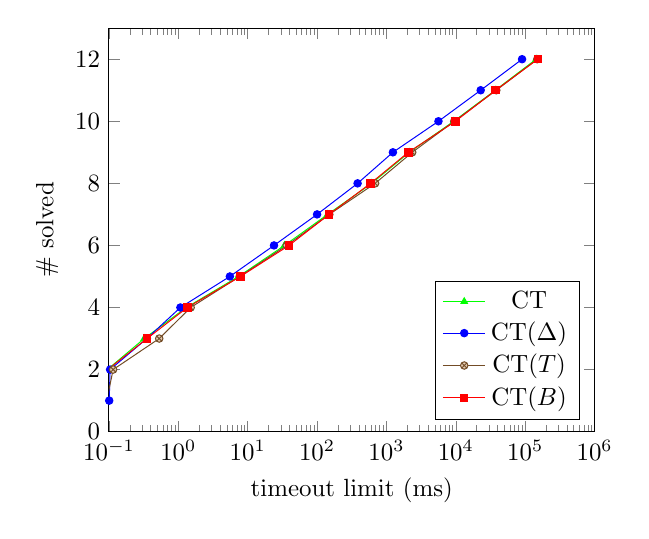
\begin{tikzpicture}[scale=0.9]
        \begin{axis}[
    xmode=log,
    ymin=0,ymax=13,
    xmin=0.1, xmax=1000000,
    every axis plot/.style={thin},
    xlabel={timeout limit (ms)},
    ylabel={\# solved},
    legend pos=south east
    % table/create on use/cumulative distribution/.style={
    %   create col/expr={\pgfmathaccuma + \thisrow{f(x)}}   
    % }
    ]
    \addplot 
    [mark=triangle*,
    mark size=1.5,
    mark options={solid},
    green] 
    coordinates {(0.092, 1)
(0.095, 2)
(0.323, 3)
(1.305, 4)
(7.407, 5)
(33.999, 6)
(142.189, 7)
(612.106, 8)
(2128.536, 9)
(9342.811, 10)
(37031.905, 11)
(143593.524, 12)};

    \addplot 
    [blue,
    mark=*,
    mark size=1.5,
    mark options={solid}]
    coordinates {(0.101, 1)
(0.104, 2)
(0.352, 3)
(1.072, 4)
(5.534, 5)
(23.943, 6)
(100.074, 7)
(383.914, 8)
(1238.844, 9)
(5618.200, 10)
(22809.152, 11)
(90056.907, 12)};

    \addplot [brown!60!black,
    mark options={fill=brown!40},
    mark=otimes*,
    mark size=1.5]
    coordinates {(0.093, 1)
(0.115, 2)
(0.531, 3)
(1.508, 4)
(7.667, 5)
(36.564, 6)
(150.260, 7)
(687.096, 8)
(2352.488, 9)
(9484.143, 10)
(38304.007, 11)
(149005.215, 12)};

    \addplot 
    [red,
    mark size=1.5,
    mark=square*]
    coordinates {(0.095, 1)
(0.096, 2)
(0.355, 3)
(1.348, 4)
(7.869, 5)
(39.453, 6)
(149.173, 7)
(590.206, 8)
(2064.396, 9)
(9858.869, 10)
(37441.670, 11)
(151868.885, 12)};
    \legend{CT,CT($\Delta$),CT($T$),CT($B$)}
  \end{axis}

    \end{tikzpicture}
    \vfill
    \caption{\textbf{Langford 4}.}
    \vspace{\baselineskip}
  \end{minipage}\qquad
  \begin{minipage}[b][8cm][s]{0.45\textwidth}
    \centering
    \vfill
    \begin{tikzpicture}[scale=0.9]
      \begin{tikzpicture}[scale=1.0]
  \begin{axis}[
    xmode=log,
    ymin=0,ymax=50,
    xmin=0.1, xmax=1000000,
    every axis plot/.style={thin},
    xlabel={timeout limit (ms)},
    ylabel={\# solved},
    legend pos=south east
    % table/create on use/cumulative distribution/.style={
    %   create col/expr={\pgfmathaccuma + \thisrow{f(x)}}   
    % }
    ]
    \addplot 
    [mark=triangle*,
    mark size=1.5,
    mark options={solid},
    green] 
    coordinates {(4616.454, 1)
(4618.833, 2)
(4940.533, 3)
(4966.402, 4)
(5022.930, 5)
(5116.613, 6)
(5130.681, 7)
(5134.031, 8)
(5193.654, 9)
(5285.091, 10)
(5305.009, 11)
(5328.617, 12)
(5371.012, 13)
(5388.793, 14)
(5410.720, 15)
(5441.997, 16)
(5455.481, 17)
(5578.855, 18)
(5641.853, 19)
(5648.097, 20)
(5672.192, 21)
(5679.702, 22)
(5683.292, 23)
(5719.242, 24)
(5725.902, 25)
(5734.356, 26)
(5760.307, 27)
(5771.703, 28)
(5797.243, 29)
(5849.862, 30)
(5898.012, 31)
(5937.207, 32)
(6002.529, 33)
(6019.686, 34)
(6119.094, 35)
(6158.836, 36)
(6199.964, 37)
(6257.022, 38)
(6279.015, 39)
(6296.990, 40)
(6352.257, 41)
(6430.852, 42)
(6432.519, 43)
(6470.687, 44)
(6490.446, 45)
(6539.759, 46)
(6552.644, 47)
(6577.534, 48)
(6645.354, 49)
(6760.127, 50)};

    \addplot 
    [blue,
    mark=*,
    mark size=1.5,
    mark options={solid}]
    coordinates {(2221.627, 1)
(2406.818, 2)
(2410.417, 3)
(2478.595, 4)
(2494.484, 5)
(2610.324, 6)
(2662.381, 7)
(2699.699, 8)
(2701.623, 9)
(2705.606, 10)
(2723.756, 11)
(2737.326, 12)
(2765.084, 13)
(2766.971, 14)
(2799.027, 15)
(2809.753, 16)
(2858.020, 17)
(2883.670, 18)
(2887.618, 19)
(2899.053, 20)
(2909.206, 21)
(2912.107, 22)
(2971.321, 23)
(2982.026, 24)
(3005.557, 25)
(3013.018, 26)
(3025.735, 27)
(3030.892, 28)
(3114.959, 29)
(3119.511, 30)
(3123.651, 31)
(3124.390, 32)
(3148.031, 33)
(3176.451, 34)
(3193.730, 35)
(3266.242, 36)
(3304.264, 37)
(3313.805, 38)
(3330.655, 39)
(3362.242, 40)
(3371.608, 41)
(3501.498, 42)
(3523.099, 43)
(3530.659, 44)
(3556.029, 45)
(3582.482, 46)
(3592.317, 47)
(3604.448, 48)
(3685.513, 49)
(3744.809, 50)};

    \addplot [brown!60!black,
    mark options={fill=brown!40},
    mark=otimes*,
    mark size=1.5]
    coordinates {(4666.117, 1)
(4884.063, 2)
(5090.625, 3)
(5188.099, 4)
(5305.729, 5)
(5361.245, 6)
(5455.278, 7)
(5457.351, 8)
(5473.296, 9)
(5522.072, 10)
(5560.972, 11)
(5598.913, 12)
(5605.940, 13)
(5609.929, 14)
(5654.246, 15)
(5661.025, 16)
(5716.926, 17)
(5727.477, 18)
(5742.211, 19)
(5789.404, 20)
(5869.049, 21)
(5875.201, 22)
(5891.779, 23)
(5911.066, 24)
(5919.859, 25)
(5927.269, 26)
(6068.873, 27)
(6113.292, 28)
(6171.700, 29)
(6197.012, 30)
(6241.185, 31)
(6308.864, 32)
(6314.385, 33)
(6328.125, 34)
(6361.133, 35)
(6450.681, 36)
(6454.027, 37)
(6480.689, 38)
(6493.962, 39)
(6503.325, 40)
(6578.864, 41)
(6597.842, 42)
(6626.283, 43)
(6635.984, 44)
(6662.996, 45)
(6684.042, 46)
(6880.051, 47)
(6924.437, 48)
(7090.997, 49)
(7478.901, 50)};

    \addplot 
    [red,
    mark size=1.5,
    mark=square*]
    coordinates {(5703.521, 1)
(5738.525, 2)
(6124.676, 3)
(6219.223, 4)
(6269.173, 5)
(6319.573, 6)
(6395.842, 7)
(6475.436, 8)
(6503.743, 9)
(6517.282, 10)
(6560.928, 11)
(6588.592, 12)
(6615.815, 13)
(6658.460, 14)
(6693.669, 15)
(6714.939, 16)
(6725.284, 17)
(6734.258, 18)
(6737.600, 19)
(6786.792, 20)
(6882.622, 21)
(6944.081, 22)
(6954.326, 23)
(7000.798, 24)
(7002.849, 25)
(7194.996, 26)
(7286.496, 27)
(7364.088, 28)
(7411.608, 29)
(7610.262, 30)
(7610.536, 31)
(7618.013, 32)
(7647.617, 33)
(7713.546, 34)
(7745.128, 35)
(7781.769, 36)
(7838.707, 37)
(7911.546, 38)
(7945.896, 39)
(7963.194, 40)
(8066.271, 41)
(8067.345, 42)
(8099.522, 43)
(8122.602, 44)
(8123.710, 45)
(8140.318, 46)
(8293.420, 47)
(8360.070, 48)
(8378.116, 49)
(8579.463, 50)};
    \legend{CT,D,F,L}
  \end{axis}
\end{tikzpicture}

    \end{tikzpicture}
    \vfill
    \caption{\textbf{A5}.}
    \vspace{\baselineskip}
  \end{minipage}\qquad

\end{figure}

\begin{figure}
  \begin{minipage}[b][8cm][s]{0.45\textwidth}
    \centering
    \vfill
    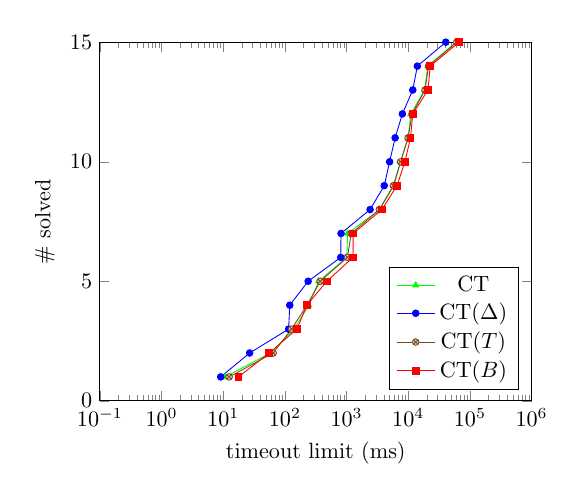
\begin{tikzpicture}[scale=0.8]
        \begin{axis}[
    xmode=log,
    ymin=0,ymax=15,
    xmin=0.1, xmax=1000000,
    every axis plot/.style={thin},
    xlabel={timeout limit (ms)},
    ylabel={\# solved},
    legend pos=south east
    % table/create on use/cumulative distribution/.style={
    %   create col/expr={\pgfmathaccuma + \thisrow{f(x)}}   
    % }
    ]
    \addplot 
    [mark=triangle*,
    mark size=1.5,
    mark options={solid},
    green] 
    coordinates {(10.724, 1)
(58.141, 2)
(140.926, 3)
(244.339, 4)
(351.655, 5)
(1007.846, 6)
(1040.618, 7)
(3429.804, 8)
(5862.337, 9)
(7518.829, 10)
(9922.216, 11)
(10995.644, 12)
(18421.925, 13)
(20703.909, 14)
(59350.857, 15)};

    \addplot 
    [blue,
    mark=*,
    mark size=1.5,
    mark options={solid}]
    coordinates {(9.092, 1)
(26.766, 2)
(114.809, 3)
(119.817, 4)
(237.752, 5)
(803.879, 6)
(812.209, 7)
(2403.255, 8)
(4081.014, 9)
(4986.668, 10)
(6124.842, 11)
(8030.718, 12)
(11828.045, 13)
(14031.517, 14)
(40586.867, 15)};

    \addplot [brown!60!black,
    mark options={fill=brown!40},
    mark=otimes*,
    mark size=1.5]
    coordinates {(12.465, 1)
(64.573, 2)
(127.898, 3)
(228.109, 4)
(372.722, 5)
(1029.302, 6)
(1191.482, 7)
(3392.266, 8)
(5728.998, 9)
(7496.585, 10)
(9916.094, 11)
(11510.717, 12)
(18700.846, 13)
(21320.804, 14)
(60889.133, 15)};

    \addplot 
    [red,
    mark size=1.5,
    mark=square*]
    coordinates {(17.667, 1)
(55.690, 2)
(156.556, 3)
(226.984, 4)
(477.676, 5)
(1271.053, 6)
(1280.040, 7)
(3730.514, 8)
(6571.512, 9)
(8823.766, 10)
(10881.983, 11)
(11821.394, 12)
(20882.392, 13)
(22667.922, 14)
(66608.065, 15)};
\legend{CT,CT($\Delta$),CT($T$),CT($B$)}
  \end{axis}

    \end{tikzpicture}
    \vfill
    \caption{\textbf{TSP Quat 20}.}
    \vspace{\baselineskip}
  \end{minipage}\qquad
  \begin{minipage}[b][8cm][s]{0.45\textwidth}
    \centering
    \vfill
    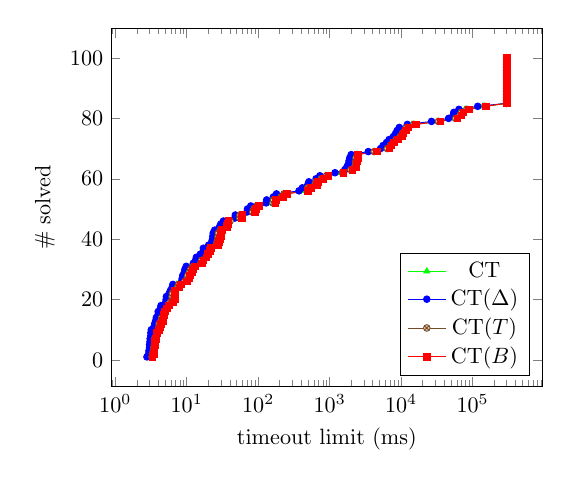
\begin{tikzpicture}[scale=0.8]
        \begin{axis}[
    xmode=log,
    every axis plot/.style={thin},
    xlabel={timeout limit (ms)},
    ylabel={\# solved},
    legend pos=south east
    % table/create on use/cumulative distribution/.style={
    %   create col/expr={\pgfmathaccuma + \thisrow{f(x)}}   
    % }
    ]
    \addplot 
    [mark=triangle*,
    mark size=1.5,
    mark options={solid},
    green] 
    coordinates {(3.196, 1)
(3.216, 2)
(3.219, 3)
(3.229, 4)
(3.236, 5)
(3.323, 6)
(3.324, 7)
(3.384, 8)
(3.555, 9)
(3.581, 10)
(3.920, 11)
(4.054, 12)
(4.316, 13)
(4.359, 14)
(4.438, 15)
(4.766, 16)
(4.899, 17)
(5.467, 18)
(5.778, 19)
(5.909, 20)
(5.980, 21)
(6.063, 22)
(6.737, 23)
(6.982, 24)
(7.263, 25)
(9.535, 26)
(9.722, 27)
(9.747, 28)
(10.539, 29)
(10.888, 30)
(11.322, 31)
(14.686, 32)
(15.476, 33)
(16.077, 34)
(17.910, 35)
(19.693, 36)
(19.701, 37)
(25.391, 38)
(25.547, 39)
(26.324, 40)
(27.363, 41)
(27.371, 42)
(28.865, 43)
(33.178, 44)
(33.245, 45)
(37.119, 46)
(53.644, 47)
(55.989, 48)
(79.967, 49)
(80.956, 50)
(91.520, 51)
(153.402, 52)
(158.352, 53)
(208.937, 54)
(228.227, 55)
(459.054, 56)
(495.212, 57)
(617.786, 58)
(634.692, 59)
(768.712, 60)
(875.114, 61)
(1437.146, 62)
(1905.669, 63)
(2114.601, 64)
(2212.913, 65)
(2220.314, 66)
(2259.432, 67)
(2410.211, 68)
(4177.779, 69)
(6168.465, 70)
(6834.469, 71)
(7334.068, 72)
(8282.489, 73)
(9512.268, 74)
(9927.672, 75)
(10947.310, 76)
(11558.129, 77)
(14232.711, 78)
(32770.476, 79)
(54494.164, 80)
(63805.832, 81)
(66673.105, 82)
(78558.979, 83)
(139323.248, 84)
(300000.148, 85)
(300000.170, 86)
(300000.230, 87)
(300000.269, 88)
(300000.313, 89)
(300000.395, 90)
(300000.426, 91)
(300000.491, 92)
(300000.615, 93)
(300000.626, 94)
(300000.663, 95)
(300000.758, 96)
(300000.834, 97)
(300000.901, 98)
(300001.161, 99)
(300001.278, 100)};

    \addplot 
    [blue,
    mark=*,
    mark size=1.5,
    mark options={solid}]
    coordinates {(2.777, 1)
(2.935, 2)
(2.962, 3)
(3.017, 4)
(3.019, 5)
(3.065, 6)
(3.077, 7)
(3.142, 8)
(3.150, 9)
(3.195, 10)
(3.490, 11)
(3.569, 12)
(3.687, 13)
(3.755, 14)
(3.975, 15)
(3.989, 16)
(4.273, 17)
(4.370, 18)
(5.066, 19)
(5.146, 20)
(5.199, 21)
(5.672, 22)
(5.925, 23)
(6.237, 24)
(6.405, 25)
(8.452, 26)
(8.651, 27)
(8.811, 28)
(9.254, 29)
(9.443, 30)
(9.845, 31)
(12.377, 32)
(13.285, 33)
(13.648, 34)
(15.465, 35)
(16.998, 36)
(17.089, 37)
(20.222, 38)
(22.259, 39)
(22.952, 40)
(23.206, 41)
(23.466, 42)
(24.612, 43)
(28.672, 44)
(29.937, 45)
(32.603, 46)
(47.179, 47)
(47.867, 48)
(69.677, 49)
(70.818, 50)
(78.794, 51)
(128.883, 52)
(131.422, 53)
(163.522, 54)
(180.337, 55)
(372.882, 56)
(414.876, 57)
(494.062, 58)
(511.910, 59)
(646.291, 60)
(729.479, 61)
(1187.909, 62)
(1627.029, 63)
(1746.098, 64)
(1833.159, 65)
(1870.757, 66)
(1917.989, 67)
(2005.271, 68)
(3468.723, 69)
(5153.090, 70)
(5590.949, 71)
(6253.125, 72)
(6807.754, 73)
(7789.728, 74)
(8368.926, 75)
(8804.268, 76)
(9432.540, 77)
(12223.062, 78)
(26637.130, 79)
(46105.675, 80)
(53283.710, 81)
(54647.876, 82)
(64363.777, 83)
(117915.726, 84)
(298513.851, 85)
(300000.155, 86)
(300000.231, 87)
(300000.251, 88)
(300000.327, 89)
(300000.341, 90)
(300000.397, 91)
(300000.468, 92)
(300000.469, 93)
(300000.508, 94)
(300000.556, 95)
(300000.575, 96)
(300000.651, 97)
(300000.702, 98)
(300000.711, 99)
(300000.912, 100)};

    \addplot [brown!60!black,
    mark options={fill=brown!40},
    mark=otimes*,
    mark size=1.5]
    coordinates {(3.271, 1)
(3.312, 2)
(3.413, 3)
(3.445, 4)
(3.513, 5)
(3.542, 6)
(3.545, 7)
(3.729, 8)
(3.847, 9)
(3.970, 10)
(4.064, 11)
(4.123, 12)
(4.357, 13)
(4.451, 14)
(4.827, 15)
(4.949, 16)
(5.189, 17)
(5.741, 18)
(5.832, 19)
(6.224, 20)
(6.239, 21)
(6.291, 22)
(6.663, 23)
(7.391, 24)
(7.727, 25)
(9.374, 26)
(10.126, 27)
(10.353, 28)
(10.850, 29)
(11.372, 30)
(12.360, 31)
(15.600, 32)
(16.099, 33)
(18.668, 34)
(20.124, 35)
(20.584, 36)
(22.324, 37)
(25.523, 38)
(26.453, 39)
(27.049, 40)
(27.494, 41)
(27.631, 42)
(29.306, 43)
(35.334, 44)
(36.200, 45)
(40.453, 46)
(55.257, 47)
(55.730, 48)
(83.536, 49)
(86.982, 50)
(96.644, 51)
(160.664, 52)
(163.689, 53)
(208.757, 54)
(229.167, 55)
(491.046, 56)
(491.402, 57)
(620.464, 58)
(644.970, 59)
(759.047, 60)
(903.670, 61)
(1512.925, 62)
(1978.608, 63)
(2256.797, 64)
(2300.228, 65)
(2328.132, 66)
(2339.827, 67)
(2441.904, 68)
(4189.045, 69)
(6398.233, 70)
(7059.747, 71)
(7672.819, 72)
(8532.069, 73)
(9683.204, 74)
(10419.366, 75)
(11199.375, 76)
(12061.647, 77)
(15029.916, 78)
(33283.823, 79)
(57881.236, 80)
(66474.073, 81)
(69399.642, 82)
(83281.381, 83)
(148458.146, 84)
(300000.162, 85)
(300000.163, 86)
(300000.270, 87)
(300000.280, 88)
(300000.298, 89)
(300000.307, 90)
(300000.316, 91)
(300000.345, 92)
(300000.405, 93)
(300000.419, 94)
(300000.420, 95)
(300000.442, 96)
(300000.548, 97)
(300000.623, 98)
(300000.805, 99)
(300001.376, 100)};

    \addplot 
    [red,
    mark size=1.5,
    mark=square*]
    coordinates {(3.316, 1)
(3.470, 2)
(3.518, 3)
(3.551, 4)
(3.592, 5)
(3.600, 6)
(3.735, 7)
(3.762, 8)
(3.816, 9)
(4.053, 10)
(4.313, 11)
(4.324, 12)
(4.630, 13)
(4.718, 14)
(4.822, 15)
(4.913, 16)
(5.339, 17)
(5.672, 18)
(6.475, 19)
(6.796, 20)
(6.800, 21)
(6.859, 22)
(6.869, 23)
(7.940, 24)
(8.327, 25)
(10.053, 26)
(10.887, 27)
(11.163, 28)
(11.941, 29)
(12.236, 30)
(13.002, 31)
(16.476, 32)
(17.063, 33)
(18.833, 34)
(19.634, 35)
(21.271, 36)
(21.980, 37)
(27.160, 38)
(28.307, 39)
(29.288, 40)
(29.853, 41)
(30.301, 42)
(31.279, 43)
(36.647, 44)
(37.576, 45)
(38.220, 46)
(59.212, 47)
(60.439, 48)
(90.691, 49)
(93.609, 50)
(102.648, 51)
(175.123, 52)
(175.969, 53)
(226.712, 54)
(251.960, 55)
(500.551, 56)
(550.919, 57)
(669.924, 58)
(681.833, 59)
(817.046, 60)
(960.972, 61)
(1559.428, 62)
(2083.045, 63)
(2366.282, 64)
(2378.071, 65)
(2435.825, 66)
(2502.688, 67)
(2505.391, 68)
(4558.792, 69)
(6832.511, 70)
(7291.945, 71)
(8012.142, 72)
(9077.137, 73)
(10207.670, 74)
(10790.878, 75)
(11695.497, 76)
(12715.296, 77)
(15991.589, 78)
(35343.944, 79)
(61685.336, 80)
(69906.557, 81)
(74635.852, 82)
(88544.807, 83)
(152679.605, 84)
(300000.253, 85)
(300000.287, 86)
(300000.324, 87)
(300000.329, 88)
(300000.332, 89)
(300000.344, 90)
(300000.345, 91)
(300000.390, 92)
(300000.398, 93)
(300000.511, 94)
(300000.522, 95)
(300000.523, 96)
(300000.694, 97)
(300000.757, 98)
(300000.769, 99)
(300001.051, 100)};
    \legend{CT,CT($\Delta$),CT($T$),CT($B$)}
  \end{axis}

    \end{tikzpicture}
    \vfill
    \caption{\textbf{Geom}.}
    \vspace{\baselineskip}
  \end{minipage}\qquad
  \begin{minipage}[b][8cm][s]{0.45\textwidth}
    \centering
    \vfill
    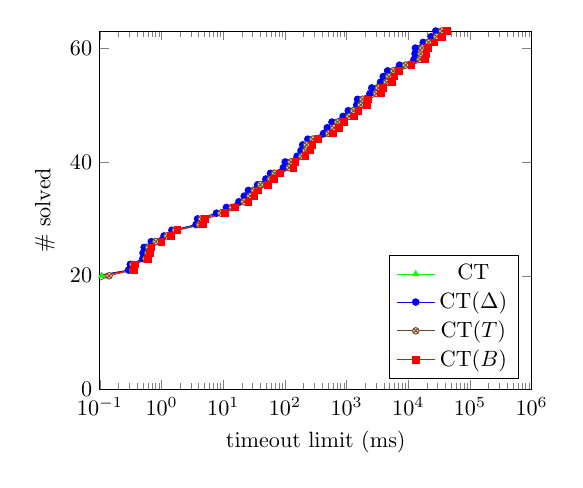
\begin{tikzpicture}[scale=0.8]
        \begin{axis}[
    xmode=log,
    ymin=0,ymax=63,
    xmin=0.1, xmax=1000000,
    every axis plot/.style={thin},
    xlabel={timeout limit (ms)},
    ylabel={\# solved},
    legend pos=south east
    % table/create on use/cumulative distribution/.style={
    %   create col/expr={\pgfmathaccuma + \thisrow{f(x)}}   
    % }
    ]
    \addplot 
    [mark=triangle*,
    mark size=1.5,
    mark options={solid},
    green] 
    coordinates {(0.061, 1)
(0.063, 2)
(0.063, 3)
(0.063, 4)
(0.066, 5)
(0.066, 6)
(0.067, 7)
(0.067, 8)
(0.068, 9)
(0.068, 10)
(0.068, 11)
(0.069, 12)
(0.069, 13)
(0.070, 14)
(0.072, 15)
(0.077, 16)
(0.077, 17)
(0.078, 18)
(0.087, 19)
(0.107, 20)
(0.302, 21)
(0.319, 22)
(0.546, 23)
(0.558, 24)
(0.571, 25)
(0.769, 26)
(1.228, 27)
(1.712, 28)
(4.017, 29)
(4.420, 30)
(8.986, 31)
(13.140, 32)
(22.686, 33)
(25.984, 34)
(29.793, 35)
(41.355, 36)
(57.374, 37)
(68.504, 38)
(120.233, 39)
(125.250, 40)
(187.928, 41)
(215.122, 42)
(239.080, 43)
(279.547, 44)
(521.134, 45)
(614.516, 46)
(709.564, 47)
(1052.148, 48)
(1307.717, 49)
(1711.958, 50)
(1808.349, 51)
(2960.202, 52)
(3082.804, 53)
(4377.795, 54)
(4793.723, 55)
(5700.589, 56)
(9022.380, 57)
(15776.713, 58)
(15978.109, 59)
(17078.488, 60)
(21737.971, 61)
(28889.226, 62)
(35570.896, 63)};

    \addplot 
    [blue,
    mark=*,
    mark size=1.5,
    mark options={solid}]
    coordinates {(0.063, 1)
(0.063, 2)
(0.064, 3)
(0.064, 4)
(0.065, 5)
(0.066, 6)
(0.066, 7)
(0.067, 8)
(0.067, 9)
(0.068, 10)
(0.070, 11)
(0.071, 12)
(0.072, 13)
(0.073, 14)
(0.077, 15)
(0.081, 16)
(0.084, 17)
(0.084, 18)
(0.084, 19)
(0.086, 20)
(0.291, 21)
(0.311, 22)
(0.496, 23)
(0.501, 24)
(0.521, 25)
(0.681, 26)
(1.096, 27)
(1.469, 28)
(3.628, 29)
(3.832, 30)
(7.775, 31)
(11.243, 32)
(17.914, 33)
(21.871, 34)
(25.542, 35)
(36.155, 36)
(48.984, 37)
(58.236, 38)
(94.364, 39)
(100.877, 40)
(157.529, 41)
(182.301, 42)
(194.176, 43)
(235.119, 44)
(423.000, 45)
(485.117, 46)
(579.516, 47)
(876.517, 48)
(1064.927, 49)
(1457.682, 50)
(1503.779, 51)
(2387.354, 52)
(2560.341, 53)
(3544.655, 54)
(3925.391, 55)
(4620.278, 56)
(7208.727, 57)
(12396.750, 58)
(12860.648, 59)
(13052.702, 60)
(17468.947, 61)
(23419.166, 62)
(27937.226, 63)};

    \addplot [brown!60!black,
    mark options={fill=brown!40},
    mark=otimes*,
    mark size=1.5]
    coordinates {(0.064, 1)
(0.064, 2)
(0.065, 3)
(0.066, 4)
(0.067, 5)
(0.067, 6)
(0.068, 7)
(0.069, 8)
(0.070, 9)
(0.071, 10)
(0.072, 11)
(0.072, 12)
(0.072, 13)
(0.072, 14)
(0.074, 15)
(0.080, 16)
(0.090, 17)
(0.090, 18)
(0.091, 19)
(0.141, 20)
(0.336, 21)
(0.342, 22)
(0.558, 23)
(0.601, 24)
(0.617, 25)
(0.809, 26)
(1.230, 27)
(1.673, 28)
(4.117, 29)
(4.428, 30)
(9.151, 31)
(13.889, 32)
(21.704, 33)
(27.173, 34)
(31.645, 35)
(40.064, 36)
(58.053, 37)
(68.236, 38)
(117.377, 39)
(125.492, 40)
(187.061, 41)
(216.572, 42)
(225.602, 43)
(282.555, 44)
(509.215, 45)
(621.611, 46)
(714.553, 47)
(1099.519, 48)
(1292.777, 49)
(1695.555, 50)
(1819.323, 51)
(3040.647, 52)
(3268.028, 53)
(4477.302, 54)
(4845.251, 55)
(5745.500, 56)
(9046.983, 57)
(15446.323, 58)
(15974.990, 59)
(16826.034, 60)
(21335.821, 61)
(28793.599, 62)
(35220.653, 63)};

    \addplot 
    [red,
    mark size=1.5,
    mark=square*]
    coordinates {(0.061, 1)
(0.062, 2)
(0.064, 3)
(0.065, 4)
(0.065, 5)
(0.066, 6)
(0.066, 7)
(0.066, 8)
(0.070, 9)
(0.070, 10)
(0.070, 11)
(0.073, 12)
(0.074, 13)
(0.074, 14)
(0.075, 15)
(0.076, 16)
(0.078, 17)
(0.078, 18)
(0.078, 19)
(0.096, 20)
(0.355, 21)
(0.368, 22)
(0.602, 23)
(0.649, 24)
(0.687, 25)
(0.990, 26)
(1.429, 27)
(1.803, 28)
(4.679, 29)
(5.060, 30)
(10.702, 31)
(15.639, 32)
(25.674, 33)
(32.030, 34)
(36.240, 35)
(53.128, 36)
(66.758, 37)
(83.306, 38)
(137.119, 39)
(147.946, 40)
(215.703, 41)
(259.463, 42)
(280.813, 43)
(344.304, 44)
(601.474, 45)
(750.007, 46)
(896.055, 47)
(1302.781, 48)
(1548.165, 49)
(2114.331, 50)
(2229.336, 51)
(3648.636, 52)
(3875.425, 53)
(5405.249, 54)
(5972.155, 55)
(7115.776, 56)
(11299.423, 57)
(18763.604, 58)
(19787.189, 59)
(20634.353, 60)
(26647.401, 61)
(35053.136, 62)
(42731.494, 63)};
    \legend{CT,CT($\Delta$),CT($T$),CT($B$)}
  \end{axis}

    \end{tikzpicture}
    \vfill
    \caption{\textbf{Crosswords LexVG}.}
    \vspace{\baselineskip}
  \end{minipage} \qquad
    \begin{minipage}[b][8cm][s]{0.45\textwidth}
    \centering
    \vfill
    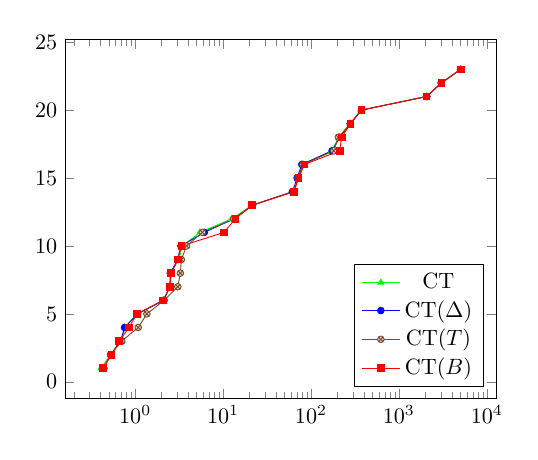
\begin{tikzpicture}[scale=0.8]
      \begin{axis}[
    xmode=log,
    every axis plot/.style={thin},
    legend pos=south east
    % table/create on use/cumulative distribution/.style={
    %   create col/expr={\pgfmathaccuma + \thisrow{f(x)}}   
    % }
    ]
    \addplot 
    [mark=triangle*,
    mark size=1.5,
    mark options={solid},
    green] 
    coordinates {
    (0.408, 1)
(0.522, 2)
(0.709, 3)
(0.760, 4)
(1.056, 5)
(2.080, 6)
(2.498, 7)
(2.545, 8)
(3.130, 9)
(3.455, 10)
(5.443, 11)
(12.540, 12)
(21.400, 13)
(63.357, 14)
(72.327, 15)
(78.959, 16)
(171.759, 17)
(206.671, 18)
(277.940, 19)
(368.226, 20)
(2055.906, 21)
(3069.686, 22)
(5042.018, 23)
    };

    \addplot 
    [blue,
    mark=*,
    mark size=1.5,
    mark options={solid}]
    coordinates {
    (0.435, 1)
(0.527, 2)
(0.682, 3)
(0.757, 4)
(1.064, 5)
(2.119, 6)
(2.471, 7)
(2.506, 8)
(3.033, 9)
(3.313, 10)
(6.107, 11)
(13.333, 12)
(21.562, 13)
(61.519, 14)
(69.514, 15)
(78.605, 16)
(173.735, 17)
(212.749, 18)
(279.236, 19)
(376.528, 20)
(2079.356, 21)
(3025.003, 22)
(5055.306, 23)
    };

    \addplot [brown!60!black,
    mark options={fill=brown!40},
    mark=otimes*,
    mark size=1.5]
    coordinates {
    (0.441, 1)
(0.524, 2)
(0.703, 3)
(1.082, 4)
(1.358, 5)
(2.130, 6)
(3.051, 7)
(3.265, 8)
(3.349, 9)
(3.843, 10)
(5.818, 11)
(13.296, 12)
(21.610, 13)
(63.892, 14)
(71.335, 15)
(81.227, 16)
(181.520, 17)
(204.798, 18)
(281.310, 19)
(374.836, 20)
(2064.777, 21)
(3039.022, 22)
(5009.530, 23)
    };

    \addplot 
    [red,
    mark size=1.5,
    mark=square*]
    coordinates {
    (0.428, 1)
(0.539, 2)
(0.658, 3)
(0.848, 4)
(1.050, 5)
(2.068, 6)
(2.501, 7)
(2.568, 8)
(3.061, 9)
(3.359, 10)
(10.237, 11)
(13.760, 12)
(21.391, 13)
(64.274, 14)
(72.091, 15)
(84.141, 16)
(211.811, 17)
(223.544, 18)
(281.354, 19)
(373.329, 20)
(2057.236, 21)
(3040.006, 22)
(5040.147, 23)
    };
    \legend{CT,CT($\Delta$),CT($T$),CT($B$)}
  \end{axis}

    \end{tikzpicture}
    \vfill
    \caption{\textbf{AIM 50}.}
    \vspace{\baselineskip}
  \end{minipage} \qquad
  
\end{figure}

\clearpage

\section{Plots from Comparison of CT against Existing Propagators}
\label{app:compare-gecode}

Each plot shows the number of instances solved as a function
of timeout limit in milliseconds. The leftmost column shows 
runtime,
the rightmost column shows solve time.

\Todo{Todo: One figure per serie, referring to left/right does not work.}


\newpage

\begin{figure}
  \begin{minipage}[b][10cm][s]{0.45\textwidth}
    \centering
    \vfill
    \begin{tikzpicture}[scale=0.8]
      \begin{axis}[
    xmode=log,
    ymin=0,ymax=20,
    xmin=0.1, xmax=1000000,
    every axis plot/.style={thin},
    xlabel={timeout limit (ms)},
    ylabel={\# solved},
    legend pos=south east
    % table/create on use/cumulative distribution/.style={
    %   create col/expr={\pgfmathaccuma + \thisrow{f(x)}}   
    % }
    ]
    \addplot 
    [mark=triangle*,
    mark size=1.5,
    mark options={solid},
    green] 
    coordinates {(0.088, 1)
(0.182, 2)
(0.233, 3)
(0.942, 4)
(1.622, 5)
(4.020, 6)
(7.439, 7)
(7.733, 8)
(8.229, 9)
(10.629, 10)
(16.624, 11)
(40.292, 12)
(67.440, 13)
(1244.797, 14)
(7858.266, 15)
(1000001.583, 16)
(1000001.852, 17)
(1009212.178, 18)
(1012657.780, 19)
(1012814.040, 20)};

    \addplot 
    [blue,
    mark=*,
    mark size=1.5,
    mark options={solid}]
    coordinates {(0.084, 1)
(0.206, 2)
(0.217, 3)
(0.871, 4)
(1.393, 5)
(4.322, 6)
(7.026, 7)
(7.901, 8)
(7.904, 9)
(10.663, 10)
(18.990, 11)
(50.266, 12)
(96.214, 13)
(1467.636, 14)
(9916.340, 15)
(1000001.971, 16)
(1000002.938, 17)
(1000004.363, 18)
(1000005.402, 19)
(1000011.197, 20)};

    \addplot [brown!60!black,
    mark options={fill=brown!40},
    mark=otimes*,
    mark size=1.5]
    table {(0.087, 1)
(0.236, 2)
(0.311, 3)
(1.152, 4)
(1.786, 5)
(5.762, 6)
(8.968, 7)
(10.301, 8)
(10.566, 9)
(15.086, 10)
(23.403, 11)
(63.558, 12)
(119.651, 13)
(1877.973, 14)
(13098.088, 15)
(1000002.296, 16)
(1000003.170, 17)
(1000007.159, 18)
(1000007.877, 19)
(1000015.365, 20)};

    \addplot 
    [red,
    mark size=1.5,
    mark=square*]
    table {(0.081, 1)
(0.157, 2)
(0.223, 3)
(0.596, 4)
(0.895, 5)
(2.233, 6)
(4.192, 7)
(4.233, 8)
(4.349, 9)
(5.717, 10)
(8.703, 11)
(21.423, 12)
(37.126, 13)
(669.099, 14)
(4203.782, 15)
(1000000.429, 16)
(1000000.554, 17)
(1000000.652, 18)
(1000000.873, 19)
(1000001.178, 20)};
    \legend{Reg,Tup\_mem,Tup\_speed,CT}
  \end{axis}

    \end{tikzpicture}
    \vfill
    \caption{\textbf{Langford 2}. The 20 instances
    of this benchmark contain binary constraints.
    The variable domains vary from 0..5 to 0..41.}
    \vspace{\baselineskip}
  \end{minipage}\qquad
  \begin{minipage}[b][10cm][s]{0.45\textwidth}
    \centering
    \vfill
    \begin{tikzpicture}[scale=0.8]
      \begin{axis}[
    xmode=log,
    ymin=0,ymax=16,
    xmin=0.1, xmax=1000000,
    every axis plot/.style={thin},
    xlabel={timeout limit (ms)},
    ylabel={\# solved},
    legend pos=south east
    % table/create on use/cumulative distribution/.style={
    %   create col/expr={\pgfmathaccuma + \thisrow{f(x)}}   
    % }
    ]
    \addplot 
    [mark=triangle*,
    mark size=1.5,
    mark options={solid},
    green] 
    coordinates {(0.101, 1)
(0.159, 2)
(0.385, 3)
(1.631, 4)
(6.760, 5)
(27.796, 6)
(130.974, 7)
(131.594, 8)
(460.229, 9)
(11472.663, 10)
(18145.843, 11)
(53170.447, 12)
(281456.879, 13)
(1000007.563, 14)
(1000007.588, 15)
(1000013.342, 16)};

    \addplot 
    [blue,
    mark=*,
    mark size=1.5,
    mark options={solid}]
    coordinates {(0.076, 1)
(0.129, 2)
(0.375, 3)
(1.684, 4)
(6.892, 5)
(35.105, 6)
(146.741, 7)
(167.561, 8)
(642.014, 9)
(18202.298, 10)
(42684.881, 11)
(82959.726, 12)
(490547.070, 13)
(1000011.196, 14)
(1000016.557, 15)
(1000016.694, 16)};

    \addplot [brown!60!black,
    mark options={fill=brown!40},
    mark=otimes*,
    mark size=1.5]
    table {(0.090, 1)
(0.166, 2)
(0.510, 3)
(2.198, 4)
(8.900, 5)
(37.617, 6)
(192.203, 7)
(218.167, 8)
(737.821, 9)
(20345.581, 10)
(46306.577, 11)
(103637.500, 12)
(597597.517, 13)
(1000020.102, 14)
(1000020.695, 15)
(1000030.283, 16)};

    \addplot 
    [red,
    mark size=1.5,
    mark=square*]
    table {(0.084, 1)
(0.120, 2)
(0.282, 3)
(1.077, 4)
(4.754, 5)
(20.901, 6)
(95.743, 7)
(100.046, 8)
(388.791, 9)
(9911.345, 10)
(20137.299, 11)
(50724.854, 12)
(291121.550, 13)
(1000003.563, 14)
(1000003.963, 15)
(1000006.252, 16)};
    \legend{Reg,Tup\_mem,Tup\_speed,CT}
  \end{axis}

    \end{tikzpicture}
    \vfill
    \caption{\textbf{Langford 3}. The 16 instances
    of this benchmark contain binary constraints.
    The variable domains vary from 0..5 to 0..50.}
    \vspace{\baselineskip}
  \end{minipage}\qquad
  \begin{minipage}[b][10cm][s]{0.45\textwidth}
    \centering
    \vfill
    \begin{tikzpicture}[scale=0.8]
      \begin{axis}[
    xmode=log,
    ymin=0,ymax=12,
    xmin=0.1, xmax=1000000,
    every axis plot/.style={thin},
    xlabel={timeout limit (ms)},
    ylabel={\# solved},
    legend pos=south east
    % table/create on use/cumulative distribution/.style={
    %   create col/expr={\pgfmathaccuma + \thisrow{f(x)}}   
    % }
    ]
    \addplot 
    [mark=triangle*,
    mark size=1.5,
    mark options={solid},
    green] 
    coordinates {(0.065, 1)
(0.087, 2)
(0.289, 3)
(1.562, 4)
(8.000, 5)
(30.401, 6)
(117.094, 7)
(357.814, 8)
(1310.778, 9)
(5831.375, 10)
(19230.909, 11)
(73869.663, 12)};

    \addplot 
    [blue,
    mark=*,
    mark size=1.5,
    mark options={solid}]
    coordinates {(0.072, 1)
(0.093, 2)
(0.379, 3)
(1.721, 4)
(8.377, 5)
(37.488, 6)
(134.316, 7)
(429.198, 8)
(2113.861, 9)
(8563.558, 10)
(31016.505, 11)
(145924.031, 12)};

    \addplot [brown!60!black,
    mark options={fill=brown!40},
    mark=otimes*,
    mark size=1.5]
    table {(0.093, 1)
(0.134, 2)
(0.568, 3)
(2.272, 4)
(11.999, 5)
(50.454, 6)
(172.514, 7)
(535.123, 8)
(2747.097, 9)
(10711.675, 10)
(37336.874, 11)
(156639.352, 12)};

    \addplot 
    [red,
    mark size=1.5,
    mark=square*]
    table {(0.058, 1)
(0.079, 2)
(0.316, 3)
(1.151, 4)
(6.377, 5)
(27.735, 6)
(116.006, 7)
(419.905, 8)
(1794.299, 9)
(7302.931, 10)
(24469.596, 11)
(103661.185, 12)};
    \legend{Reg,Tup\_mem,Tup\_speed,CT}
  \end{axis}

    \end{tikzpicture}
    \vfill
    \caption{\textbf{Langford 4}. The 12 instances
    of this benchmark contain binary constraints.
    The variable domains vary from 0..7 to 0..51.}
    \vspace{\baselineskip}
  \end{minipage}\qquad
\end{figure}

\newpage

 \begin{figure}

   \begin{minipage}[b][10cm][s]{.45\textwidth}
     \centering
    \vfill
    \begin{tikzpicture}[scale=0.8]
      \begin{tikzpicture}[scale=1.0]
  \begin{axis}[
    xmode=log,
    ymin=0,ymax=10,
    xmin=0.1, xmax=1000000,
    every axis plot/.style={thin},
    xlabel={timeout limit (ms)},
    ylabel={\# solved},
    legend pos=south east
    % table/create on use/cumulative distribution/.style={
    %   create col/expr={\pgfmathaccuma + \thisrow{f(x)}}   
    % }
    ]
    \addplot 
    [mark=triangle*,
    mark size=1.5,
    mark options={solid},
    green] 
    coordinates {(3900.253,1)
(14195.216,2)
(14700.208,3)
(15990.676,4)
(32710.632,5)
(54054.376,6)
(67230.989,7)
(104769.511,8)
(187327.676,9)
(456587.256,10)};

    \addplot 
    [blue,
    mark=*,
    mark size=1.5,
    mark options={solid}]
    coordinates {(1961.268,1)
(5527.580,2)
(6748.165,3)
(8621.466,4)
(21160.445,5)
(36693.509,6)
(40142.354,7)
(57348.198,8)
(64007.558,9)
(232808.620,10)};

    \addplot [brown!60!black,
    mark options={fill=brown!40},
    mark=otimes*,
    mark size=1.5]
    table {(2919.220,1)
(9242.704,2)
(10216.961,3)
(12505.739,4)
(36508.070,5)
(41345.093,6)
(63946.199,7)
(93165.829,8)
(93608.522,9)
(353637.305,10)};

    \addplot 
    [red,
    mark size=1.5,
    mark=square*]
    table {(457.829,1)
(1439.246,2)
(1624.748,3)
(1809.718,4)
(6452.936,5)
(11506.164,6)
(14015.848,7)
(16541.901,8)
(16855.847,9)
(57660.351,10)};
    \legend{Reg,Tup\_mem,Tup\_speed,CT}
  \end{axis}
\end{tikzpicture}

    \end{tikzpicture}    
    \vfill
    \caption{\textbf{Rands JC2500.} 
      The 10 instances of this benchmark contain constraints
      of arity 7. The variable domains are 0..7.}
    \label{fig:simple2}
    \vspace{\baselineskip}
  \end{minipage}\qquad
  \begin{minipage}[b][10cm][s]{.45\textwidth}
    \centering
    \vfill
    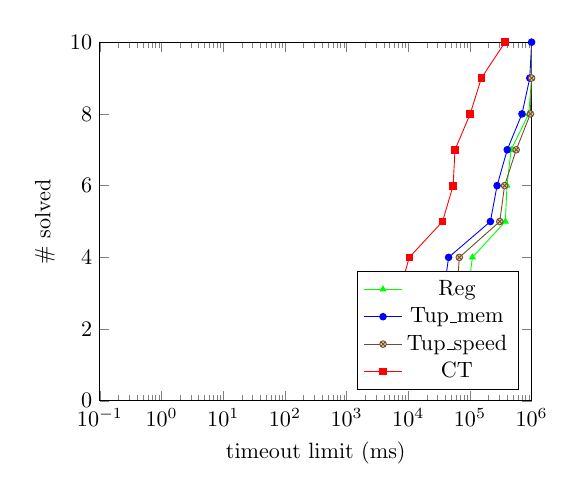
\begin{tikzpicture}[scale=0.8]
      \begin{axis}[
    xmode=log,
    ymin=0,ymax=10,
    xmin=0.1, xmax=1000000,
    every axis plot/.style={thin},
    xlabel={timeout limit (ms)},
    ylabel={\# solved},
    legend pos=south east
    % table/create on use/cumulative distribution/.style={
    %   create col/expr={\pgfmathaccuma + \thisrow{f(x)}}   
    % }
    ]
    \addplot 
    [mark=triangle*,
    mark size=1.5,
    mark options={solid},
    green] 
    coordinates {(31574.208, 1)
(89069.596, 2)
(92409.911, 3)
(109617.692, 4)
(375120.195, 5)
(398745.546, 6)
(464795.600, 7)
(896628.914, 8)
(1000000.519, 9)
(1000001.313, 10)};

    \addplot 
    [blue,
    mark=*,
    mark size=1.5,
    mark options={solid}]
    coordinates {(27237.714, 1)
(35441.131, 2)
(37441.293, 3)
(45077.352, 4)
(214515.372, 5)
(275244.504, 6)
(402643.388, 7)
(697541.797, 8)
(934131.437, 9)
(1000000.647, 10)};

    \addplot [brown!60!black,
    mark options={fill=brown!40},
    mark=otimes*,
    mark size=1.5]
    coordinates {(27847.614, 1)
(43395.528, 2)
(61320.788, 3)
(67245.864, 4)
(304719.299, 5)
(364282.419, 6)
(562899.918, 7)
(955072.437, 8)
(1000000.276, 9)
(1000185.158, 10)};

    \addplot 
    [red,
    mark size=1.5,
    mark=square*]
    coordinates {(4559.768, 1)
(5269.384, 2)
(7089.864, 3)
(10389.645, 4)
(35953.097, 5)
(53378.404, 6)
(57293.505, 7)
(100925.480, 8)
(153336.848, 9)
(371551.862, 10)};
    \legend{Reg,Tup\_mem,Tup\_speed,CT}
  \end{axis}

    \end{tikzpicture}
    \vfill
    \caption{\textbf{Rands JC5000.} The 10 instances of this benchmark
      contain constraints of arity 7. The variable domains are 0..7.}
    \label{fig:simple2}
    \vspace{\baselineskip}
  \end{minipage}\qquad

  \begin{minipage}[b][10cm][s]{.45\textwidth}
    \centering
    \vfill
    \begin{tikzpicture}[scale=0.8]
      \begin{tikzpicture}[scale=1.0]
  \begin{axis}[
    xmode=log,
    ymin=0,ymax=10,
    xmin=0.1, xmax=1000000,
    every axis plot/.style={thin},
    xlabel={timeout limit (ms)},
    ylabel={\# solved},
    legend pos=south east
    % table/create on use/cumulative distribution/.style={
    %   create col/expr={\pgfmathaccuma + \thisrow{f(x)}}   
    % }
    ]
    \addplot 
    [mark=triangle*,
    mark size=1.5,
    mark options={solid},
    green] 
    coordinates {139268.423 1
140601.911 2
177941.502 3
424666.930 4
1000000.472 5
1000000.888 6
1000001.221 7
1000001.407 8
1000001.457 9
1000003.369 10};

    \addplot 
    [blue,
    mark=*,
    mark size=1.5,
    mark options={solid}]
    coordinates {87932.493 1
117877.394 2
124316.924 3
273988.271 4
850622.333 5
1000000.839 6
1000001.004 7
1000001.005 8
1000001.889 9
1000002.453 10};

    \addplot [brown!60!black,
    mark options={fill=brown!40},
    mark=otimes*,
    mark size=1.5]
    table {122789.372 1
146789.073 2
167882.645 3
363255.524 4
1000000.384 5
1000001.258 6
1000002.593 7
1000002.808 8
1000003.164 9
1000004.253 10};

    \addplot 
    [red,
    mark size=1.5,
    mark=square*]
    table {11372.849 1
16562.793 2
18623.245 3
39394.203 4
121998.328 5
124778.898 6
201796.350 7
436664.869 8
954480.066 9
1000000.181 10};
    \legend{Reg,Tup\_mem,Tup\_speed,CT}
  \end{axis}
\end{tikzpicture}

    \end{tikzpicture}
    \vfill
    \caption{\textbf{Rands JC7500}. The 10 instances of this benchmark
      contain constraints of arity 7. The variable domains are 0..7.}
    \vspace{\baselineskip}
  \end{minipage}\qquad
  \begin{minipage}[b][10cm][s]{.45\textwidth}
    \centering
    \vfill
    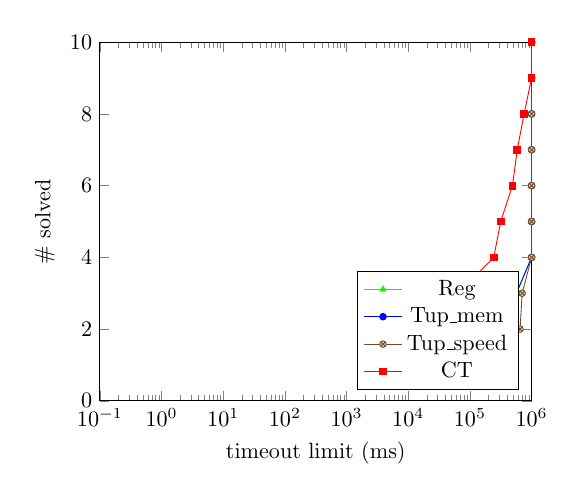
\begin{tikzpicture}[scale=0.8]
      \begin{axis}[
    xmode=log,
    ymin=0,ymax=10,
    xmin=0.1, xmax=1000000,
    every axis plot/.style={thin},
    xlabel={timeout limit (ms)},
    ylabel={\# solved},
    legend pos=south east
    % table/create on use/cumulative distribution/.style={
    %   create col/expr={\pgfmathaccuma + \thisrow{f(x)}}   
    % }
    ]
    \addplot 
    [mark=triangle*,
    mark size=1.5,
    mark options={solid},
    green] 
    coordinates {(332745.543, 1)
(523863.709, 2)
(569686.426, 3)
(1000000.172, 4)
(1000000.554, 5)
(1000000.920, 6)
(1000001.037, 7)
(1000001.490, 8)
(1000002.276, 9)
(1000003.312, 10)};

    \addplot 
    [blue,
    mark=*,
    mark size=1.5,
    mark options={solid}]
    coordinates {(226152.398, 1)
(491387.804, 2)
(566477.841, 3)
(1000000.822, 4)
(1000001.468, 5)
(1000001.597, 6)
(1000001.921, 7)
(1000002.047, 8)
(1000002.465, 9)
(1000003.238, 10)};

    \addplot [brown!60!black,
    mark options={fill=brown!40},
    mark=otimes*,
    mark size=1.5]
    coordinates {(294414.233, 1)
(649951.472, 2)
(702865.808, 3)
(1000000.517, 4)
(1000000.699, 5)
(1000000.802, 6)
(1000001.295, 7)
(1000001.350, 8)
(1000001.480, 9)
(1000001.637, 10)};

    \addplot 
    [red,
    mark size=1.5,
    mark=square*]
    coordinates {(25774.100, 1)
(57124.920, 2)
(64359.631, 3)
(243389.037, 4)
(315549.601, 5)
(489096.976, 6)
(584890.320, 7)
(755476.499, 8)
(1000000.186, 9)
(1000000.225, 10)};
    \legend{Reg,Tup\_mem,Tup\_speed,CT}
  \end{axis}

    \end{tikzpicture}
    \vfill
    \caption{\textbf{Rands JC10000}. The 10 instances of this benchmark
      contain constraints of arity 7. The variable domains are 0..7.}
    \vspace{\baselineskip}
  \end{minipage}\qquad

\end{figure}

\newpage

\begin{figure}
  
  \begin{minipage}[b][10cm][s]{0.45\textwidth}
    \centering
    \vfill
    \begin{tikzpicture}[scale=0.8]
      \begin{tikzpicture}[scale=1.0]
  \begin{axis}[
    xmode=log,
    ymin=0,ymax=23,
    xmin=0.1, xmax=1000000,
    every axis plot/.style={thin},
    xlabel={timeout limit (ms)},
    ylabel={\# solved},
    legend pos=south east
    % table/create on use/cumulative distribution/.style={
    %   create col/expr={\pgfmathaccuma + \thisrow{f(x)}}   
    % }
    ]
    \addplot 
    [mark=triangle*,
    mark size=1.5,
    mark options={solid},
    green] 
    coordinates {0.390 1
0.407 2
0.408 3
0.429 4
0.449 5
0.454 6
0.474 7
0.490 8
0.492 9
0.495 10
0.498 11
0.502 12
0.513 13
0.530 14
0.554 15
0.757 16
0.759 17
1.097 18
1.538 19
1.686 20
1.847 21
4.286 22
5.242 23};

    \addplot 
    [blue,
    mark=*,
    mark size=1.5,
    mark options={solid}]
    coordinates {0.431 1
0.706 2
0.742 3
0.771 4
1.021 5
1.885 6
1.911 7
2.208 8
3.074 9
3.167 10
4.797 11
11.430 12
19.852 13
62.120 14
72.766 15
90.320 16
191.654 17
227.574 18
297.702 19
497.460 20
2463.091 21
4400.894 22
7429.957 23};

    \addplot [brown!60!black,
    mark options={fill=brown!40},
    mark=otimes*,
    mark size=1.5]
    table {0.550 1
0.766 2
0.908 3
0.977 4
1.486 5
2.681 6
2.965 7
3.453 8
4.528 9
4.746 10
7.309 11
17.587 12
30.902 13
90.208 14
106.065 15
137.677 16
291.910 17
340.514 18
456.452 19
743.107 20
3772.207 21
6539.383 22
11517.655 23};

    \addplot 
    [red,
    mark size=1.5,
    mark=square*]
    table {0.439 1
0.618 2
0.698 3
0.735 4
1.093 5
1.910 6
2.099 7
2.368 8
2.794 9
3.010 10
4.795 11
11.303 12
19.709 13
53.169 14
61.288 15
66.296 16
156.013 17
182.439 18
253.668 19
338.968 20
1947.380 21
2773.622 22
4557.056 23};
    \legend{Reg,Tup\_mem,Tup\_speed,CT}
  \end{axis}
\end{tikzpicture}

    \end{tikzpicture}
    \vfill
    \caption{\textbf{AIM-50}. The 23 instances
    of this benchmark contain ternary constraints 
    and a few binary constraints. All variables
    are 0/1.}
    \vspace{\baselineskip}
  \end{minipage}\qquad
  \begin{minipage}[b][10cm][s]{0.45\textwidth}
    \centering
    \vfill
    \begin{tikzpicture}[scale=0.8]
      \begin{axis}[
    xmode=log,
    ymin=0,ymax=23,
    xmin=0.1, xmax=1000000,
    every axis plot/.style={thin},
    xlabel={timeout limit (ms)},
    ylabel={\# solved},
    legend pos=south east
    % table/create on use/cumulative distribution/.style={
    %   create col/expr={\pgfmathaccuma + \thisrow{f(x)}}   
    % }
    ]
    \addplot 
    [mark=triangle*,
    mark size=1.5,
    mark options={solid},
    green] 
    coordinates {(0.823, 1)
(0.832, 2)
(0.857, 3)
(0.867, 4)
(0.885, 5)
(0.918, 6)
(0.939, 7)
(0.953, 8)
(0.974, 9)
(0.981, 10)
(0.987, 11)
(0.988, 12)
(1.008, 13)
(1.061, 14)
(1.135, 15)
(1.205, 16)
(2.753, 17)
(3.647, 18)
(24.877, 19)
(24.886, 20)
(35.599, 21)
(42.011, 22)
(48.965, 23)};

    \addplot 
    [blue,
    mark=*,
    mark size=1.5,
    mark options={solid}]
    coordinates {(3.586, 1)
(3.671, 2)
(6.004, 3)
(9.450, 4)
(15.887, 5)
(52.426, 6)
(80.095, 7)
(171.902, 8)
(4436.194, 9)
(41949.006, 10)
(100934.221, 11)
(147492.566, 12)
(556004.535, 13)
(1000000.165, 14)
(1000000.167, 15)
(1000000.174, 16)
(1000000.174, 17)
(1000000.176, 18)
(1000000.179, 19)
(1000000.202, 20)
(1000000.260, 21)
(1000000.266, 22)
(1000000.286, 23)};

    \addplot [brown!60!black,
    mark options={fill=brown!40},
    mark=otimes*,
    mark size=1.5]
    table {(5.211, 1)
(5.793, 2)
(9.033, 3)
(13.782, 4)
(24.369, 5)
(77.669, 6)
(120.860, 7)
(258.984, 8)
(6933.488, 9)
(65101.206, 10)
(165079.465, 11)
(242773.103, 12)
(877436.255, 13)
(1000000.113, 14)
(1000000.118, 15)
(1000000.123, 16)
(1000000.132, 17)
(1000000.154, 18)
(1000000.165, 19)
(1000000.189, 20)
(1000000.191, 21)
(1000000.196, 22)
(1000000.259, 23)};

    \addplot 
    [red,
    mark size=1.5,
    mark=square*]
    table {(3.886, 1)
(4.643, 2)
(6.772, 3)
(11.080, 4)
(17.750, 5)
(62.656, 6)
(87.179, 7)
(187.117, 8)
(4632.128, 9)
(36310.893, 10)
(96431.551, 11)
(140762.037, 12)
(452408.039, 13)
(1000000.102, 14)
(1000000.115, 15)
(1000000.118, 16)
(1000000.134, 17)
(1000000.137, 18)
(1000000.157, 19)
(1000000.200, 20)
(1000000.202, 21)
(1000000.221, 22)
(1000000.239, 23)};
    \legend{Reg,Tup\_mem,Tup\_speed,CT}
  \end{axis}

    \end{tikzpicture}
    \vfill
    \caption{\textbf{AIM-100}. The 23 instances
      of this benchmark contain ternary constraints 
      and a few binary constraints. All variables
      are 0/1.}
    \vspace{\baselineskip}
  \end{minipage}\qquad
  \begin{minipage}[b][10cm][s]{0.45\textwidth}
    \centering
    \vfill
    \begin{tikzpicture}[scale=0.8]
      \begin{axis}[
    xmode=log,
    ymin=0,ymax=22,
    xmin=0.1, xmax=1000000,
    every axis plot/.style={thin},
    xlabel={timeout limit (ms)},
    ylabel={\# solved},
    legend pos=south east
    % table/create on use/cumulative distribution/.style={
    %   create col/expr={\pgfmathaccuma + \thisrow{f(x)}}   
    % }
    ]
    \addplot 
    [mark=triangle*,
    mark size=1.5,
    mark options={solid},
    green] 
    coordinates {(2.092, 1)
(2.153, 2)
(2.207, 3)
(2.224, 4)
(2.353, 5)
(2.410, 6)
(2.444, 7)
(2.462, 8)
(2.486, 9)
(2.626, 10)
(2.638, 11)
(4.751, 12)
(7.714, 13)
(12.349, 14)
(459.348, 15)
(786.654, 16)
(1926.845, 17)
(7178.726, 18)
(13920.549, 19)
(63961.995, 20)
(83629.587, 21)
(215920.851, 22)};

    \addplot 
    [blue,
    mark=*,
    mark size=1.5,
    mark options={solid}]
    coordinates {(92.762, 1)
(214.140, 2)
(5059.466, 3)
(9347.039, 4)
(1000000.212, 5)
(1000000.214, 6)
(1000000.230, 7)
(1000000.234, 8)
(1000000.236, 9)
(1000000.243, 10)
(1000000.247, 11)
(1000000.332, 12)
(1000000.348, 13)
(1000000.356, 14)
(1000000.384, 15)
(1000000.413, 16)
(1000000.580, 17)
(1001526.960, 18)
(1013587.491, 19)
(1015726.858, 20)
(1021700.000, 21)
(1026780.972, 22)};

    \addplot [brown!60!black,
    mark options={fill=brown!40},
    mark=otimes*,
    mark size=1.5]
    table {(144.623, 1)
(333.321, 2)
(9960.406, 3)
(14839.411, 4)
(1000000.132, 5)
(1000000.132, 6)
(1000000.138, 7)
(1000000.154, 8)
(1000000.156, 9)
(1000000.161, 10)
(1000000.176, 11)
(1000000.201, 12)
(1000000.233, 13)
(1000000.233, 14)
(1000000.264, 15)
(1000000.302, 16)
(1000000.338, 17)
(1000000.401, 18)
(1000000.462, 19)
(1000000.559, 20)
(1000201.313, 21)
(1030367.681, 22)};

    \addplot 
    [red,
    mark size=1.5,
    mark=square*]
    table {(120.173, 1)
(264.364, 2)
(6492.284, 3)
(12332.389, 4)
(1000000.117, 5)
(1000000.130, 6)
(1000000.138, 7)
(1000000.141, 8)
(1000000.144, 9)
(1000000.148, 10)
(1000000.157, 11)
(1000000.179, 12)
(1000000.199, 13)
(1000000.223, 14)
(1000000.258, 15)
(1000000.312, 16)
(1000000.349, 17)
(1000000.387, 18)
(1000000.408, 19)
(1019145.714, 20)
(1021004.571, 21)
(1051023.598, 22)};
    \legend{Reg,Tup\_mem,Tup\_speed,CT}
  \end{axis}

    \end{tikzpicture}
    \vfill
    \caption{\textbf{AIM-200}. The 22 instances
    of this benchmark contain contain ternary constraints 
    and a few binary constraints. All variables
    are 0/1.}
    \vspace{\baselineskip}
  \end{minipage}\qquad
\end{figure}

\newpage

\begin{figure}
  \begin{minipage}[b][10cm][s]{0.45\textwidth}
    \centering
    \vfill
    \begin{tikzpicture}[scale=0.8]
      \begin{tikzpicture}[scale=1.0]
  \begin{axis}[
    xmode=log,
    ymin=0,ymax=50,
    xmin=0.1, xmax=1000000,
    every axis plot/.style={thin},
    xlabel={timeout limit (ms)},
    ylabel={\# solved},
    legend pos=south east
    % table/create on use/cumulative distribution/.style={
    %   create col/expr={\pgfmathaccuma + \thisrow{f(x)}}   
    % }
    ]
    \addplot 
    [mark=triangle*,
    mark size=1.5,
    mark options={solid},
    green] 
    coordinates {21539.047 1
23631.895 2
23716.403 3
24241.194 4
24452.383 5
24702.581 6
24727.049 7
24735.421 8
24762.823 9
25381.219 10
25446.865 11
25447.244 12
25663.048 13
25681.411 14
25705.552 15
25921.922 16
26000.936 17
26206.810 18
26236.781 19
26242.879 20
26255.926 21
26263.647 22
26276.749 23
26572.969 24
26580.275 25
26658.352 26
26798.498 27
27134.428 28
27340.416 29
27401.714 30
27486.019 31
27561.142 32
27728.713 33
27922.916 34
28054.949 35
28057.644 36
28193.151 37
28328.067 38
28495.760 39
28577.913 40
28589.075 41
28945.618 42
29006.507 43
29341.039 44
29520.154 45
29560.978 46
29585.618 47
29688.054 48
29934.812 49
30055.889 50};

    \addplot 
    [blue,
    mark=*,
    mark size=1.5,
    mark options={solid}]
    coordinates {7672.186 1
7964.072 2
7988.188 3
8311.150 4
8326.644 5
8405.755 6
8413.912 7
8433.367 8
8543.205 9
8852.685 10
8991.001 11
9027.728 12
9120.668 13
9300.145 14
9307.344 15
9334.373 16
9427.760 17
9445.763 18
9469.390 19
9514.190 20
9600.928 21
9650.273 22
9746.749 23
9808.637 24
9817.477 25
9908.257 26
9966.772 27
9974.917 28
10107.698 29
10130.344 30
10214.500 31
10354.798 32
10411.441 33
10412.120 34
10566.980 35
10629.555 36
10690.029 37
10750.761 38
10771.949 39
10783.994 40
10796.075 41
10819.530 42
10910.396 43
10935.039 44
11189.948 45
11409.743 46
11725.089 47
11914.318 48
12087.322 49
12551.558 50};

    \addplot [brown!60!black,
    mark options={fill=brown!40},
    mark=otimes*,
    mark size=1.5]
    table {11083.294 1
11942.343 2
12057.186 3
12065.914 4
12165.546 5
12230.996 6
12353.178 7
12499.801 8
12539.423 9
12659.462 10
12724.767 11
12772.533 12
13125.773 13
13328.450 14
13638.694 15
13680.520 16
13726.853 17
13788.117 18
13799.316 19
13929.021 20
13937.426 21
14037.418 22
14066.707 23
14101.725 24
14130.306 25
14152.192 26
14478.238 27
14540.951 28
14544.138 29
14609.419 30
14697.861 31
14702.186 32
14899.661 33
15027.878 34
15089.663 35
15146.606 36
15213.444 37
15229.658 38
15372.915 39
15428.330 40
15796.160 41
15805.142 42
15904.232 43
16049.472 44
16141.290 45
16151.591 46
16160.955 47
16942.804 48
17001.615 49
17047.240 50};

    \addplot 
    [red,
    mark size=1.5,
    mark=square*]
    table {2427.974 1
2699.046 2
2717.750 3
2743.960 4
2797.776 5
2816.502 6
2841.334 7
2900.942 8
2904.804 9
2908.160 10
2910.491 11
2933.117 12
2933.400 13
2967.383 14
2989.519 15
3003.038 16
3029.964 17
3063.311 18
3093.973 19
3141.933 20
3150.100 21
3186.832 22
3220.475 23
3234.416 24
3239.493 25
3269.265 26
3293.108 27
3353.966 28
3379.302 29
3394.468 30
3439.955 31
3458.748 32
3527.174 33
3528.582 34
3540.231 35
3558.883 36
3570.218 37
3574.549 38
3610.825 39
3624.569 40
3627.753 41
3673.298 42
3729.990 43
3743.274 44
3779.422 45
3788.515 46
3859.838 47
3898.223 48
3979.624 49
4133.050 50};
    \legend{Reg,Tup\_mem,Tup\_speed,CT}
  \end{axis}
\end{tikzpicture}

    \end{tikzpicture}
    \vfill
    \caption{\textbf{A5}. The 50 instances
      of this benchmark contain constraints of arity 5.
      The variables are 0/1.}
    \vspace{\baselineskip}
  \end{minipage}\qquad

  \begin{minipage}[b][10cm][s]{0.45\textwidth}
    \centering
    \vfill
    \begin{tikzpicture}[scale=0.8]
      \begin{tikzpicture}[scale=1.0]
  \begin{axis}[
    xmode=log,
    ymin=0,ymax=23,
    xmin=0.1, xmax=1000000,
    every axis plot/.style={thin},
    xlabel={timeout limit (ms)},
    ylabel={\# solved},
    legend pos=south east
    % table/create on use/cumulative distribution/.style={
    %   create col/expr={\pgfmathaccuma + \thisrow{f(x)}}   
    % }
    ]
    \addplot 
    [mark=triangle*,
    mark size=1.5,
    mark options={solid},
    green] 
    coordinates {727435.433 1
1000001.373 2
1000005.483 3
1000006.809 4
1000008.096 5
1000009.635 6
1000010.074 7
1000011.271 8
1000012.432 9
1000012.672 10
1000015.905 11
1000017.026 12
1000022.231 13
1000029.449 14
1000030.270 15
1000031.062 16
1000036.397 17
1000036.748 18
1000039.103 19
1000043.823 20
1000044.070 21
1000052.767 22
1000080.677 23};

    \addplot 
    [blue,
    mark=*,
    mark size=1.5,
    mark options={solid}]
    coordinates {224520.942 1
311434.541 2
518531.192 3
563843.176 4
816767.503 5
1000001.025 6
1000001.573 7
1000003.413 8
1000003.543 9
1000003.636 10
1000004.219 11
1000005.825 12
1000006.947 13
1000008.010 14
1000009.980 15
1000012.435 16
1000015.261 17
1000015.833 18
1000017.025 19
1000023.640 20
1000029.233 21
1000041.787 22
1000054.453 23};

    \addplot [brown!60!black,
    mark options={fill=brown!40},
    mark=otimes*,
    mark size=1.5]
    table {316710.534 1
410461.377 2
648720.274 3
713048.102 4
1000002.616 5
1000004.304 6
1000005.477 7
1000005.720 8
1000009.313 9
1000010.227 10
1000014.478 11
1000014.751 12
1000020.934 13
1000021.694 14
1000022.834 15
1000022.849 16
1000028.045 17
1000028.187 18
1000031.847 19
1000032.588 20
1000032.896 21
1000044.704 22
1000046.876 23};

    \addplot 
    [red,
    mark size=1.5,
    mark=square*]
    table {20486.588 1
58503.164 2
61130.226 3
77146.092 4
94763.488 5
153385.993 6
226208.408 7
402373.676 8
417665.968 9
446212.851 10
455410.096 11
600725.556 12
1000000.185 13
1000000.197 14
1000000.502 15
1000000.985 16
1000001.080 17
1000001.500 18
1000001.515 19
1000001.657 20
1000002.297 21
1000002.778 22
1000003.801 23};
    \legend{Reg,Tup\_mem,Tup\_speed,CT}
  \end{axis}
\end{tikzpicture}

    \end{tikzpicture}
    \vfill
    \caption{\textbf{A10}. The 50 instances
    of this benchmark contain constraints of arity X.
    Most of the variables are 0/1, and some are
    singletons.}
    \vspace{\baselineskip}
  \end{minipage}\qquad
\end{figure}

\newpage

\begin{figure}
  \begin{minipage}[b][10cm][s]{0.45\textwidth}
    \centering
    \vfill
    \begin{tikzpicture}[scale=0.8]
      \begin{tikzpicture}[scale=1.0]
  \begin{axis}[
    xmode=log,
    ymin=0,ymax=65,
    xmin=0.1, xmax=1000000,
    every axis plot/.style={thin},
    xlabel={timeout limit (ms)},
    ylabel={\# solved},
    legend pos=south east
    % table/create on use/cumulative distribution/.style={
    %   create col/expr={\pgfmathaccuma + \thisrow{f(x)}}   
    % }
    ]
    \addplot 
    [mark=triangle*,
    mark size=1.5,
    mark options={solid},
    green] 
    coordinates {0.078 1
0.089 2
0.089 3
0.093 4
0.094 5
0.095 6
0.095 7
0.097 8
0.098 9
0.098 10
0.099 11
0.099 12
0.099 13
0.102 14
0.103 15
0.103 16
0.106 17
0.157 18
0.831 19
1.490 20
1.498 21
1.518 22
1.954 23
3.734 24
3.737 25
4.347 26
9.191 27
10.580 28
19.169 29
22.780 30
26.266 31
81.558 32
102.447 33
104.991 34
131.512 35
332.462 36
352.388 37
618.827 38
788.523 39
790.494 40
1259.350 41
1678.432 42
1862.544 43
2455.933 44
2837.051 45
3271.878 46
4855.913 47
6934.464 48
7463.727 49
8049.052 50
8952.593 51
19737.517 52
23132.443 53
23469.266 54
26002.371 55
29111.360 56
42946.710 57
73225.089 58
74320.226 59
75593.251 60
108672.990 61
122929.922 62
149958.110 63
163565.715 64
261688.209 65};

    \addplot 
    [blue,
    mark=*,
    mark size=1.5,
    mark options={solid}]
    coordinates {0.342 1
0.351 2
0.361 3
0.400 4
0.401 5
0.420 6
0.433 7
0.433 8
0.436 9
0.442 10
0.476 11
0.489 12
0.492 13
0.493 14
0.549 15
0.590 16
0.652 17
0.720 18
0.923 19
1.008 20
1.184 21
1.528 22
1.727 23
2.724 24
3.600 25
7.208 26
7.829 27
8.978 28
12.102 29
17.784 30
33.887 31
40.219 32
55.846 33
61.501 34
164.731 35
184.236 36
360.816 37
429.133 38
484.976 39
586.591 40
794.649 41
932.019 42
1474.042 43
1555.417 44
1890.818 45
3795.101 46
5347.478 47
6026.047 48
7463.682 49
9392.594 50
12105.731 51
25050.002 52
40536.372 53
48045.798 54
61824.891 55
74212.070 56
143995.198 57
243803.619 58
296870.468 59
302900.312 60
322459.873 61
333997.695 62
444619.255 63
457064.862 64
908177.605 65};

    \addplot [brown!60!black,
    mark options={fill=brown!40},
    mark=otimes*,
    mark size=1.5]
    table {0.702 1
0.797 2
0.808 3
0.911 4
0.944 5
0.954 6
0.961 7
1.001 8
1.027 9
1.096 10
1.103 11
1.108 12
1.156 13
1.178 14
1.190 15
1.198 16
1.218 17
1.346 18
1.419 19
1.807 20
2.596 21
3.899 22
4.099 23
5.733 24
5.889 25
9.553 26
10.532 27
11.796 28
28.281 29
29.933 30
49.328 31
75.166 32
103.942 33
120.948 34
278.999 35
367.701 36
427.636 37
574.683 38
660.416 39
802.131 40
1091.373 41
1360.532 42
1932.804 43
2291.232 44
2682.220 45
5395.569 46
7382.573 47
8090.518 48
8788.504 49
12047.370 50
15892.962 51
30283.964 52
52697.241 53
60018.686 54
76459.238 55
87041.593 56
184487.102 57
286328.868 58
338304.442 59
353888.532 60
366508.306 61
398389.231 62
531168.118 63
545050.662 64
1000001.713 65};

    \addplot 
    [red,
    mark size=1.5,
    mark=square*]
    table {0.069 1
0.069 2
0.080 3
0.086 4
0.086 5
0.089 6
0.089 7
0.089 8
0.090 9
0.091 10
0.092 11
0.092 12
0.093 13
0.093 14
0.094 15
0.096 16
0.099 17
0.101 18
0.365 19
0.406 20
0.422 21
0.510 22
0.784 23
1.236 24
1.591 25
1.712 26
1.824 27
2.622 28
5.997 29
6.538 30
7.745 31
17.398 32
24.309 33
26.727 34
33.697 35
63.005 36
63.138 37
77.013 38
147.914 39
162.476 40
176.882 41
296.947 42
330.613 43
459.449 44
472.783 45
804.999 46
1061.529 47
1140.902 48
1254.905 49
1867.303 50
2462.669 51
4400.046 52
8169.387 53
9165.590 54
9457.464 55
9850.643 56
23517.073 57
36089.500 58
38817.645 59
40027.459 60
47404.529 61
50511.047 62
64207.992 63
70129.605 64
130009.590 65};
    \legend{Reg,Tup\_mem,Tup\_speed,CT}
  \end{axis}
\end{tikzpicture}

    \end{tikzpicture}
    \vfill
    \caption{\textbf{Crosswords WorldVG}.
    The 65 instances of this benchmark contain 
    constraints of arities ranging from 2 to 20. 
    The variable domains are 0..25.}
    \vspace{\baselineskip}
  \end{minipage}\qquad

    \begin{minipage}[b][10cm][s]{0.45\textwidth}
    \centering
    \vfill
    \begin{tikzpicture}[scale=0.8]
      \begin{axis}[
    xmode=log,
    ymin=0,ymax=63,
    xmin=0.1, xmax=1000000,
    every axis plot/.style={thin},
    xlabel={timeout limit (ms)},
    ylabel={\# solved},
    legend pos=south east
    % table/create on use/cumulative distribution/.style={
    %   create col/expr={\pgfmathaccuma + \thisrow{f(x)}}   
    % }
    ]
    \addplot 
    [mark=triangle*,
    mark size=1.5,
    mark options={solid},
    green] 
    coordinates {(0.074, 1)
(0.076, 2)
(0.078, 3)
(0.082, 4)
(0.089, 5)
(0.089, 6)
(0.092, 7)
(0.096, 8)
(0.097, 9)
(0.097, 10)
(0.097, 11)
(0.099, 12)
(0.099, 13)
(0.102, 14)
(0.103, 15)
(0.108, 16)
(0.117, 17)
(0.123, 18)
(0.500, 19)
(0.676, 20)
(0.723, 21)
(0.905, 22)
(1.332, 23)
(1.692, 24)
(1.766, 25)
(1.791, 26)
(5.276, 27)
(16.858, 28)
(17.927, 29)
(30.069, 30)
(35.255, 31)
(41.801, 32)
(52.490, 33)
(75.080, 34)
(96.307, 35)
(130.683, 36)
(131.067, 37)
(225.774, 38)
(274.112, 39)
(379.638, 40)
(550.637, 41)
(909.264, 42)
(1274.166, 43)
(1388.373, 44)
(2525.152, 45)
(2533.498, 46)
(2595.853, 47)
(4030.753, 48)
(4547.362, 49)
(5055.465, 50)
(5791.415, 51)
(10242.753, 52)
(12298.425, 53)
(14360.436, 54)
(14982.830, 55)
(17458.388, 56)
(20992.013, 57)
(29908.599, 58)
(33944.527, 59)
(36060.331, 60)
(55002.467, 61)
(60672.239, 62)
(76112.252, 63)};

    \addplot 
    [blue,
    mark=*,
    mark size=1.5,
    mark options={solid}]
    coordinates {(0.273, 1)
(0.276, 2)
(0.280, 3)
(0.282, 4)
(0.283, 5)
(0.284, 6)
(0.299, 7)
(0.306, 8)
(0.311, 9)
(0.319, 10)
(0.323, 11)
(0.345, 12)
(0.352, 13)
(0.399, 14)
(0.502, 15)
(0.503, 16)
(0.531, 17)
(0.536, 18)
(0.570, 19)
(0.573, 20)
(0.880, 21)
(1.282, 22)
(1.284, 23)
(1.298, 24)
(1.740, 25)
(2.601, 26)
(3.676, 27)
(4.898, 28)
(9.614, 29)
(9.646, 30)
(17.588, 31)
(26.301, 32)
(53.031, 33)
(63.457, 34)
(140.413, 35)
(155.119, 36)
(167.139, 37)
(223.250, 38)
(272.924, 39)
(302.082, 40)
(761.487, 41)
(945.499, 42)
(1346.690, 43)
(1449.372, 44)
(1491.881, 45)
(2704.616, 46)
(3119.614, 47)
(5009.739, 48)
(5632.408, 49)
(7755.518, 50)
(8079.373, 51)
(13953.623, 52)
(17063.131, 53)
(19618.816, 54)
(21960.324, 55)
(24240.394, 56)
(39633.214, 57)
(64699.544, 58)
(71580.728, 59)
(73166.699, 60)
(112247.995, 61)
(121257.043, 62)
(151915.668, 63)};

    \addplot [brown!60!black,
    mark options={fill=brown!40},
    mark=otimes*,
    mark size=1.5]
    table {(0.412, 1)
(0.457, 2)
(0.458, 3)
(0.464, 4)
(0.471, 5)
(0.484, 6)
(0.496, 7)
(0.516, 8)
(0.572, 9)
(0.572, 10)
(0.598, 11)
(0.679, 12)
(0.734, 13)
(0.864, 14)
(1.027, 15)
(1.106, 16)
(1.203, 17)
(1.280, 18)
(1.557, 19)
(1.667, 20)
(2.002, 21)
(2.016, 22)
(2.303, 23)
(2.819, 24)
(2.952, 25)
(2.970, 26)
(5.162, 27)
(5.506, 28)
(18.023, 29)
(19.081, 30)
(39.969, 31)
(56.794, 32)
(100.167, 33)
(128.098, 34)
(172.182, 35)
(249.519, 36)
(259.430, 37)
(286.138, 38)
(488.848, 39)
(568.244, 40)
(1062.970, 41)
(1350.822, 42)
(1626.744, 43)
(1729.003, 44)
(2145.034, 45)
(3496.611, 46)
(3833.896, 47)
(6131.314, 48)
(7395.849, 49)
(9657.251, 50)
(10635.431, 51)
(17957.948, 52)
(19794.735, 53)
(25594.928, 54)
(27375.416, 55)
(30057.643, 56)
(50552.660, 57)
(78826.698, 58)
(88585.449, 59)
(90256.706, 60)
(134279.170, 61)
(143593.547, 62)
(181192.715, 63)};

    \addplot 
    [red,
    mark size=1.5,
    mark=square*]
    table {(0.068, 1)
(0.068, 2)
(0.069, 3)
(0.070, 4)
(0.072, 5)
(0.073, 6)
(0.073, 7)
(0.075, 8)
(0.077, 9)
(0.080, 10)
(0.081, 11)
(0.084, 12)
(0.087, 13)
(0.087, 14)
(0.088, 15)
(0.088, 16)
(0.089, 17)
(0.090, 18)
(0.091, 19)
(0.093, 20)
(0.350, 21)
(0.416, 22)
(0.568, 23)
(0.568, 24)
(0.626, 25)
(0.803, 26)
(1.154, 27)
(1.608, 28)
(4.334, 29)
(4.592, 30)
(9.543, 31)
(14.146, 32)
(20.935, 33)
(24.430, 34)
(31.227, 35)
(39.168, 36)
(59.321, 37)
(71.346, 38)
(116.614, 39)
(120.688, 40)
(172.687, 41)
(207.521, 42)
(217.931, 43)
(266.423, 44)
(477.466, 45)
(566.003, 46)
(683.586, 47)
(1064.142, 48)
(1232.853, 49)
(1672.169, 50)
(1747.561, 51)
(2681.469, 52)
(2811.215, 53)
(4092.535, 54)
(4387.910, 55)
(5269.595, 56)
(8047.345, 57)
(14122.235, 58)
(14686.169, 59)
(14970.167, 60)
(19502.734, 61)
(26550.723, 62)
(32323.306, 63)};
    \legend{Reg,Tup\_mem,Tup\_speed,CT}
  \end{axis}

    \end{tikzpicture}
    \vfill
    \caption{\textbf{Crosswords LexVG}.
    The 63 instances of this benchmark contain
    constraints of arity from 5 to 20. 
    Variable domains are 0..25.}
    \vspace{\baselineskip}
  \end{minipage}\qquad
  \begin{minipage}[b][10cm][s]{0.45\textwidth}
    \centering
    \vfill
    \begin{tikzpicture}[scale=0.8]
      \begin{tikzpicture}[scale=1.0]
  \begin{axis}[
    xmode=log,
    ymin=0,ymax=22,
    xmin=0.1, xmax=1000000,
    every axis plot/.style={thin},
    xlabel={timeout limit (ms)},
    ylabel={\# solved},
    legend pos=south east
    % table/create on use/cumulative distribution/.style={
    %   create col/expr={\pgfmathaccuma + \thisrow{f(x)}}   
    % }
    ]
    \addplot 
    [mark=triangle*,
    mark size=1.5,
    mark options={solid},
    green] 
    coordinates {0.150 1
0.382 2
1.156 3
1.231 4
1.662 5
1.826 6
2.291 7
2.622 8
5.011 9
8.353 10
9.860 11
15.302 12
18.579 13
22.834 14
27.862 15
29.816 16
36.345 17
45.878 18
285.224 19
1131.791 20
1278.079 21
2204.696 22};

    \addplot 
    [blue,
    mark=*,
    mark size=1.5,
    mark options={solid}]
    coordinates {0.138 1
0.311 2
0.790 3
1.624 4
1.760 5
1.791 6
2.063 7
3.631 8
4.094 9
4.213 10
5.035 11
5.357 12
6.556 13
6.847 14
9.371 15
11.612 16
16.633 17
18.028 18
42.410 19
175.300 20
4664.842 21
193998.166 22};

    \addplot [brown!60!black,
    mark options={fill=brown!40},
    mark=otimes*,
    mark size=1.5]
    table {0.146 1
0.391 2
0.855 3
1.897 4
1.958 5
2.033 6
2.272 7
4.342 8
4.459 9
4.946 10
5.389 11
5.697 12
7.018 13
7.259 14
10.784 15
12.976 16
20.478 17
20.679 18
41.775 19
49.515 20
218.327 21
246737.472 22};

    \addplot 
    [red,
    mark size=1.5,
    mark=square*]
    table {0.125 1
0.237 2
0.372 3
0.544 4
0.636 5
0.682 6
0.685 7
1.085 8
1.099 9
1.110 10
1.455 11
1.631 12
1.870 13
2.270 14
3.062 15
4.409 16
8.078 17
8.255 18
18.086 19
20.971 20
61.702 21
127890.223 22};
    \legend{Reg,Tup\_mem,Tup\_speed,CT}
  \end{axis}
\end{tikzpicture}

    \end{tikzpicture}
    \vfill
    \caption{\textbf{Crosswords Wordspuzzle}.
      The 22 instances of this benchmark contain 
      constraints of arities ranging from 2 to 13.
      The variable domains are 0..25.}
    \vspace{\baselineskip}
  \end{minipage}\qquad
  
\end{figure}

\newpage

\begin{figure}
    \begin{minipage}[b][10cm][s]{0.45\textwidth}
    \centering
    \vfill
    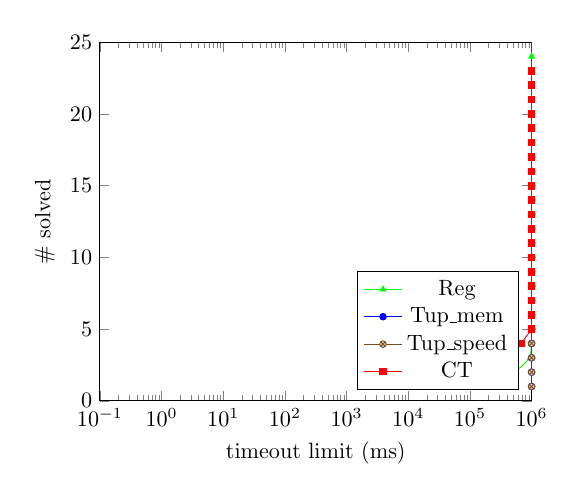
\begin{tikzpicture}[scale=0.8]
      \begin{axis}[
    xmode=log,
    ymin=0,ymax=25,
    xmin=0.1, xmax=1000000,
    every axis plot/.style={thin},
    xlabel={timeout limit (ms)},
    ylabel={\# solved},
    legend pos=south east
    % table/create on use/cumulative distribution/.style={
    %   create col/expr={\pgfmathaccuma + \thisrow{f(x)}}   
    % }
    ]
    \addplot 
    [mark=triangle*,
    mark size=1.5,
    mark options={solid},
    green] 
    coordinates {(362179.365, 1)
(542610.443, 2)
(956273.144, 3)
(1000000.188, 4)
(1000000.201, 5)
(1000000.201, 6)
(1000000.220, 7)
(1000000.266, 8)
(1000000.268, 9)
(1000000.291, 10)
(1000000.294, 11)
(1000000.295, 12)
(1000000.297, 13)
(1000000.329, 14)
(1000000.339, 15)
(1000000.376, 16)
(1000000.377, 17)
(1000000.409, 18)
(1000000.412, 19)
(1000000.463, 20)
(1000000.483, 21)
(1000000.641, 22)
(1000000.668, 23)
(1000000.801, 24)
(1029699.464, 25)};

    \addplot 
    [blue,
    mark=*,
    mark size=1.5,
    mark options={solid}]
    coordinates {(1000001.069, 1)
(1000001.150, 2)
(1000001.274, 3)
(1000001.277, 4)
(1000001.523, 5)
(1000002.056, 6)
(1000002.073, 7)
(1000002.311, 8)
(1000002.579, 9)
(1000002.756, 10)
(1000003.085, 11)
(1000004.834, 12)
(1000004.876, 13)
(1000005.836, 14)
(1000005.855, 15)
(1000006.115, 16)
(1000006.863, 17)
(1000007.924, 18)
(1000008.395, 19)
(1000008.443, 20)
(1000009.040, 21)
(1000013.352, 22)
(1000013.437, 23)
(1000013.463, 24)
(1022769.751, 25)};

    \addplot [brown!60!black,
    mark options={fill=brown!40},
    mark=otimes*,
    mark size=1.5]
    coordinates {(1000000.597, 1)
(1000000.598, 2)
(1000000.770, 3)
(1000000.849, 4)
(1000001.124, 5)
(1000001.175, 6)
(1000001.309, 7)
(1000001.317, 8)
(1000001.461, 9)
(1000001.753, 10)
(1000001.826, 11)
(1000002.114, 12)
(1000002.685, 13)
(1000003.527, 14)
(1000003.580, 15)
(1000003.656, 16)
(1000004.416, 17)
(1000005.342, 18)
(1000006.111, 19)
(1000006.504, 20)
(1000007.848, 21)
(1000009.651, 22)
(1000010.626, 23)
(1000011.794, 24)
(1000016.468, 25)};

    \addplot 
    [red,
    mark size=1.5,
    mark=square*]
    coordinates {(45570.744, 1)
(97963.633, 2)
(284803.058, 3)
(676940.142, 4)
(1000000.180, 5)
(1000000.233, 6)
(1000000.268, 7)
(1000000.271, 8)
(1000000.295, 9)
(1000000.309, 10)
(1000000.312, 11)
(1000000.324, 12)
(1000000.334, 13)
(1000000.347, 14)
(1000000.351, 15)
(1000000.363, 16)
(1000000.386, 17)
(1000000.400, 18)
(1000000.453, 19)
(1000000.503, 20)
(1000000.579, 21)
(1000000.609, 22)
(1000000.673, 23)
(1019921.469, 24)
(1040148.010, 25)};
    \legend{Reg,Tup\_mem,Tup\_speed,CT}
  \end{axis}

    \end{tikzpicture}
    \vfill
    \caption{\textbf{MDD 05}. The 25 instances of this benchmark
    contain constraints of arity $7$. The variable domains
    are 0..4.}
    \vspace{\baselineskip}
  \end{minipage}\qquad
  \begin{minipage}[b][10cm][s]{0.45\textwidth}
    \centering
    \vfill
    \begin{tikzpicture}[scale=0.8]
      \begin{tikzpicture}[scale=1.0]
  \begin{axis}[
    xmode=log,
    ymin=0,ymax=9,
    xmin=0.1, xmax=1000000,
    every axis plot/.style={thin},
    xlabel={timeout limit (ms)},
    ylabel={\# solved},
    legend pos=south east
    % table/create on use/cumulative distribution/.style={
    %   create col/expr={\pgfmathaccuma + \thisrow{f(x)}}   
    % }
    ]
    \addplot 
    [mark=triangle*,
    mark size=1.5,
    mark options={solid},
    green] 
    coordinates {8143.453 1
28227.868 2
30184.398 3
39636.695 4
40458.753 5
56228.579 6
66820.027 7
79866.961 8
245383.866 9};

    \addplot 
    [blue,
    mark=*,
    mark size=1.5,
    mark options={solid}]
    coordinates {1000001.471 1
1000001.544 2
1000002.625 3
1000002.721 4
1000002.899 5
1000003.208 6
1000004.208 7
1000004.650 8
1000005.052 9};

    \addplot [brown!60!black,
    mark options={fill=brown!40},
    mark=otimes*,
    mark size=1.5]
    table {1000000.498 1
1000000.780 2
1000000.821 3
1000001.078 4
1000001.299 5
1000001.505 6
1000002.168 7
1000004.073 8
1000008.854 9};

    \addplot 
    [red,
    mark size=1.5,
    mark=square*]
    table {1000000.160 1
1000000.224 2
1000000.247 3
1000000.259 4
1000000.300 5
1000000.307 6
1000000.343 7
1000000.404 8
1000000.445 9};
    \legend{Reg,Tup\_mem,Tup\_speed,CT}
  \end{axis}
\end{tikzpicture}

    \end{tikzpicture}
    \vfill
    \caption{\textbf{MDD 07}. The 9 instances of this benchmark
    contain constraints of arity $7$. The variable domains are
    0..4.}
    \vspace{\baselineskip}
  \end{minipage}\qquad
  \begin{minipage}[b][10cm][s]{.45\textwidth}
    \centering
    \vfill
    \begin{tikzpicture}[scale=0.8]
      \begin{tikzpicture}[scale=1.0]
  \begin{axis}[
    xmode=log,
    ymin=0,ymax=18,
    xmin=0.1, xmax=1000000,
    every axis plot/.style={thin},
    xlabel={timeout limit (ms)},
    ylabel={\# solved},
    legend pos=south east
    % table/create on use/cumulative distribution/.style={
    %   create col/expr={\pgfmathaccuma + \thisrow{f(x)}}   
    % }
    ]
    \addplot 
    [mark=triangle*,
    mark size=1.5,
    mark options={solid},
    green] 
    coordinates {160.082 1
199.047 2
738.646 3
1073.574 4
1941.132 5
4192.527 6
160.082 1
199.047 2
738.646 3
1073.574 4
1941.132 5
4192.527 6
(160.082,1)
(199.047,2)
(738.646,3)
(1073.574,4)
(1941.132,5)
(4192.527,6)};

    \addplot 
    [blue,
    mark=*,
    mark size=1.5,
    mark options={solid}]
    coordinates {1000001.385 1
1015679.482 2
1016279.242 3
1016406.246 4
1031535.613 5
1048711.823 6
1000001.385 1
1015679.482 2
1016279.242 3
1016406.246 4
1031535.613 5
1048711.823 6
(1000001.385,1)
(1015679.482,2)
(1016279.242,3)
(1016406.246,4)
(1031535.613,5)
(1048711.823,6)};

    \addplot [brown!60!black,
    mark options={fill=brown!40},
    mark=otimes*,
    mark size=1.5]
    table {1000000.720 1
1000001.967 2
1000005.371 3
1005327.065 4
1007653.014 5
1014601.258 6
1000000.720 1
1000001.967 2
1000005.371 3
1005327.065 4
1007653.014 5
1014601.258 6
(1000000.720,1)
(1000001.967,2)
(1000005.371,3)
(1005327.065,4)
(1007653.014,5)
(1014601.258,6)};

    \addplot 
    [red,
    mark size=1.5,
    mark=square*]
    table {1000000.477 1
1000881.615 2
1008283.620 3
1017720.801 4
1023341.972 5
1037219.927 6
1000000.477 1
1000881.615 2
1008283.620 3
1017720.801 4
1023341.972 5
1037219.927 6
(1000000.477,1)
(1000881.615,2)
(1008283.620,3)
(1017720.801,4)
(1023341.972,5)
(1037219.927,6)};
    \legend{Reg,Tup\_mem,Tup\_speed,CT}
  \end{axis}
\end{tikzpicture}

    \end{tikzpicture}
    \vfill
    \caption{\textbf{MDD 09}. The 10 instances of this benchmark
    contain constraints of arity $7$. The variable domains are
  0..4.}
    \vspace{\baselineskip}
  \end{minipage}\qquad
\end{figure}

\newpage

\begin{figure}
  \begin{minipage}[b][10cm][s]{0.45\textwidth}
    \centering
    \vfill
    \begin{tikzpicture}[scale=0.8]
      \begin{tikzpicture}[scale=1.0]
  \begin{axis}[
    xmode=log,
    ymin=0,ymax=314,
    xmin=0.1, xmax=1000000,
    every axis plot/.style={thin},
    xlabel={timeout limit (ms)},
    ylabel={\# solved},
    legend pos=south east
    % table/create on use/cumulative distribution/.style={
    %   create col/expr={\pgfmathaccuma + \thisrow{f(x)}}   
    % }
    ]
    \addplot 
    [mark=triangle*,
    mark size=1.5,
    mark options={solid},
    green] 
    table {./instances/kakuroext_easy/reg.data};

    \addplot 
    [blue,
    mark=*,
    mark size=1.5,
    mark options={solid}]
    table {./instances/kakuroext_easy/tup_mem.data};

    \addplot [brown!60!black,
    mark options={fill=brown!40},
    mark=otimes*,
    mark size=1.5]
    table {./instances/kakuroext_easy/tup_speed.data};

    \addplot 
    [red,
    mark size=1.5,
    mark=square*]
    table {./instances/kakuroext_easy/ct.data};
    \legend{Reg,Tup\_mem,Tup\_speed,CT}
  \end{axis}
\end{tikzpicture}

    \end{tikzpicture}
    \vfill
    \caption{\textbf{Kakuro easy}. The 172 instances
    of this benchmark contain constraints of arity varying
    from $2$ to $9$.
    The variable domains are 1..9.}
    \vspace{\baselineskip}
  \end{minipage}\qquad

  \begin{minipage}[b][10cm][s]{0.45\textwidth}
    \centering
    \vfill
    \begin{tikzpicture}[scale=0.8]
      \begin{axis}[
    xmode=log,
    ymin=0,ymax=163,
    xmin=0.1, xmax=1000000,
    every axis plot/.style={thin},
    xlabel={timeout limit (ms)},
    ylabel={\# solved},
    legend pos=south east
    % table/create on use/cumulative distribution/.style={
    %   create col/expr={\pgfmathaccuma + \thisrow{f(x)}}   
    % }
    ]
    \addplot 
    [mark=triangle*,
    mark size=1.5,
    mark options={solid},
    green] 
    coordinates {(0.292, 1)
(0.366, 2)
(0.373, 3)
(0.375, 4)
(0.377, 5)
(0.388, 6)
(0.389, 7)
(0.390, 8)
(0.395, 9)
(0.395, 10)
(0.397, 11)
(0.398, 12)
(0.405, 13)
(0.406, 14)
(0.406, 15)
(0.409, 16)
(0.411, 17)
(0.413, 18)
(0.416, 19)
(0.420, 20)
(0.429, 21)
(0.442, 22)
(0.446, 23)
(0.449, 24)
(0.450, 25)
(0.453, 26)
(0.454, 27)
(0.457, 28)
(0.461, 29)
(0.462, 30)
(0.462, 31)
(0.465, 32)
(0.475, 33)
(0.479, 34)
(0.483, 35)
(0.498, 36)
(0.518, 37)
(0.526, 38)
(0.532, 39)
(0.533, 40)
(0.569, 41)
(0.606, 42)
(0.615, 43)
(0.619, 44)
(0.620, 45)
(0.627, 46)
(0.628, 47)
(0.639, 48)
(0.647, 49)
(0.652, 50)
(0.655, 51)
(0.655, 52)
(0.660, 53)
(0.667, 54)
(0.670, 55)
(0.671, 56)
(0.672, 57)
(0.676, 58)
(0.678, 59)
(0.682, 60)
(0.690, 61)
(0.696, 62)
(0.697, 63)
(0.699, 64)
(0.705, 65)
(0.706, 66)
(0.714, 67)
(0.721, 68)
(0.724, 69)
(0.724, 70)
(0.725, 71)
(0.729, 72)
(0.729, 73)
(0.739, 74)
(0.740, 75)
(0.752, 76)
(0.755, 77)
(0.756, 78)
(0.762, 79)
(0.764, 80)
(0.765, 81)
(0.770, 82)
(0.773, 83)
(0.776, 84)
(0.778, 85)
(0.781, 86)
(0.782, 87)
(0.784, 88)
(0.791, 89)
(0.792, 90)
(0.792, 91)
(0.795, 92)
(0.798, 93)
(0.809, 94)
(0.811, 95)
(0.818, 96)
(0.840, 97)
(0.843, 98)
(0.850, 99)
(0.865, 100)
(0.875, 101)
(0.876, 102)
(0.879, 103)
(0.883, 104)
(0.919, 105)
(0.946, 106)
(0.956, 107)
(0.973, 108)
(0.982, 109)
(0.991, 110)
(0.993, 111)
(1.013, 112)
(1.028, 113)
(1.128, 114)
(1.220, 115)
(1.629, 116)
(1.937, 117)
(1.984, 118)
(2.002, 119)
(2.141, 120)
(2.188, 121)
(2.223, 122)
(2.373, 123)
(2.728, 124)
(6.575, 125)
(16.845, 126)
(16.868, 127)
(17.495, 128)
(20.180, 129)
(47.620, 130)
(55.482, 131)
(67.498, 132)
(67.776, 133)
(155.334, 134)
(156.640, 135)
(167.546, 136)
(172.809, 137)
(196.818, 138)
(204.653, 139)
(204.863, 140)
(217.964, 141)
(329.079, 142)
(389.985, 143)
(407.197, 144)
(523.926, 145)
(697.290, 146)
(887.001, 147)
(898.340, 148)
(1081.375, 149)
(1084.068, 150)
(1174.012, 151)
(1425.046, 152)
(1584.244, 153)
(1628.143, 154)
(1868.481, 155)
(2070.450, 156)
(2163.404, 157)
(2425.521, 158)
(2641.938, 159)
(7228.341, 160)
(7393.205, 161)
(7834.491, 162)
(13216.356, 163)};

    \addplot 
    [blue,
    mark=*,
    mark size=1.5,
    mark options={solid}]
    coordinates {(0.242, 1)
(0.303, 2)
(0.419, 3)
(0.438, 4)
(0.452, 5)
(0.458, 6)
(0.461, 7)
(0.465, 8)
(0.490, 9)
(0.493, 10)
(0.494, 11)
(0.494, 12)
(0.498, 13)
(0.503, 14)
(0.508, 15)
(0.516, 16)
(0.517, 17)
(0.538, 18)
(0.542, 19)
(0.551, 20)
(0.552, 21)
(0.565, 22)
(0.566, 23)
(0.586, 24)
(0.590, 25)
(0.612, 26)
(0.638, 27)
(0.643, 28)
(0.656, 29)
(0.657, 30)
(0.666, 31)
(0.670, 32)
(0.713, 33)
(0.729, 34)
(0.730, 35)
(0.740, 36)
(0.765, 37)
(0.789, 38)
(0.793, 39)
(0.822, 40)
(0.843, 41)
(0.848, 42)
(0.866, 43)
(0.878, 44)
(0.879, 45)
(0.881, 46)
(0.884, 47)
(0.891, 48)
(0.913, 49)
(0.941, 50)
(0.941, 51)
(0.942, 52)
(0.959, 53)
(0.984, 54)
(0.993, 55)
(0.998, 56)
(1.004, 57)
(1.007, 58)
(1.008, 59)
(1.015, 60)
(1.028, 61)
(1.060, 62)
(1.063, 63)
(1.078, 64)
(1.084, 65)
(1.105, 66)
(1.109, 67)
(1.132, 68)
(1.132, 69)
(1.139, 70)
(1.143, 71)
(1.192, 72)
(1.200, 73)
(1.223, 74)
(1.240, 75)
(1.245, 76)
(1.250, 77)
(1.268, 78)
(1.279, 79)
(1.343, 80)
(1.356, 81)
(1.369, 82)
(1.386, 83)
(1.438, 84)
(1.495, 85)
(1.561, 86)
(1.588, 87)
(1.599, 88)
(1.663, 89)
(1.671, 90)
(1.690, 91)
(1.839, 92)
(1.841, 93)
(1.864, 94)
(1.915, 95)
(1.972, 96)
(2.012, 97)
(2.023, 98)
(2.056, 99)
(2.079, 100)
(2.084, 101)
(2.117, 102)
(2.205, 103)
(2.237, 104)
(2.261, 105)
(2.308, 106)
(2.312, 107)
(2.341, 108)
(2.385, 109)
(2.398, 110)
(2.522, 111)
(2.534, 112)
(2.580, 113)
(2.639, 114)
(2.696, 115)
(2.891, 116)
(3.074, 117)
(3.110, 118)
(3.168, 119)
(3.201, 120)
(3.232, 121)
(3.395, 122)
(3.487, 123)
(3.559, 124)
(3.602, 125)
(3.912, 126)
(4.139, 127)
(4.489, 128)
(4.703, 129)
(5.104, 130)
(5.790, 131)
(6.335, 132)
(6.724, 133)
(7.557, 134)
(7.643, 135)
(8.503, 136)
(8.570, 137)
(12.437, 138)
(12.678, 139)
(14.789, 140)
(16.260, 141)
(27.598, 142)
(95.672, 143)
(110.298, 144)
(222.608, 145)
(285.892, 146)
(296.774, 147)
(305.273, 148)
(694.806, 149)
(787.648, 150)
(1192.779, 151)
(1330.528, 152)
(1607.857, 153)
(1690.387, 154)
(1785.734, 155)
(2183.007, 156)
(3619.265, 157)
(3725.830, 158)
(3776.058, 159)
(5648.925, 160)
(6436.441, 161)
(6572.117, 162)
(7516.565, 163)};

    \addplot [brown!60!black,
    mark options={fill=brown!40},
    mark=otimes*,
    mark size=1.5]
    table {(0.252, 1)
(0.272, 2)
(0.430, 3)
(0.456, 4)
(0.460, 5)
(0.462, 6)
(0.469, 7)
(0.476, 8)
(0.485, 9)
(0.488, 10)
(0.499, 11)
(0.505, 12)
(0.506, 13)
(0.513, 14)
(0.520, 15)
(0.521, 16)
(0.522, 17)
(0.524, 18)
(0.536, 19)
(0.552, 20)
(0.569, 21)
(0.583, 22)
(0.583, 23)
(0.587, 24)
(0.590, 25)
(0.616, 26)
(0.620, 27)
(0.624, 28)
(0.629, 29)
(0.629, 30)
(0.648, 31)
(0.649, 32)
(0.661, 33)
(0.709, 34)
(0.715, 35)
(0.728, 36)
(0.759, 37)
(0.766, 38)
(0.774, 39)
(0.777, 40)
(0.801, 41)
(0.824, 42)
(0.842, 43)
(0.848, 44)
(0.851, 45)
(0.853, 46)
(0.854, 47)
(0.861, 48)
(0.874, 49)
(0.883, 50)
(0.899, 51)
(0.911, 52)
(0.916, 53)
(0.939, 54)
(0.952, 55)
(0.953, 56)
(0.954, 57)
(0.962, 58)
(0.966, 59)
(0.969, 60)
(0.987, 61)
(0.994, 62)
(0.999, 63)
(0.999, 64)
(1.015, 65)
(1.018, 66)
(1.036, 67)
(1.039, 68)
(1.061, 69)
(1.076, 70)
(1.094, 71)
(1.124, 72)
(1.131, 73)
(1.134, 74)
(1.160, 75)
(1.162, 76)
(1.168, 77)
(1.227, 78)
(1.249, 79)
(1.260, 80)
(1.267, 81)
(1.278, 82)
(1.282, 83)
(1.340, 84)
(1.381, 85)
(1.383, 86)
(1.432, 87)
(1.519, 88)
(1.629, 89)
(1.652, 90)
(1.656, 91)
(1.709, 92)
(1.720, 93)
(1.733, 94)
(1.812, 95)
(1.888, 96)
(1.895, 97)
(1.909, 98)
(1.912, 99)
(1.938, 100)
(1.949, 101)
(2.023, 102)
(2.043, 103)
(2.192, 104)
(2.266, 105)
(2.280, 106)
(2.309, 107)
(2.323, 108)
(2.344, 109)
(2.382, 110)
(2.391, 111)
(2.467, 112)
(2.498, 113)
(2.514, 114)
(2.612, 115)
(2.669, 116)
(2.710, 117)
(2.878, 118)
(2.960, 119)
(3.013, 120)
(3.175, 121)
(3.208, 122)
(3.231, 123)
(3.253, 124)
(3.829, 125)
(3.924, 126)
(3.993, 127)
(4.225, 128)
(4.456, 129)
(5.082, 130)
(5.168, 131)
(5.772, 132)
(5.827, 133)
(6.316, 134)
(6.346, 135)
(7.043, 136)
(7.505, 137)
(8.291, 138)
(9.089, 139)
(11.923, 140)
(13.976, 141)
(18.191, 142)
(18.643, 143)
(20.647, 144)
(69.668, 145)
(74.795, 146)
(115.506, 147)
(148.505, 148)
(231.847, 149)
(295.125, 150)
(505.755, 151)
(870.117, 152)
(1404.011, 153)
(2104.344, 154)
(2292.593, 155)
(2592.405, 156)
(3540.481, 157)
(4131.337, 158)
(5016.836, 159)
(5458.729, 160)
(7273.350, 161)
(11071.498, 162)
(13744.251, 163)};

    \addplot 
    [red,
    mark size=1.5,
    mark=square*]
    table {(0.235, 1)
(0.264, 2)
(0.392, 3)
(0.398, 4)
(0.414, 5)
(0.419, 6)
(0.424, 7)
(0.431, 8)
(0.432, 9)
(0.434, 10)
(0.435, 11)
(0.437, 12)
(0.441, 13)
(0.442, 14)
(0.449, 15)
(0.450, 16)
(0.452, 17)
(0.454, 18)
(0.454, 19)
(0.457, 20)
(0.462, 21)
(0.463, 22)
(0.466, 23)
(0.472, 24)
(0.474, 25)
(0.481, 26)
(0.487, 27)
(0.493, 28)
(0.497, 29)
(0.497, 30)
(0.509, 31)
(0.509, 32)
(0.510, 33)
(0.520, 34)
(0.520, 35)
(0.528, 36)
(0.536, 37)
(0.557, 38)
(0.559, 39)
(0.570, 40)
(0.573, 41)
(0.582, 42)
(0.598, 43)
(0.608, 44)
(0.619, 45)
(0.671, 46)
(0.682, 47)
(0.707, 48)
(0.712, 49)
(0.713, 50)
(0.716, 51)
(0.716, 52)
(0.720, 53)
(0.721, 54)
(0.722, 55)
(0.725, 56)
(0.729, 57)
(0.744, 58)
(0.745, 59)
(0.749, 60)
(0.758, 61)
(0.764, 62)
(0.765, 63)
(0.767, 64)
(0.769, 65)
(0.770, 66)
(0.773, 67)
(0.775, 68)
(0.775, 69)
(0.778, 70)
(0.781, 71)
(0.785, 72)
(0.787, 73)
(0.789, 74)
(0.794, 75)
(0.803, 76)
(0.810, 77)
(0.816, 78)
(0.817, 79)
(0.819, 80)
(0.819, 81)
(0.820, 82)
(0.822, 83)
(0.832, 84)
(0.837, 85)
(0.860, 86)
(0.866, 87)
(0.867, 88)
(0.868, 89)
(0.873, 90)
(0.879, 91)
(0.901, 92)
(0.908, 93)
(0.916, 94)
(0.917, 95)
(0.919, 96)
(0.920, 97)
(0.922, 98)
(0.930, 99)
(0.942, 100)
(0.945, 101)
(0.946, 102)
(0.948, 103)
(0.960, 104)
(0.962, 105)
(0.965, 106)
(0.968, 107)
(0.969, 108)
(0.970, 109)
(0.971, 110)
(0.973, 111)
(0.974, 112)
(0.978, 113)
(0.978, 114)
(0.986, 115)
(0.990, 116)
(0.991, 117)
(0.999, 118)
(1.001, 119)
(1.007, 120)
(1.007, 121)
(1.015, 122)
(1.019, 123)
(1.021, 124)
(1.023, 125)
(1.027, 126)
(1.028, 127)
(1.030, 128)
(1.049, 129)
(1.053, 130)
(1.080, 131)
(1.119, 132)
(1.171, 133)
(1.208, 134)
(1.420, 135)
(2.298, 136)
(2.329, 137)
(2.419, 138)
(2.460, 139)
(2.514, 140)
(2.554, 141)
(2.577, 142)
(2.588, 143)
(2.747, 144)
(8.080, 145)
(27.708, 146)
(52.742, 147)
(67.644, 148)
(68.071, 149)
(149.965, 150)
(240.838, 151)
(694.991, 152)
(757.228, 153)
(832.413, 154)
(850.382, 155)
(1367.286, 156)
(2490.629, 157)
(3002.133, 158)
(3739.967, 159)
(4484.374, 160)
(6572.976, 161)
(7799.168, 162)
(12630.382, 163)};
    \legend{Reg,Tup\_mem,Tup\_speed,CT}
  \end{axis}

    \end{tikzpicture}
    \vfill
    \caption{\textbf{Kakuro Medium}. The 192 instances
    of this benchmark contain constraints of arity varying
    from $2$ to $9$.
    The variable domains are 1..9.}
    \vspace{\baselineskip}
  \end{minipage}\qquad
  
\end{figure}

\begin{figure}
  \begin{minipage}[b][10cm][s]{0.45\textwidth}
    \centering
    \vfill
    \begin{tikzpicture}[scale=0.8]
      \begin{tikzpicture}[scale=1.0]
  \begin{axis}[
    xmode=log,
    ymin=0,ymax=166,
    xmin=0.1, xmax=1000000,
    every axis plot/.style={thin},
    xlabel={timeout limit (ms)},
    ylabel={\# solved},
    legend pos=south east
    % table/create on use/cumulative distribution/.style={
    %   create col/expr={\pgfmathaccuma + \thisrow{f(x)}}   
    % }
    ]
    \addplot 
    [mark=triangle*,
    mark size=1.5,
    mark options={solid},
    green] 
    coordinates {0.142 1
0.228 2
0.338 3
0.352 4
0.352 5
0.355 6
0.356 7
0.359 8
0.368 9
0.371 10
0.374 11
0.384 12
0.384 13
0.388 14
0.389 15
0.393 16
0.395 17
0.396 18
0.397 19
0.397 20
0.400 21
0.401 22
0.407 23
0.407 24
0.408 25
0.413 26
0.417 27
0.423 28
0.427 29
0.428 30
0.432 31
0.433 32
0.438 33
0.444 34
0.451 35
0.454 36
0.454 37
0.457 38
0.458 39
0.459 40
0.461 41
0.462 42
0.463 43
0.469 44
0.475 45
0.492 46
0.507 47
0.537 48
0.538 49
0.547 50
0.573 51
0.579 52
0.582 53
0.590 54
0.590 55
0.601 56
0.603 57
0.610 58
0.619 59
0.619 60
0.619 61
0.623 62
0.632 63
0.637 64
0.639 65
0.642 66
0.646 67
0.646 68
0.648 69
0.649 70
0.658 71
0.658 72
0.661 73
0.662 74
0.665 75
0.667 76
0.674 77
0.676 78
0.677 79
0.680 80
0.682 81
0.684 82
0.685 83
0.695 84
0.702 85
0.704 86
0.706 87
0.707 88
0.711 89
0.711 90
0.712 91
0.716 92
0.716 93
0.717 94
0.720 95
0.722 96
0.722 97
0.725 98
0.726 99
0.729 100
0.729 101
0.733 102
0.734 103
0.743 104
0.758 105
0.758 106
0.762 107
0.771 108
0.772 109
0.776 110
0.778 111
0.779 112
0.788 113
0.793 114
0.801 115
0.818 116
0.822 117
0.827 118
0.829 119
0.830 120
0.833 121
0.838 122
0.853 123
0.854 124
0.871 125
0.887 126
0.914 127
0.917 128
0.921 129
0.930 130
0.935 131
1.002 132
1.025 133
1.026 134
1.029 135
1.136 136
1.163 137
1.182 138
1.259 139
1.287 140
1.419 141
1.468 142
1.555 143
1.691 144
2.007 145
2.187 146
4.778 147
28.309 148
57.741 149
89.280 150
207.765 151
226.921 152
341.161 153
376.096 154
381.080 155
393.442 156
401.976 157
493.187 158
622.427 159
683.805 160
940.071 161
992.845 162
1317.381 163
1449.577 164
1601.091 165
2061.896 166};

    \addplot 
    [blue,
    mark=*,
    mark size=1.5,
    mark options={solid}]
    coordinates {0.178 1
0.355 2
0.448 3
0.450 4
0.452 5
0.459 6
0.460 7
0.468 8
0.468 9
0.475 10
0.476 11
0.482 12
0.497 13
0.502 14
0.507 15
0.508 16
0.510 17
0.511 18
0.516 19
0.528 20
0.539 21
0.551 22
0.556 23
0.556 24
0.557 25
0.581 26
0.584 27
0.592 28
0.598 29
0.598 30
0.606 31
0.611 32
0.612 33
0.617 34
0.623 35
0.629 36
0.641 37
0.643 38
0.653 39
0.667 40
0.670 41
0.682 42
0.690 43
0.706 44
0.718 45
0.719 46
0.737 47
0.776 48
0.784 49
0.795 50
0.816 51
0.831 52
0.837 53
0.845 54
0.864 55
0.864 56
0.867 57
0.876 58
0.879 59
0.880 60
0.896 61
0.900 62
0.902 63
0.903 64
0.904 65
0.910 66
0.915 67
0.923 68
0.932 69
0.971 70
1.005 71
1.021 72
1.031 73
1.045 74
1.058 75
1.061 76
1.069 77
1.069 78
1.070 79
1.080 80
1.087 81
1.104 82
1.107 83
1.122 84
1.127 85
1.134 86
1.139 87
1.155 88
1.169 89
1.173 90
1.176 91
1.180 92
1.197 93
1.247 94
1.248 95
1.251 96
1.256 97
1.265 98
1.270 99
1.275 100
1.284 101
1.294 102
1.356 103
1.407 104
1.408 105
1.412 106
1.511 107
1.562 108
1.667 109
1.686 110
1.690 111
1.695 112
1.697 113
1.723 114
1.726 115
1.727 116
1.745 117
1.750 118
1.796 119
1.830 120
1.986 121
2.002 122
2.168 123
2.265 124
2.401 125
2.401 126
2.409 127
2.410 128
2.562 129
2.621 130
2.645 131
2.805 132
2.846 133
2.858 134
2.885 135
3.002 136
3.069 137
3.080 138
3.081 139
3.104 140
3.120 141
3.169 142
3.281 143
3.467 144
3.642 145
3.731 146
4.133 147
4.194 148
4.569 149
4.852 150
5.023 151
5.591 152
5.961 153
6.715 154
6.727 155
7.110 156
8.123 157
8.951 158
9.327 159
9.514 160
14.719 161
18.383 162
95.354 163
353.342 164
997.084 165
1711.327 166};

    \addplot [brown!60!black,
    mark options={fill=brown!40},
    mark=otimes*,
    mark size=1.5]
    table {0.219 1
0.355 2
0.423 3
0.438 4
0.440 5
0.447 6
0.447 7
0.458 8
0.461 9
0.517 10
0.520 11
0.538 12
0.541 13
0.552 14
0.559 15
0.583 16
0.584 17
0.590 18
0.592 19
0.599 20
0.604 21
0.613 22
0.615 23
0.622 24
0.622 25
0.625 26
0.627 27
0.638 28
0.639 29
0.646 30
0.649 31
0.650 32
0.660 33
0.662 34
0.670 35
0.677 36
0.680 37
0.682 38
0.683 39
0.691 40
0.695 41
0.697 42
0.698 43
0.698 44
0.705 45
0.726 46
0.731 47
0.764 48
0.770 49
0.773 50
0.785 51
0.806 52
0.821 53
0.847 54
0.862 55
0.876 56
0.880 57
0.885 58
0.885 59
0.909 60
0.912 61
0.919 62
0.921 63
0.934 64
0.938 65
0.942 66
0.950 67
0.952 68
0.972 69
0.977 70
0.990 71
0.995 72
1.003 73
1.005 74
1.019 75
1.020 76
1.038 77
1.047 78
1.061 79
1.069 80
1.081 81
1.085 82
1.104 83
1.109 84
1.112 85
1.113 86
1.130 87
1.147 88
1.167 89
1.172 90
1.176 91
1.202 92
1.215 93
1.218 94
1.245 95
1.245 96
1.261 97
1.269 98
1.287 99
1.314 100
1.357 101
1.363 102
1.372 103
1.385 104
1.396 105
1.471 106
1.472 107
1.491 108
1.491 109
1.512 110
1.530 111
1.550 112
1.614 113
1.625 114
1.683 115
1.689 116
1.727 117
1.777 118
1.862 119
1.924 120
1.998 121
2.006 122
2.073 123
2.115 124
2.139 125
2.152 126
2.243 127
2.261 128
2.278 129
2.300 130
2.344 131
2.387 132
2.486 133
2.648 134
2.687 135
2.770 136
3.049 137
3.129 138
3.247 139
3.413 140
3.475 141
3.569 142
3.602 143
3.636 144
4.001 145
4.749 146
5.018 147
5.090 148
5.662 149
6.295 150
6.530 151
6.810 152
7.075 153
7.459 154
7.640 155
7.933 156
9.060 157
15.969 158
29.772 159
87.360 160
102.644 161
171.184 162
201.411 163
404.233 164
413.149 165
528.641 166};

    \addplot 
    [red,
    mark size=1.5,
    mark=square*]
    table {0.230 1
0.334 2
0.357 3
0.374 4
0.383 5
0.384 6
0.389 7
0.409 8
0.412 9
0.413 10
0.413 11
0.431 12
0.433 13
0.433 14
0.434 15
0.438 16
0.442 17
0.442 18
0.447 19
0.448 20
0.450 21
0.457 22
0.459 23
0.459 24
0.474 25
0.475 26
0.478 27
0.480 28
0.485 29
0.494 30
0.502 31
0.505 32
0.506 33
0.508 34
0.513 35
0.516 36
0.516 37
0.516 38
0.518 39
0.520 40
0.521 41
0.528 42
0.540 43
0.550 44
0.557 45
0.560 46
0.562 47
0.568 48
0.581 49
0.587 50
0.589 51
0.591 52
0.607 53
0.622 54
0.636 55
0.647 56
0.651 57
0.659 58
0.661 59
0.674 60
0.677 61
0.695 62
0.696 63
0.696 64
0.698 65
0.702 66
0.704 67
0.707 68
0.710 69
0.714 70
0.718 71
0.721 72
0.724 73
0.731 74
0.732 75
0.734 76
0.736 77
0.737 78
0.739 79
0.749 80
0.751 81
0.754 82
0.757 83
0.759 84
0.760 85
0.761 86
0.765 87
0.769 88
0.769 89
0.771 90
0.772 91
0.776 92
0.780 93
0.786 94
0.793 95
0.795 96
0.797 97
0.799 98
0.801 99
0.803 100
0.803 101
0.804 102
0.819 103
0.823 104
0.826 105
0.829 106
0.832 107
0.835 108
0.836 109
0.841 110
0.846 111
0.856 112
0.859 113
0.864 114
0.866 115
0.869 116
0.874 117
0.880 118
0.880 119
0.887 120
0.894 121
0.899 122
0.906 123
0.907 124
0.911 125
0.911 126
0.923 127
0.932 128
0.943 129
0.954 130
0.957 131
0.958 132
0.963 133
0.965 134
0.980 135
0.981 136
0.984 137
0.985 138
0.999 139
1.005 140
1.011 141
1.020 142
1.029 143
1.032 144
1.034 145
1.052 146
1.053 147
1.059 148
1.068 149
1.089 150
1.129 151
1.249 152
1.257 153
1.436 154
1.519 155
2.328 156
2.545 157
2.586 158
2.621 159
2.642 160
2.702 161
30.592 162
31.460 163
74.644 164
435.027 165
1646.184 166};
    \legend{Reg,Tup\_mem,Tup\_speed,CT}
  \end{axis}
\end{tikzpicture}

    \end{tikzpicture}
    \vfill
    \caption{\textbf{Kakuro Hard}. The 187 instances
    of this benchmark contain constraints of arity varying
    from $2$ to $9$.
  The variable domains are 0..9.}
    \vspace{\baselineskip}
  \end{minipage}\qquad
\end{figure}

\newpage

\begin{figure}
  \begin{minipage}[b][10cm][s]{0.45\textwidth}
    \centering
    \vfill
    \begin{tikzpicture}[scale=0.8]
      \begin{tikzpicture}[scale=1.0]
  \begin{axis}[
    xmode=log,
    ymin=0,ymax=15,
    xmin=0.1, xmax=1000000,
    every axis plot/.style={thin},
    xlabel={timeout limit (ms)},
    ylabel={\# solved},
    legend pos=south east
    % table/create on use/cumulative distribution/.style={
    %   create col/expr={\pgfmathaccuma + \thisrow{f(x)}}   
    % }
    ]
    \addplot 
    [mark=triangle*,
    mark size=1.5,
    mark options={solid},
    green] 
    coordinates {0.094 1
0.103 2
0.105 3
0.106 4
0.106 5
0.108 6
0.111 7
0.135 8
0.138 9
0.139 10
0.143 11
0.146 12
0.147 13
0.148 14
0.148 15};

    \addplot 
    [blue,
    mark=*,
    mark size=1.5,
    mark options={solid}]
    coordinates {507.741 1
677.384 2
953.532 3
1115.834 4
1165.768 5
1493.977 6
9207.006 7
9850.063 8
13526.871 9
16256.105 10
25103.486 11
31196.630 12
35646.183 13
114674.413 14
219336.179 15};

    \addplot [brown!60!black,
    mark options={fill=brown!40},
    mark=otimes*,
    mark size=1.5]
    table {672.485 1
814.969 2
1067.305 3
1600.629 4
1680.609 5
2014.622 6
13301.506 7
13571.938 8
18857.094 9
21725.057 10
34735.363 11
42587.462 12
51076.269 13
151568.002 14
299369.282 15};

    \addplot 
    [red,
    mark size=1.5,
    mark=square*]
    table {238.429 1
266.356 2
392.689 3
568.593 4
600.935 5
609.600 6
4557.050 7
4627.268 8
6237.444 9
7103.168 10
11748.022 11
13000.044 12
16831.605 13
52006.921 14
102348.407 15};
    \legend{Reg,Tup\_mem,Tup\_speed,CT}
  \end{axis}
\end{tikzpicture}

    \end{tikzpicture}
    \vfill
    \caption{\textbf{TSP 25}.
      The 15 instances of this benchmark are dominated
      by binary constraints, but there are also ternary constraints.
      The variable domains vary from singletons to 0..1000.}
    \vspace{\baselineskip}
  \end{minipage}\qquad
  \begin{minipage}[b][10cm][s]{0.45\textwidth}
    \centering
    \vfill
    \begin{tikzpicture}[scale=0.8]
      \begin{axis}[
    xmode=log,
    ymin=0,ymax=11,
    xmin=0.1, xmax=1000000,
    every axis plot/.style={thin},
    xlabel={timeout limit (ms)},
    ylabel={\# solved},
    legend pos=south east
    % table/create on use/cumulative distribution/.style={
    %   create col/expr={\pgfmathaccuma + \thisrow{f(x)}}   
    % }
    ]
    \addplot 
    [mark=triangle*,
    mark size=1.5,
    mark options={solid},
    green] 
    coordinates {(0.090, 1)
(0.107, 2)
(0.119, 3)
(0.130, 4)
(0.140, 5)
(0.141, 6)
(0.147, 7)
(0.152, 8)
(0.153, 9)
(0.253, 10)
(0.485, 11)};

    \addplot 
    [blue,
    mark=*,
    mark size=1.5,
    mark options={solid}]
    coordinates {(24.908, 1)
(101.909, 2)
(449.341, 3)
(508.375, 4)
(1078.967, 5)
(5188.104, 6)
(6236.225, 7)
(20893.960, 8)
(21757.559, 9)
(39390.620, 10)
(180113.690, 11)};

    \addplot [brown!60!black,
    mark options={fill=brown!40},
    mark=otimes*,
    mark size=1.5]
    table {(39.537, 1)
(155.194, 2)
(1168.300, 3)
(1237.365, 4)
(2342.007, 5)
(11124.448, 6)
(15197.002, 7)
(46149.630, 8)
(48536.889, 9)
(88441.633, 10)
(424148.536, 11)};

    \addplot 
    [red,
    mark size=1.5,
    mark=square*]
    table {(8.864, 1)
(25.120, 2)
(110.549, 3)
(119.770, 4)
(267.516, 5)
(743.323, 6)
(885.183, 7)
(4580.535, 8)
(5856.136, 9)
(11262.118, 10)
(43076.438, 11)};
    \legend{Reg,Tup\_mem,Tup\_speed,CT}
  \end{axis}

    \end{tikzpicture}
    \vfill
    \caption{\textbf{TSP Quat 20}.
      The 15 instances of this benchmark are dominated
      by binary constraints, but there are also ternary constraints.
      The variable domains vary from singletons to 0..1000.}
    \vspace{\baselineskip}
  \end{minipage}\qquad
\end{figure}

\newpage

\begin{figure}
  \begin{minipage}[b][10cm][s]{0.45\textwidth}
    \centering
    \vfill
    \begin{tikzpicture}[scale=0.8]
      \begin{tikzpicture}[scale=1.0]
  \begin{axis}[
    xmode=log,
    ymin=0,ymax=49,
    xmin=0.1, xmax=1000000,
    every axis plot/.style={thin},
    xlabel={timeout limit (ms)},
    ylabel={\# solved},
    legend pos=south east
    % table/create on use/cumulative distribution/.style={
    %   create col/expr={\pgfmathaccuma + \thisrow{f(x)}}   
    % }
    ]
    \addplot 
    [mark=triangle*,
    mark size=1.5,
    mark options={solid},
    green] 
    coordinates {0.090 1
0.092 2
0.094 3
0.094 4
0.094 5
0.095 6
0.095 7
0.095 8
0.096 9
0.096 10
0.096 11
0.097 12
0.098 13
0.098 14
0.098 15
0.098 16
0.098 17
0.099 18
0.099 19
0.099 20
0.099 21
0.099 22
0.099 23
0.099 24
0.099 25
0.100 26
0.101 27
0.102 28
0.125 29
0.127 30
0.127 31
0.128 32
0.129 33
0.130 34
0.130 35
0.130 36
0.131 37
0.133 38
0.133 39
0.133 40
0.134 41
0.136 42
0.137 43
0.137 44
0.139 45
0.141 46
0.142 47
0.147 48
0.150 49};

    \addplot 
    [blue,
    mark=*,
    mark size=1.5,
    mark options={solid}]
    coordinates {8.908 1
9.827 2
18.048 3
44.969 4
146.544 5
221.926 6
280.600 7
1000.181 8
15513.013 9
48631.945 10
59316.805 11
168805.480 12
415608.611 13
649574.201 14
907115.910 15
1000000.555 16
1000000.559 17
1000000.602 18
1000000.610 19
1000000.620 20
1000000.629 21
1000000.647 22
1000000.658 23
1000000.659 24
1000000.668 25
1000000.676 26
1000000.690 27
1000000.697 28
1000000.698 29
1000000.703 30
1000000.711 31
1000000.711 32
1000000.726 33
1000000.733 34
1000000.760 35
1000000.775 36
1000000.777 37
1000000.783 38
1000000.783 39
1000000.818 40
1000000.834 41
1000000.837 42
1000000.841 43
1000000.891 44
1000000.911 45
1000001.014 46
1000001.027 47
1000001.082 48
1000001.151 49};

    \addplot [brown!60!black,
    mark options={fill=brown!40},
    mark=otimes*,
    mark size=1.5]
    table {8.888 1
10.058 2
23.562 3
63.830 4
252.102 5
271.618 6
388.958 7
2008.685 8
22663.365 9
62548.705 10
103749.263 11
249342.517 12
557770.707 13
1000000.164 14
1000000.168 15
1000000.168 16
1000000.170 17
1000000.177 18
1000000.180 19
1000000.188 20
1000000.189 21
1000000.189 22
1000000.201 23
1000000.207 24
1000000.210 25
1000000.227 26
1000000.239 27
1000000.243 28
1000000.243 29
1000000.248 30
1000000.252 31
1000000.253 32
1000000.253 33
1000000.270 34
1000000.294 35
1000000.295 36
1000000.300 37
1000000.313 38
1000000.316 39
1000000.323 40
1000000.347 41
1000000.375 42
1000000.438 43
1000000.448 44
1000000.542 45
1000000.561 46
1000000.574 47
1000000.653 48
1000001.050 49};

    \addplot 
    [red,
    mark size=1.5,
    mark=square*]
    table {2.210 1
2.770 2
5.373 3
14.096 4
50.117 5
54.652 6
63.872 7
349.605 8
5835.733 9
13759.320 10
18438.411 11
61277.615 12
170563.334 13
328014.772 14
399164.764 15
1000000.135 16
1000000.135 17
1000000.145 18
1000000.147 19
1000000.151 20
1000000.152 21
1000000.154 22
1000000.156 23
1000000.156 24
1000000.160 25
1000000.164 26
1000000.168 27
1000000.178 28
1000000.206 29
1000000.211 30
1000000.214 31
1000000.217 32
1000000.222 33
1000000.223 34
1000000.226 35
1000000.232 36
1000000.233 37
1000000.243 38
1000000.246 39
1000000.253 40
1000000.290 41
1000000.300 42
1000000.320 43
1000000.326 44
1000000.412 45
1000000.588 46
1000000.601 47
1000000.734 48
1000000.739 49};
    \legend{Reg,Tup\_mem,Tup\_speed,CT}
  \end{axis}
\end{tikzpicture}

    \end{tikzpicture}
    \vfill
    \caption{\textbf{Mod Renault}. The 50 instances of this benchmark
    contain constraints with arity varying from $2$ to $10$.
    The variable domains vary from 0..1 to 0..41.}
    \vspace{\baselineskip}
  \end{minipage}\qquad


  \begin{minipage}[b][10cm][s]{0.45\textwidth}
    \centering
    \vfill
    \begin{tikzpicture}[scale=0.8]
      \begin{tikzpicture}[scale=1.0]
  \begin{axis}[
    xmode=log,
    ymin=0,ymax=23,
    xmin=0.1, xmax=1000000,
    every axis plot/.style={thin},
    xlabel={timeout limit (ms)},
    ylabel={\# solved},
    legend pos=south east
    % table/create on use/cumulative distribution/.style={
    %   create col/expr={\pgfmathaccuma + \thisrow{f(x)}}   
    % }
    ]
    \addplot 
    [mark=triangle*,
    mark size=1.5,
    mark options={solid},
    green] 
    coordinates {2.061 1
2.222 2
2.343 3
13.332 4
14.268 5
15.104 6
15.889 7
109.031 8
110.541 9
117.356 10
151.134 11
595.639 12
881.991 13
962.946 14
1032.881 15
3571.243 16
8738.273 17
9422.763 18
10198.491 19
84255.437 20
94066.800 21
102163.535 22
113104.807 23};

    \addplot 
    [blue,
    mark=*,
    mark size=1.5,
    mark options={solid}]
    coordinates {13.308 1
25.778 2
109.155 3
196.144 4
504.491 5
871.518 6
3062.199 7
3317.779 8
4522.000 9
11223.335 10
24740.626 11
62843.392 12
89446.323 13
277131.253 14
849755.006 15
1000000.200 16
1000000.205 17
1000000.270 18
1000000.361 19
1000000.652 20
1000000.691 21
1000001.070 22
1019998.875 23};

    \addplot [brown!60!black,
    mark options={fill=brown!40},
    mark=otimes*,
    mark size=1.5]
    table {20.148 1
33.783 2
118.145 3
296.244 4
615.097 5
1441.338 6
3178.111 7
4428.906 8
5043.658 9
12901.393 10
24049.663 11
90810.902 12
94920.322 13
309000.856 14
837935.273 15
1000000.133 16
1000000.137 17
1000000.326 18
1000000.454 19
1000002.060 20
1000004.976 21
1015563.536 22
1024422.263 23};

    \addplot 
    [red,
    mark size=1.5,
    mark=square*]
    table {8.102 1
9.443 2
11.856 3
19.253 4
52.342 5
108.958 6
130.917 7
181.194 8
431.986 9
1622.253 10
2055.962 11
3407.771 12
12209.023 13
27037.945 14
35303.261 15
77776.335 16
542919.574 17
790588.466 18
1000000.137 19
1000000.155 20
1000000.217 21
1013506.447 22
1031033.344 23};
    \legend{Reg,Tup\_mem,Tup\_speed,CT}
  \end{axis}
\end{tikzpicture}

    \end{tikzpicture}
    \vfill
    \caption{\textbf{Pigeons Plus}. The 40 instances of this benchmark
      are dominated by binary constraints, and a few ones of higher arity.
      The variable domains are 0..9 or smaller.}
    \vspace{\baselineskip}
  \end{minipage}\qquad

\end{figure}
\begin{figure}

  \begin{minipage}[b][10cm][s]{0.45\textwidth}
    \centering
    \vfill
    \begin{tikzpicture}[scale=0.8]
      \begin{tikzpicture}[scale=1.0]
  \begin{axis}[
    xmode=log,
    ymin=0,ymax=10,
    xmin=0.1, xmax=1000000,
    every axis plot/.style={thin},
    xlabel={timeout limit (ms)},
    ylabel={\# solved},
    legend pos=south east
    % table/create on use/cumulative distribution/.style={
    %   create col/expr={\pgfmathaccuma + \thisrow{f(x)}}   
    % }
    ]
    \addplot 
    [mark=triangle*,
    mark size=1.5,
    mark options={solid},
    green] 
    coordinates {4443.913 1
5243.411 2
5290.054 3
5342.111 4
7798.538 5
9971.022 6
11495.589 7
11519.750 8
11916.452 9
13290.969 10};

    \addplot 
    [blue,
    mark=*,
    mark size=1.5,
    mark options={solid}]
    coordinates {8089.756 1
12315.191 2
17701.661 3
17868.371 4
19222.605 5
28355.755 6
30397.314 7
39852.755 8
48158.681 9
50328.664 10};

    \addplot [brown!60!black,
    mark options={fill=brown!40},
    mark=otimes*,
    mark size=1.5]
    table {9514.798 1
12881.890 2
20258.447 3
21027.141 4
21394.179 5
33373.659 6
35052.564 7
47603.591 8
52750.032 9
55059.829 10};

    \addplot 
    [red,
    mark size=1.5,
    mark=square*]
    table {990.112 1
1076.772 2
1646.320 3
1877.322 4
2034.652 5
3153.218 6
3424.938 7
3497.979 8
4695.754 9
4914.964 10};
    \legend{Reg,Tup\_mem,Tup\_speed,CT}
  \end{axis}
\end{tikzpicture}

    \end{tikzpicture}
    \vfill
    \caption{\textbf{K5}. The 10 instances of this benchmark
    contain constraints of arity $5$. The variable domains
    are 0..9.}
    \vspace{\baselineskip}
  \end{minipage}\qquad

  \begin{minipage}[b][10cm][s]{0.45\textwidth}
    \centering
    \vfill
    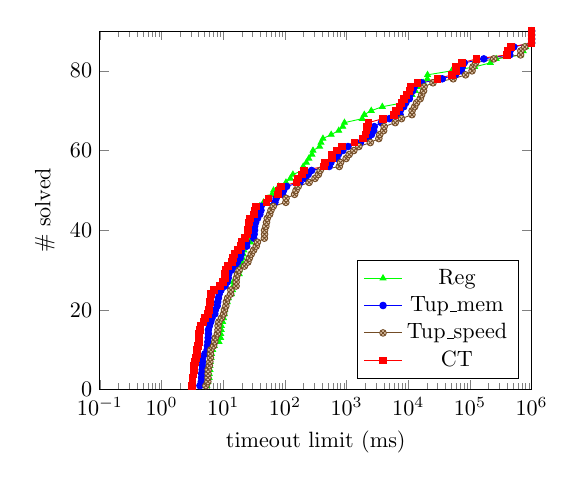
\begin{tikzpicture}[scale=0.8]
      \begin{axis}[
    xmode=log,
    ymin=0,ymax=90,
    xmin=0.1, xmax=1000000,
    every axis plot/.style={thin},
    xlabel={timeout limit (ms)},
    ylabel={\# solved},
    legend pos=south east
    % table/create on use/cumulative distribution/.style={
    %   create col/expr={\pgfmathaccuma + \thisrow{f(x)}}   
    % }
    ]
    \addplot 
    [mark=triangle*,
    mark size=1.5,
    mark options={solid},
    green] 
    coordinates {(5.389, 1)
(5.638, 2)
(5.908, 3)
(5.926, 4)
(6.086, 5)
(6.087, 6)
(6.166, 7)
(6.364, 8)
(6.469, 9)
(6.740, 10)
(7.148, 11)
(8.536, 12)
(9.080, 13)
(9.107, 14)
(9.303, 15)
(9.342, 16)
(9.805, 17)
(10.076, 18)
(10.428, 19)
(10.604, 20)
(10.907, 21)
(11.627, 22)
(12.123, 23)
(13.601, 24)
(14.151, 25)
(14.458, 26)
(14.490, 27)
(16.359, 28)
(18.190, 29)
(18.223, 30)
(18.413, 31)
(20.180, 32)
(20.506, 33)
(21.122, 34)
(21.643, 35)
(21.810, 36)
(27.563, 37)
(28.053, 38)
(28.274, 39)
(28.976, 40)
(30.018, 41)
(32.583, 42)
(32.814, 43)
(34.369, 44)
(38.523, 45)
(39.007, 46)
(44.977, 47)
(53.309, 48)
(61.875, 49)
(65.395, 50)
(79.428, 51)
(103.937, 52)
(122.565, 53)
(134.772, 54)
(193.149, 55)
(198.243, 56)
(223.375, 57)
(244.449, 58)
(274.390, 59)
(285.380, 60)
(365.560, 61)
(384.623, 62)
(413.842, 63)
(562.607, 64)
(746.251, 65)
(868.276, 66)
(924.223, 67)
(1793.623, 68)
(1937.966, 69)
(2509.726, 70)
(3797.584, 71)
(8373.485, 72)
(9593.391, 73)
(11531.366, 74)
(13031.885, 75)
(13941.016, 76)
(17694.770, 77)
(20392.242, 78)
(20545.405, 79)
(50620.318, 80)
(119540.736, 81)
(214612.883, 82)
(266484.425, 83)
(663627.605, 84)
(728667.872, 85)
(801665.108, 86)
(1000000.234, 87)
(1000000.344, 88)
(1000000.486, 89)
(1000000.515, 90)};

    \addplot 
    [blue,
    mark=*,
    mark size=1.5,
    mark options={solid}]
    coordinates {(4.188, 1)
(4.403, 2)
(4.451, 3)
(4.455, 4)
(4.562, 5)
(4.588, 6)
(4.619, 7)
(4.632, 8)
(5.046, 9)
(5.488, 10)
(5.538, 11)
(5.633, 12)
(5.705, 13)
(5.751, 14)
(5.756, 15)
(5.975, 16)
(6.278, 17)
(6.572, 18)
(7.295, 19)
(7.462, 20)
(7.979, 21)
(8.133, 22)
(8.358, 23)
(8.600, 24)
(9.209, 25)
(10.692, 26)
(11.548, 27)
(12.039, 28)
(12.248, 29)
(13.672, 30)
(15.880, 31)
(17.016, 32)
(18.711, 33)
(19.469, 34)
(19.729, 35)
(24.033, 36)
(24.051, 37)
(31.205, 38)
(31.687, 39)
(32.193, 40)
(32.329, 41)
(33.569, 42)
(35.982, 43)
(39.229, 44)
(40.895, 45)
(41.002, 46)
(68.982, 47)
(72.077, 48)
(91.486, 49)
(95.198, 50)
(106.573, 51)
(175.861, 52)
(214.260, 53)
(238.677, 54)
(271.193, 55)
(521.556, 56)
(557.425, 57)
(696.625, 58)
(735.011, 59)
(870.153, 60)
(1055.255, 61)
(1679.897, 62)
(2241.096, 63)
(2535.154, 64)
(2753.061, 65)
(2810.081, 66)
(3659.581, 67)
(4929.111, 68)
(7363.979, 69)
(7410.807, 70)
(8451.231, 71)
(9127.653, 72)
(10432.603, 73)
(10677.377, 74)
(11811.600, 75)
(12543.472, 76)
(16543.725, 77)
(35604.104, 78)
(58303.018, 79)
(72255.089, 80)
(75266.395, 81)
(80879.389, 82)
(167936.606, 83)
(442447.640, 84)
(447925.512, 85)
(514354.235, 86)
(1000001.142, 87)
(1000001.149, 88)
(1000001.277, 89)
(1000001.333, 90)};

    \addplot [brown!60!black,
    mark options={fill=brown!40},
    mark=otimes*,
    mark size=1.5]
    coordinates {(5.231, 1)
(5.629, 2)
(5.648, 3)
(5.663, 4)
(5.683, 5)
(5.943, 6)
(6.064, 7)
(6.179, 8)
(6.183, 9)
(6.295, 10)
(6.973, 11)
(7.284, 12)
(7.442, 13)
(8.037, 14)
(8.223, 15)
(8.238, 16)
(8.503, 17)
(9.384, 18)
(10.150, 19)
(10.464, 20)
(11.030, 21)
(11.224, 22)
(11.768, 23)
(13.192, 24)
(13.291, 25)
(16.148, 26)
(16.203, 27)
(16.372, 28)
(17.047, 29)
(18.087, 30)
(22.065, 31)
(25.084, 32)
(26.518, 33)
(28.470, 34)
(31.075, 35)
(34.278, 36)
(35.789, 37)
(46.424, 38)
(46.741, 39)
(46.749, 40)
(49.131, 41)
(50.337, 42)
(51.769, 43)
(56.622, 44)
(59.385, 45)
(64.673, 46)
(103.471, 47)
(104.380, 48)
(143.379, 49)
(151.391, 50)
(164.336, 51)
(246.920, 52)
(307.962, 53)
(349.129, 54)
(373.194, 55)
(761.064, 56)
(798.540, 57)
(984.391, 58)
(1100.413, 59)
(1311.163, 60)
(1581.664, 61)
(2426.014, 62)
(3330.803, 63)
(3451.164, 64)
(3985.165, 65)
(4060.894, 66)
(6149.120, 67)
(7773.303, 68)
(11478.659, 69)
(11534.975, 70)
(12707.939, 71)
(13658.601, 72)
(15631.173, 73)
(16480.122, 74)
(17709.931, 75)
(18042.131, 76)
(25195.852, 77)
(53588.555, 78)
(85036.871, 79)
(108170.261, 80)
(111741.798, 81)
(123479.329, 82)
(242924.139, 83)
(662412.696, 84)
(668282.082, 85)
(773006.352, 86)
(1000000.222, 87)
(1000000.350, 88)
(1000000.409, 89)
(1000001.208, 90)};

    \addplot 
    [red,
    mark size=1.5,
    mark=square*]
    coordinates {(3.077, 1)
(3.159, 2)
(3.165, 3)
(3.290, 4)
(3.360, 5)
(3.387, 6)
(3.499, 7)
(3.591, 8)
(3.773, 9)
(3.788, 10)
(3.878, 11)
(3.996, 12)
(3.998, 13)
(4.030, 14)
(4.235, 15)
(4.270, 16)
(4.806, 17)
(4.996, 18)
(5.677, 19)
(5.849, 20)
(5.952, 21)
(6.121, 22)
(6.164, 23)
(6.365, 24)
(7.079, 25)
(8.883, 26)
(9.951, 27)
(10.577, 28)
(10.722, 29)
(10.853, 30)
(11.910, 31)
(13.844, 32)
(14.533, 33)
(15.242, 34)
(17.301, 35)
(19.220, 36)
(19.624, 37)
(22.571, 38)
(24.789, 39)
(24.978, 40)
(25.692, 41)
(25.836, 42)
(27.326, 43)
(31.105, 44)
(32.150, 45)
(33.871, 46)
(50.022, 47)
(53.705, 48)
(77.777, 49)
(78.665, 50)
(86.000, 51)
(153.424, 52)
(163.326, 53)
(186.857, 54)
(205.347, 55)
(431.945, 56)
(447.896, 57)
(579.321, 58)
(582.538, 59)
(697.105, 60)
(845.847, 61)
(1342.019, 62)
(1841.060, 63)
(2032.310, 64)
(2086.544, 65)
(2136.864, 66)
(2259.967, 67)
(3859.192, 68)
(5928.297, 69)
(6294.023, 70)
(7189.658, 71)
(7718.920, 72)
(8552.721, 73)
(9394.659, 74)
(10400.047, 75)
(10914.835, 76)
(14065.923, 77)
(29727.731, 78)
(50913.845, 79)
(58766.196, 80)
(59010.473, 81)
(73352.608, 82)
(127355.852, 83)
(398786.693, 84)
(405416.242, 85)
(466149.784, 86)
(1000000.184, 87)
(1000000.216, 88)
(1000000.280, 89)
(1000000.721, 90)};
    \legend{Reg,Tup\_mem,Tup\_speed,CT}
  \end{axis}

    \end{tikzpicture}
    \vfill
    \caption{\textbf{Geom}. The 100 instances of this benchmark
    contain binary constraints. The variable domains are
    1..20.}
    \vspace{\baselineskip}
  \end{minipage}\qquad

\end{figure}

\newpage

\begin{figure}
  \begin{minipage}[b][10cm][s]{0.45\textwidth}
    \centering
    \vfill
    \begin{tikzpicture}[scale=0.8]
      \begin{axis}[
    xmode=log,
    ymin=0,ymax=13,
    xmin=0.1, xmax=1000000,
    every axis plot/.style={thin},
    xlabel={timeout limit (ms)},
    ylabel={\# solved},
    legend pos=south east
    % table/create on use/cumulative distribution/.style={
    %   create col/expr={\pgfmathaccuma + \thisrow{f(x)}}   
    % }
    ]
    \addplot 
    [mark=triangle*,
    mark size=1.5,
    mark options={solid},
    green] 
    coordinates {(25692.763, 1)
(52566.138, 2)
(108946.436, 3)
(221877.475, 4)
(464154.393, 5)
(959255.963, 6)
(1000000.112, 7)
(1000000.119, 8)
(1000000.125, 9)
(1000000.129, 10)
(1000000.202, 11)
(1000000.206, 12)
(1000000.220, 13)};

    \addplot 
    [blue,
    mark=*,
    mark size=1.5,
    mark options={solid}]
    coordinates {(24930.451, 1)
(51072.293, 2)
(104903.803, 3)
(218612.431, 4)
(452788.242, 5)
(938091.619, 6)
(1000000.148, 7)
(1000000.149, 8)
(1000000.179, 9)
(1000000.201, 10)
(1000000.213, 11)
(1000000.232, 12)
(1000000.236, 13)};

    \addplot [brown!60!black,
    mark options={fill=brown!40},
    mark=otimes*,
    mark size=1.5]
    table {(32168.167, 1)
(67198.233, 2)
(137576.561, 3)
(283937.740, 4)
(592360.368, 5)
(1000000.108, 6)
(1000000.110, 7)
(1000000.115, 8)
(1000000.116, 9)
(1000000.125, 10)
(1000000.180, 11)
(1000000.190, 12)
(1000000.202, 13)};

    \addplot 
    [red,
    mark size=1.5,
    mark=square*]
    table {(21084.624, 1)
(42987.264, 2)
(88183.028, 3)
(183554.060, 4)
(374851.071, 5)
(785860.510, 6)
(1000000.112, 7)
(1000000.115, 8)
(1000000.120, 9)
(1000000.183, 10)
(1000000.200, 11)
(1000000.202, 12)
(1061960.067, 13)};
    \legend{Reg,Tup\_mem,Tup\_speed,CT}
  \end{axis}

    \end{tikzpicture}
    \vfill
    \caption{\textbf{Dubois}. The 12 instances of this benchmark
      contain two constraints each, of arity 3.
      All variables are 0/1.}
    \vspace{\baselineskip}
  \end{minipage}\qquad

\end{figure}

\newpage

\begin{figure}
  \begin{minipage}[b][10cm][s]{0.45\textwidth}
    \centering
    \vfill
    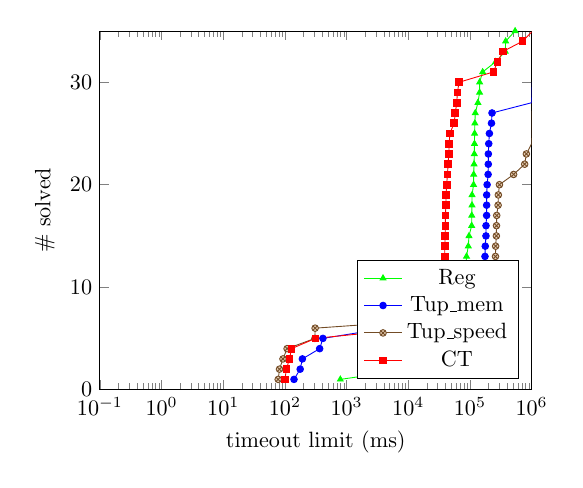
\begin{tikzpicture}[scale=0.8]
      \begin{axis}[
    xmode=log,
    ymin=0,ymax=35,
    xmin=0.1, xmax=1000000,
    every axis plot/.style={thin},
    xlabel={timeout limit (ms)},
    ylabel={\# solved},
    legend pos=south east
    % table/create on use/cumulative distribution/.style={
    %   create col/expr={\pgfmathaccuma + \thisrow{f(x)}}   
    % }
    ]
    \addplot 
    [mark=triangle*,
    mark size=1.5,
    mark options={solid},
    green] 
    coordinates {(791.560, 1)
(11472.600, 2)
(14766.696, 3)
(15745.163, 4)
(26862.099, 5)
(31778.084, 6)
(72448.015, 7)
(80752.168, 8)
(82923.009, 9)
(83683.963, 10)
(84465.445, 11)
(85764.561, 12)
(88032.555, 13)
(94011.079, 14)
(96560.156, 15)
(106648.859, 16)
(107056.591, 17)
(107933.416, 18)
(108210.305, 19)
(114497.218, 20)
(114966.358, 21)
(116658.706, 22)
(117735.741, 23)
(118508.245, 24)
(119006.430, 25)
(120178.594, 26)
(122120.270, 27)
(134711.654, 28)
(143405.319, 29)
(143582.718, 30)
(160788.320, 31)
(261709.502, 32)
(374501.791, 33)
(379347.315, 34)
(540015.740, 35)};

    \addplot 
    [blue,
    mark=*,
    mark size=1.5,
    mark options={solid}]
    coordinates {(140.425, 1)
(176.917, 2)
(192.112, 3)
(365.981, 4)
(413.133, 5)
(4403.296, 6)
(39876.347, 7)
(92306.099, 8)
(167189.458, 9)
(169366.958, 10)
(170556.481, 11)
(173851.037, 12)
(175430.330, 13)
(177265.457, 14)
(181905.169, 15)
(182312.517, 16)
(186399.578, 17)
(186652.401, 18)
(186832.299, 19)
(189971.439, 20)
(197152.408, 21)
(198415.969, 22)
(198894.284, 23)
(201831.845, 24)
(206792.806, 25)
(223634.515, 26)
(228125.105, 27)
(1001453.819, 28)
(1004586.749, 29)
(1020114.517, 30)
(1167495.643, 31)
(1316010.414, 32)
(1399844.041, 33)
(1422830.720, 34)
(1553624.496, 35)};

    \addplot [brown!60!black,
    mark options={fill=brown!40},
    mark=otimes*,
    mark size=1.5]
    coordinates {(77.848, 1)
(81.738, 2)
(93.013, 3)
(108.475, 4)
(306.721, 5)
(309.048, 6)
(71781.939, 7)
(119555.503, 8)
(232959.976, 9)
(235395.918, 10)
(237247.816, 11)
(247450.645, 12)
(259525.670, 13)
(261038.714, 14)
(268346.434, 15)
(269506.659, 16)
(271797.636, 17)
(286253.613, 18)
(288902.149, 19)
(300957.270, 20)
(510582.087, 21)
(771478.727, 22)
(822435.981, 23)
(1000367.652, 24)
(1005161.590, 25)
(1010019.345, 26)
(1010418.164, 27)
(1022093.039, 28)
(1029891.832, 29)
(1031150.393, 30)
(1034813.269, 31)
(1054519.771, 32)
(1073321.307, 33)
(1142503.375, 34)
(1301096.751, 35)};

    \addplot 
    [red,
    mark size=1.5,
    mark=square*]
    coordinates {(100.268, 1)
(105.476, 2)
(118.901, 3)
(127.592, 4)
(313.306, 5)
(13094.233, 6)
(19436.829, 7)
(34008.560, 8)
(35649.282, 9)
(36572.672, 10)
(36586.778, 11)
(38788.690, 12)
(39051.053, 13)
(39170.191, 14)
(39702.088, 15)
(39815.587, 16)
(40011.946, 17)
(40780.574, 18)
(40946.927, 19)
(41904.986, 20)
(43203.913, 21)
(44258.721, 22)
(45394.073, 23)
(46118.992, 24)
(47174.176, 25)
(55599.614, 26)
(57777.455, 27)
(61166.183, 28)
(62548.310, 29)
(66755.839, 30)
(239564.852, 31)
(281010.056, 32)
(343727.677, 33)
(713034.541, 34)
(1040781.786, 35)};
    \legend{Reg,Tup\_mem,Tup\_speed,CT}
  \end{axis}

    \end{tikzpicture}
    \vfill
    \caption{\textbf{BDD Large}.
      The 35 instances of this benchmark contain constraints
      of arity 15. The variables are 0/1.}
    \vspace{\baselineskip}
  \end{minipage}\qquad
\end{figure}


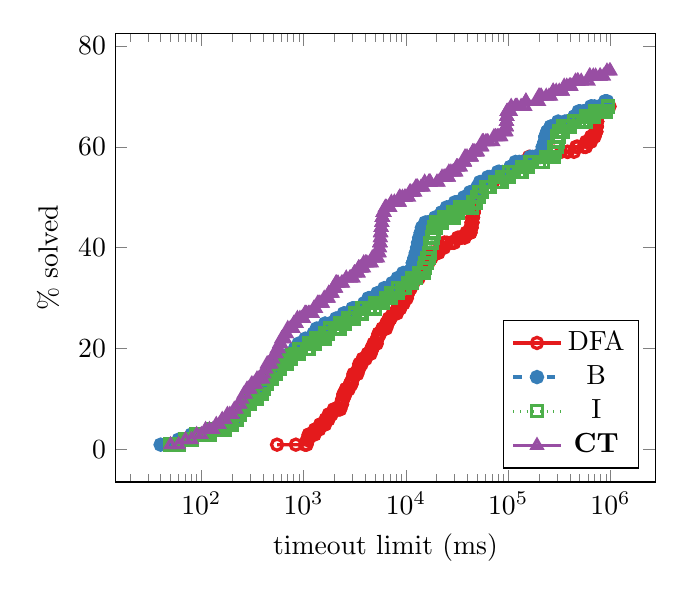
\begin{tikzpicture}%[scale=0.9]
  \begin{axis}[
    xmode=log,
    every axis plot/.style={thin},
    xlabel={timeout limit (ms)},
    ylabel={\% solved},
    legend pos=south east,
    cycle list/Set1-6,
            % define fill color for the marker
            mark list fill={.!75!white},
            mark options={solid},
            cycle multiindex* list={
                Set1-6
                    \nextlist
                [3 of]linestyles
                    \nextlist
                very thick
                \nextlist
                mark=o,
                mark=*,
                mark=square,
                mark=triangle,
                mark=+
            },
    ]

    \addplot
    coordinates {
      (550, 1)
      (840, 1)
      (1030, 1)
      (1070, 1)
      (1080, 2)
      (1090, 2)
      (1100, 2)
      (1110, 2)
      (1120, 3)
      (1130, 3)
      (1140, 3)
      (1170, 3)
      (1180, 3)
      (1190, 3)
      (1280, 3)
      (1290, 4)
      (1300, 4)
      (1340, 4)
      (1360, 4)
      (1420, 4)
      (1450, 5)
      (1460, 5)
      (1550, 5)
      (1590, 5)
      (1610, 5)
      (1620, 5)
      (1640, 6)
      (1650, 6)
      (1680, 6)
      (1740, 6)
      (1750, 6)
      (1760, 7)
      (1780, 7)
      (1810, 7)
      (1830, 7)
      (1880, 7)
      (1970, 8)
      (2010, 8)
      (2070, 8)
      (2160, 8)
      (2180, 8)
      (2240, 8)
      (2280, 8)
      (2300, 9)
      (2320, 9)
      (2340, 9)
      (2360, 9)
      (2370, 9)
      (2380, 10)
      (2400, 10)
      (2420, 10)
      (2430, 10)
      (2440, 10)
      (2450, 11)
      (2460, 11)
      (2480, 11)
      (2490, 11)
      (2550, 11)
      (2560, 11)
      (2590, 12)
      (2600, 12)
      (2620, 12)
      (2630, 12)
      (2750, 12)
      (2760, 12)
      (2830, 13)
      (2840, 13)
      (2880, 13)
      (2910, 13)
      (2930, 13)
      (2940, 13)
      (2990, 14)
      (3000, 14)
      (3010, 14)
      (3030, 14)
      (3070, 15)
      (3160, 15)
      (3190, 15)
      (3250, 15)
      (3260, 15)
      (3290, 15)
      (3350, 15)
      (3400, 16)
      (3430, 16)
      (3450, 16)
      (3480, 16)
      (3500, 17)
      (3550, 17)
      (3630, 17)
      (3650, 17)
      (3700, 17)
      (3780, 18)
      (3830, 18)
      (3870, 18)
      (3950, 18)
      (3960, 18)
      (4050, 18)
      (4220, 19)
      (4320, 19)
      (4340, 19)
      (4350, 19)
      (4520, 19)
      (4590, 20)
      (4600, 20)
      (4640, 20)
      (4670, 20)
      (4680, 20)
      (4710, 20)
      (4820, 21)
      (4870, 21)
      (4940, 21)
      (4950, 21)
      (4980, 21)
      (5180, 21)
      (5210, 22)
      (5220, 22)
      (5240, 22)
      (5260, 22)
      (5270, 22)
      (5280, 22)
      (5400, 23)
      (5430, 23)
      (5480, 23)
      (5520, 23)
      (5590, 23)
      (5880, 24)
      (5930, 24)
      (5970, 24)
      (6170, 24)
      (6280, 24)
      (6400, 24)
      (6420, 25)
      (6460, 25)
      (6530, 25)
      (6620, 25)
      (6630, 25)
      (6650, 25)
      (6800, 26)
      (6960, 26)
      (7020, 26)
      (7040, 26)
      (7090, 26)
      (7430, 27)
      (7750, 27)
      (7760, 27)
      (7790, 27)
      (7880, 27)
      (8170, 27)
      (8240, 28)
      (8300, 28)
      (8310, 28)
      (8610, 28)
      (8770, 28)
      (8800, 28)
      (8950, 29)
      (9050, 29)
      (9240, 29)
      (9270, 29)
      (9380, 29)
      (9410, 29)
      (9500, 29)
      (9580, 30)
      (9650, 30)
      (9840, 30)
      (9950, 30)
      (10200, 30)
      (10380, 31)
      (10400, 31)
      (10410, 31)
      (10450, 31)
      (10460, 31)
      (10490, 31)
      (10540, 32)
      (10760, 32)
      (10890, 32)
      (10970, 32)
      (11060, 32)
      (11170, 32)
      (11200, 33)
      (11440, 33)
      (11550, 33)
      (11610, 33)
      (11620, 33)
      (11820, 33)
      (11860, 34)
      (12230, 34)
      (12550, 34)
      (12670, 34)
      (12770, 34)
      (13100, 34)
      (13360, 34)
      (13500, 35)
      (13640, 35)
      (13740, 35)
      (13820, 35)
      (14310, 35)
      (14320, 35)
      (14490, 36)
      (14650, 36)
      (14920, 36)
      (14940, 36)
      (15080, 36)
      (15140, 36)
      (15490, 36)
      (15660, 37)
      (15680, 37)
      (16050, 37)
      (16070, 37)
      (16230, 37)
      (16600, 37)
      (16730, 38)
      (17030, 38)
      (17090, 38)
      (17400, 38)
      (17510, 38)
      (17800, 38)
      (17990, 39)
      (18580, 39)
      (18870, 39)
      (19950, 39)
      (19980, 39)
      (20460, 39)
      (20820, 39)
      (21550, 40)
      (21800, 40)
      (21960, 40)
      (22580, 40)
      (22650, 40)
      (23570, 40)
      (23810, 41)
      (23840, 41)
      (25170, 41)
      (27570, 41)
      (28160, 41)
      (29400, 41)
      (29590, 41)
      (32170, 42)
      (33320, 42)
      (34310, 42)
      (34450, 42)
      (35060, 42)
      (37590, 42)
      (39070, 43)
      (41030, 43)
      (42030, 43)
      (42110, 43)
      (42560, 43)
      (42590, 43)
      (42690, 43)
      (42720, 44)
      (43170, 44)
      (43570, 44)
      (43610, 44)
      (43620, 44)
      (43860, 44)
      (43880, 45)
      (43970, 45)
      (44060, 45)
      (44510, 45)
      (44590, 45)
      (44620, 45)
      (44670, 46)
      (44690, 46)
      (44850, 46)
      (45080, 46)
      (45130, 46)
      (45140, 46)
      (45650, 47)
      (45720, 47)
      (45810, 47)
      (45840, 47)
      (45870, 47)
      (45910, 47)
      (46000, 48)
      (46230, 48)
      (46310, 48)
      (46580, 48)
      (46600, 48)
      (46640, 48)
      (46680, 48)
      (46730, 49)
      (46880, 49)
      (47010, 49)
      (47040, 49)
      (47130, 49)
      (47520, 49)
      (47760, 50)
      (47990, 50)
      (48040, 50)
      (48180, 50)
      (48400, 50)
      (48420, 50)
      (48490, 50)
      (48500, 51)
      (48510, 51)
      (48630, 51)
      (48710, 51)
      (48880, 51)
      (49120, 51)
      (51040, 52)
      (52050, 52)
      (53070, 52)
      (53920, 52)
      (54160, 52)
      (55650, 52)
      (57610, 53)
      (62030, 53)
      (67210, 53)
      (68040, 53)
      (69500, 53)
      (70070, 53)
      (71260, 53)
      (75510, 54)
      (79160, 54)
      (79890, 54)
      (86410, 54)
      (90560, 54)
      (93850, 54)
      (93910, 55)
      (94840, 55)
      (98270, 55)
      (98610, 55)
      (99880, 55)
      (101600, 55)
      (106800, 55)
      (107940, 56)
      (113230, 56)
      (118040, 56)
      (123230, 56)
      (125250, 56)
      (126460, 56)
      (136850, 57)
      (141410, 57)
      (145590, 57)
      (146260, 57)
      (147100, 57)
      (156470, 57)
      (159560, 58)
      (163380, 58)
      (183150, 58)
      (188630, 58)
      (203020, 58)
      (221140, 58)
      (252130, 58)
      (280600, 59)
      (281920, 59)
      (329390, 59)
      (378010, 59)
      (382430, 59)
      (439630, 59)
      (461470, 60)
      (471890, 60)
      (480190, 60)
      (547470, 60)
      (565750, 60)
      (567980, 60)
      (576020, 60)
      (577420, 61)
      (603180, 61)
      (615930, 61)
      (625640, 61)
      (640580, 61)
      (642660, 61)
      (645690, 62)
      (649280, 62)
      (652550, 62)
      (667400, 62)
      (678420, 62)
      (690100, 62)
      (698600, 62)
      (708040, 63)
      (720000, 63)
      (720800, 63)
      (722220, 63)
      (724200, 63)
      (724530, 63)
      (728770, 64)
      (730570, 64)
      (730590, 64)
      (731370, 64)
      (732210, 64)
      (733600, 64)
      (733910, 65)
      (734530, 65)
      (735560, 65)
      (735840, 65)
      (737480, 65)
      (737920, 65)
      (738690, 65)
      (739660, 66)
      (739730, 66)
      (740600, 66)
      (743400, 66)
      (744510, 66)
      (745370, 66)
      (745640, 67)
      (751150, 67)
      (751910, 67)
      (752040, 67)
      (790090, 67)
      (828510, 67)
      (869340, 67)
      (921350, 68)
      (925960, 68)
      (939670, 68)
      (978230, 68)
      
    };
    \addplot
    coordinates {
      (40, 1)
      (50, 1)
      (60, 2)
      (70, 2)
      (80, 3)
      (90, 3)
      (100, 3)
      (120, 4)
      (130, 4)
      (140, 4)
      (160, 5)
      (170, 5)
      (180, 5)
      (190, 6)
      (200, 6)
      (210, 6)
      (220, 7)
      (230, 7)
      (240, 7)
      (250, 8)
      (260, 8)
      (270, 9)
      (290, 9)
      (300, 10)
      (310, 10)
      (320, 10)
      (330, 10)
      (340, 11)
      (350, 11)
      (360, 11)
      (370, 12)
      (380, 12)
      (390, 12)
      (400, 12)
      (410, 13)
      (420, 13)
      (430, 14)
      (440, 14)
      (450, 14)
      (470, 14)
      (500, 15)
      (510, 15)
      (520, 15)
      (530, 15)
      (540, 16)
      (550, 16)
      (560, 16)
      (570, 17)
      (580, 17)
      (590, 17)
      (610, 17)
      (620, 17)
      (630, 17)
      (640, 18)
      (650, 18)
      (670, 18)
      (690, 18)
      (720, 18)
      (730, 19)
      (780, 19)
      (790, 19)
      (810, 19)
      (820, 20)
      (830, 20)
      (840, 20)
      (850, 20)
      (860, 20)
      (890, 21)
      (920, 21)
      (930, 21)
      (1000, 21)
      (1030, 21)
      (1040, 22)
      (1140, 22)
      (1150, 22)
      (1210, 22)
      (1230, 22)
      (1240, 22)
      (1250, 23)
      (1260, 23)
      (1310, 23)
      (1330, 23)
      (1340, 24)
      (1420, 24)
      (1550, 24)
      (1560, 24)
      (1570, 24)
      (1600, 24)
      (1610, 24)
      (1620, 25)
      (1800, 25)
      (1890, 25)
      (1970, 25)
      (1980, 25)
      (2010, 25)
      (2080, 26)
      (2210, 26)
      (2220, 26)
      (2230, 26)
      (2410, 26)
      (2440, 26)
      (2470, 27)
      (2510, 27)
      (2670, 27)
      (2760, 27)
      (2790, 27)
      (2810, 27)
      (2950, 27)
      (3000, 28)
      (3070, 28)
      (3110, 28)
      (3720, 28)
      (3850, 28)
      (3900, 28)
      (3910, 29)
      (3940, 29)
      (3960, 29)
      (4020, 29)
      (4070, 29)
      (4080, 29)
      (4200, 29)
      (4300, 30)
      (4380, 30)
      (4430, 30)
      (4970, 30)
      (4990, 30)
      (5250, 31)
      (5330, 31)
      (5380, 31)
      (5390, 31)
      (5490, 31)
      (5690, 31)
      (6140, 32)
      (6640, 32)
      (6980, 32)
      (7080, 32)
      (7300, 32)
      (7350, 33)
      (7450, 33)
      (7810, 33)
      (7820, 33)
      (8070, 33)
      (8160, 33)
      (8290, 34)
      (8620, 34)
      (8650, 34)
      (8710, 34)
      (8890, 34)
      (9100, 34)
      (9200, 34)
      (9390, 35)
      (9880, 35)
      (9950, 35)
      (11150, 35)
      (11330, 35)
      (11440, 35)
      (11450, 36)
      (11490, 36)
      (11520, 36)
      (11560, 36)
      (11570, 36)
      (11610, 36)
      (11710, 36)
      (11720, 37)
      (11730, 37)
      (11740, 37)
      (11800, 37)
      (11840, 37)
      (12090, 37)
      (12110, 38)
      (12200, 38)
      (12390, 38)
      (12460, 38)
      (12490, 38)
      (12510, 39)
      (12550, 39)
      (12660, 39)
      (12750, 39)
      (12770, 39)
      (12850, 39)
      (12890, 40)
      (12910, 40)
      (13000, 40)
      (13010, 40)
      (13020, 40)
      (13180, 41)
      (13190, 41)
      (13330, 41)
      (13380, 41)
      (13400, 41)
      (13490, 42)
      (13650, 42)
      (13710, 42)
      (13720, 42)
      (13880, 42)
      (14000, 43)
      (14020, 43)
      (14060, 43)
      (14070, 43)
      (14180, 43)
      (14190, 43)
      (14250, 43)
      (14330, 44)
      (14640, 44)
      (14810, 44)
      (15030, 44)
      (15280, 44)
      (15330, 44)
      (15450, 45)
      (16080, 45)
      (16490, 45)
      (16840, 45)
      (17230, 45)
      (17370, 45)
      (19310, 46)
      (19860, 46)
      (20520, 46)
      (20670, 46)
      (20950, 46)
      (21010, 46)
      (21410, 46)
      (22390, 47)
      (22400, 47)
      (23060, 47)
      (23670, 47)
      (23770, 47)
      (23990, 47)
      (25040, 48)
      (26030, 48)
      (27860, 48)
      (28430, 48)
      (29420, 48)
      (29430, 48)
      (29770, 48)
      (30130, 49)
      (31300, 49)
      (31470, 49)
      (32360, 49)
      (36130, 49)
      (36670, 49)
      (36960, 50)
      (37610, 50)
      (39020, 50)
      (39870, 50)
      (40280, 50)
      (41080, 50)
      (42090, 50)
      (42340, 51)
      (42730, 51)
      (44460, 51)
      (46790, 51)
      (47300, 51)
      (48720, 51)
      (49900, 52)
      (50190, 52)
      (50380, 52)
      (51560, 52)
      (51670, 52)
      (52930, 52)
      (53070, 53)
      (53180, 53)
      (55820, 53)
      (57090, 53)
      (57910, 53)
      (61660, 53)
      (62930, 53)
      (63380, 54)
      (65710, 54)
      (70600, 54)
      (70870, 54)
      (72970, 54)
      (77350, 54)
      (79280, 55)
      (79890, 55)
      (81410, 55)
      (81770, 55)
      (81780, 55)
      (87640, 55)
      (101330, 55)
      (105170, 56)
      (105410, 56)
      (105640, 56)
      (109260, 56)
      (115720, 56)
      (117110, 56)
      (117810, 57)
      (128530, 57)
      (140070, 57)
      (144570, 57)
      (145440, 57)
      (146750, 57)
      (164060, 58)
      (173000, 58)
      (183390, 58)
      (189860, 58)
      (203540, 58)
      (204830, 58)
      (207670, 58)
      (212230, 59)
      (214190, 59)
      (214370, 59)
      (215170, 59)
      (215850, 59)
      (216790, 59)
      (217510, 60)
      (218870, 60)
      (219890, 60)
      (223170, 60)
      (224760, 60)
      (225170, 60)
      (225860, 60)
      (226850, 61)
      (227440, 61)
      (228660, 61)
      (229240, 61)
      (230000, 61)
      (231220, 62)
      (231360, 62)
      (231560, 62)
      (231610, 62)
      (232280, 62)
      (235010, 62)
      (235380, 62)
      (240580, 63)
      (241080, 63)
      (241120, 63)
      (247070, 63)
      (253910, 63)
      (259150, 63)
      (259930, 64)
      (260450, 64)
      (269680, 64)
      (290930, 64)
      (293180, 64)
      (301170, 64)
      (307460, 65)
      (358130, 65)
      (373680, 65)
      (395010, 65)
      (400330, 65)
      (415600, 65)
      (417390, 65)
      (444260, 66)
      (445130, 66)
      (449310, 66)
      (474370, 66)
      (482150, 66)
      (482210, 66)
      (487090, 67)
      (500040, 67)
      (502640, 67)
      (542500, 67)
      (550590, 67)
      (553150, 67)
      (566020, 67)
      (645270, 68)
      (653190, 68)
      (697470, 68)
      (777770, 68)
      (794860, 68)
      (879060, 68)
      (886150, 69)
      (896370, 69)
      (901390, 69)
      (901730, 69)
      (925510, 69)
      
    };
    \addplot
    coordinates {
      (50, 1)
      (60, 1)
      (70, 2)
      (80, 2)
      (90, 3)
      (100, 3)
      (110, 3)
      (120, 3)
      (130, 4)
      (140, 4)
      (150, 4)
      (160, 4)
      (170, 4)
      (180, 5)
      (190, 5)
      (200, 5)
      (220, 6)
      (230, 7)
      (240, 7)
      (250, 8)
      (260, 8)
      (270, 9)
      (280, 9)
      (290, 9)
      (300, 9)
      (310, 10)
      (320, 10)
      (340, 10)
      (350, 10)
      (360, 11)
      (380, 11)
      (390, 11)
      (400, 12)
      (410, 12)
      (420, 13)
      (430, 13)
      (440, 13)
      (450, 14)
      (460, 14)
      (470, 14)
      (490, 14)
      (500, 15)
      (520, 15)
      (530, 15)
      (540, 16)
      (550, 16)
      (560, 16)
      (570, 16)
      (580, 16)
      (600, 17)
      (630, 17)
      (650, 17)
      (660, 17)
      (690, 17)
      (720, 18)
      (730, 18)
      (750, 18)
      (770, 19)
      (820, 19)
      (860, 19)
      (870, 19)
      (890, 19)
      (900, 20)
      (910, 20)
      (930, 20)
      (940, 20)
      (1090, 20)
      (1120, 20)
      (1130, 21)
      (1150, 21)
      (1170, 21)
      (1180, 21)
      (1280, 21)
      (1290, 21)
      (1330, 22)
      (1400, 22)
      (1500, 22)
      (1550, 22)
      (1560, 22)
      (1610, 22)
      (1620, 23)
      (1630, 23)
      (1700, 23)
      (1720, 23)
      (1730, 23)
      (1810, 24)
      (2050, 24)
      (2150, 24)
      (2180, 24)
      (2190, 24)
      (2220, 24)
      (2250, 24)
      (2270, 25)
      (2290, 25)
      (2320, 25)
      (2470, 25)
      (2540, 25)
      (2700, 26)
      (2740, 26)
      (2880, 26)
      (2910, 26)
      (3080, 26)
      (3120, 26)
      (3200, 27)
      (3550, 27)
      (3580, 27)
      (3660, 27)
      (3680, 27)
      (3700, 27)
      (3770, 28)
      (3870, 28)
      (4370, 28)
      (4390, 28)
      (4460, 28)
      (5010, 28)
      (5060, 29)
      (5190, 29)
      (5330, 29)
      (5410, 29)
      (5510, 29)
      (5710, 29)
      (5980, 29)
      (6470, 30)
      (6700, 30)
      (6780, 30)
      (6810, 30)
      (6980, 30)
      (7070, 30)
      (7220, 31)
      (7650, 31)
      (7850, 31)
      (7950, 31)
      (7980, 31)
      (8140, 31)
      (8240, 31)
      (8400, 32)
      (9230, 32)
      (9260, 32)
      (9320, 32)
      (9390, 32)
      (9810, 32)
      (10590, 33)
      (11030, 33)
      (11090, 33)
      (11240, 33)
      (11370, 33)
      (11400, 33)
      (11570, 34)
      (11630, 34)
      (11880, 34)
      (12210, 34)
      (12510, 34)
      (12520, 34)
      (12550, 34)
      (13520, 35)
      (14450, 35)
      (14750, 35)
      (14800, 35)
      (15040, 35)
      (15080, 36)
      (15130, 36)
      (15210, 36)
      (15370, 36)
      (15390, 36)
      (15410, 37)
      (15470, 37)
      (15620, 37)
      (15980, 37)
      (16100, 37)
      (16150, 37)
      (16190, 38)
      (16490, 38)
      (16590, 38)
      (16640, 38)
      (16680, 38)
      (16720, 38)
      (16750, 39)
      (16800, 39)
      (16870, 39)
      (16950, 39)
      (17070, 39)
      (17090, 39)
      (17100, 40)
      (17130, 40)
      (17170, 40)
      (17180, 40)
      (17190, 40)
      (17220, 40)
      (17300, 41)
      (17550, 41)
      (17730, 41)
      (17760, 41)
      (17820, 41)
      (17950, 41)
      (17980, 41)
      (18060, 42)
      (18080, 42)
      (18100, 42)
      (18150, 42)
      (18230, 42)
      (18330, 42)
      (18460, 43)
      (18480, 43)
      (18580, 43)
      (18590, 43)
      (18700, 43)
      (18840, 43)
      (18920, 43)
      (18960, 44)
      (19300, 44)
      (19410, 44)
      (19560, 44)
      (19570, 44)
      (19640, 44)
      (19760, 45)
      (19830, 45)
      (20370, 45)
      (21220, 45)
      (21880, 45)
      (22610, 45)
      (23680, 46)
      (24090, 46)
      (25400, 46)
      (25580, 46)
      (26310, 46)
      (27720, 46)
      (29250, 46)
      (29300, 47)
      (29420, 47)
      (30980, 47)
      (31300, 47)
      (31430, 47)
      (32120, 47)
      (33870, 48)
      (34700, 48)
      (36390, 48)
      (37860, 48)
      (38390, 48)
      (40430, 48)
      (44370, 48)
      (45220, 49)
      (45850, 49)
      (46730, 49)
      (47040, 49)
      (47590, 49)
      (47970, 49)
      (49360, 50)
      (49800, 50)
      (50400, 50)
      (50510, 50)
      (50780, 50)
      (51450, 50)
      (51540, 51)
      (51650, 51)
      (52320, 51)
      (53220, 51)
      (53570, 51)
      (55250, 51)
      (61360, 52)
      (61840, 52)
      (64020, 52)
      (64590, 52)
      (65270, 52)
      (65960, 52)
      (75460, 53)
      (80010, 53)
      (80590, 53)
      (80850, 53)
      (82360, 53)
      (84470, 53)
      (85710, 53)
      (88220, 54)
      (90130, 54)
      (90670, 54)
      (93840, 54)
      (95870, 54)
      (100350, 54)
      (101240, 55)
      (112490, 55)
      (113550, 55)
      (127990, 55)
      (129810, 55)
      (131940, 55)
      (137030, 55)
      (137140, 56)
      (138470, 56)
      (140790, 56)
      (147540, 56)
      (156920, 56)
      (157130, 56)
      (162560, 57)
      (162760, 57)
      (169630, 57)
      (170370, 57)
      (198730, 57)
      (219630, 57)
      (236800, 58)
      (248230, 58)
      (259520, 58)
      (265820, 58)
      (273280, 58)
      (276470, 58)
      (279690, 58)
      (280230, 59)
      (281590, 59)
      (281810, 59)
      (282220, 59)
      (282390, 59)
      (284210, 59)
      (284410, 60)
      (286450, 60)
      (288270, 60)
      (288290, 60)
      (292840, 60)
      (295540, 60)
      (296190, 60)
      (298980, 61)
      (299550, 61)
      (299870, 61)
      (300160, 61)
      (300600, 61)
      (302190, 61)
      (303070, 62)
      (303280, 62)
      (307930, 62)
      (308440, 62)
      (311430, 62)
      (312510, 62)
      (313510, 62)
      (315280, 63)
      (317550, 63)
      (322930, 63)
      (329550, 63)
      (342630, 63)
      (343570, 63)
      (346140, 64)
      (353150, 64)
      (361750, 64)
      (374030, 64)
      (382470, 64)
      (404230, 64)
      (437270, 65)
      (492850, 65)
      (494920, 65)
      (538040, 65)
      (551680, 65)
      (565550, 65)
      (577170, 65)
      (581290, 66)
      (583270, 66)
      (606290, 66)
      (649170, 66)
      (680520, 66)
      (689910, 66)
      (716250, 67)
      (770340, 67)
      (809510, 67)
      (812480, 67)
      (861730, 67)
      (862310, 67)
      (908880, 67)
      (945850, 68)
      (946540, 68)
      
    };
    \addplot
    coordinates {
      (50, 1)
      (60, 1)
      (70, 2)
      (80, 2)
      (90, 3)
      (100, 3)
      (110, 4)
      (120, 4)
      (130, 4)
      (140, 5)
      (150, 5)
      (160, 6)
      (170, 6)
      (180, 7)
      (190, 7)
      (200, 7)
      (210, 8)
      (220, 8)
      (230, 9)
      (240, 9)
      (250, 10)
      (260, 11)
      (270, 11)
      (280, 12)
      (290, 12)
      (300, 12)
      (310, 13)
      (320, 13)
      (340, 13)
      (350, 14)
      (360, 14)
      (390, 14)
      (400, 14)
      (410, 15)
      (420, 16)
      (430, 16)
      (440, 17)
      (450, 17)
      (460, 17)
      (470, 17)
      (480, 17)
      (490, 18)
      (500, 18)
      (520, 19)
      (530, 19)
      (540, 19)
      (550, 20)
      (560, 20)
      (570, 20)
      (580, 21)
      (590, 21)
      (600, 21)
      (610, 22)
      (620, 22)
      (640, 22)
      (650, 22)
      (670, 23)
      (680, 23)
      (700, 24)
      (740, 24)
      (750, 24)
      (760, 24)
      (790, 24)
      (800, 25)
      (820, 25)
      (840, 25)
      (850, 25)
      (870, 26)
      (920, 26)
      (950, 26)
      (970, 26)
      (1000, 26)
      (1030, 27)
      (1040, 27)
      (1070, 27)
      (1120, 27)
      (1150, 27)
      (1180, 27)
      (1220, 27)
      (1260, 28)
      (1270, 28)
      (1290, 28)
      (1310, 28)
      (1370, 29)
      (1410, 29)
      (1420, 29)
      (1450, 29)
      (1500, 29)
      (1520, 29)
      (1530, 29)
      (1590, 30)
      (1700, 30)
      (1710, 30)
      (1750, 30)
      (1760, 31)
      (1830, 31)
      (1840, 31)
      (1880, 31)
      (1910, 31)
      (1940, 32)
      (1950, 32)
      (1970, 32)
      (2040, 32)
      (2060, 32)
      (2070, 33)
      (2080, 33)
      (2110, 33)
      (2170, 33)
      (2350, 33)
      (2410, 33)
      (2610, 34)
      (2830, 34)
      (2860, 34)
      (2900, 34)
      (3040, 34)
      (3050, 34)
      (3130, 35)
      (3140, 35)
      (3340, 35)
      (3410, 35)
      (3420, 35)
      (3450, 36)
      (3460, 36)
      (3560, 36)
      (3610, 36)
      (3660, 36)
      (3710, 36)
      (3860, 36)
      (3870, 37)
      (4040, 37)
      (4150, 37)
      (4410, 37)
      (4610, 37)
      (4690, 38)
      (4910, 38)
      (4970, 38)
      (5020, 38)
      (5070, 38)
      (5290, 38)
      (5340, 39)
      (5350, 39)
      (5380, 39)
      (5470, 39)
      (5480, 39)
      (5490, 40)
      (5510, 40)
      (5530, 40)
      (5540, 41)
      (5550, 41)
      (5560, 41)
      (5570, 41)
      (5590, 41)
      (5610, 41)
      (5620, 42)
      (5630, 42)
      (5640, 43)
      (5650, 43)
      (5670, 43)
      (5680, 43)
      (5700, 44)
      (5710, 44)
      (5730, 44)
      (5740, 44)
      (5760, 44)
      (5780, 45)
      (5790, 45)
      (5820, 45)
      (5830, 45)
      (5840, 46)
      (5850, 46)
      (5870, 46)
      (5900, 46)
      (5910, 46)
      (5920, 46)
      (5940, 46)
      (5960, 47)
      (5970, 47)
      (5980, 47)
      (6030, 47)
      (6090, 47)
      (6150, 47)
      (6280, 48)
      (6340, 48)
      (6480, 48)
      (6840, 48)
      (6970, 48)
      (7210, 49)
      (7710, 49)
      (7730, 49)
      (8490, 49)
      (8620, 49)
      (8630, 49)
      (8660, 50)
      (8750, 50)
      (9250, 50)
      (9750, 50)
      (9790, 50)
      (9980, 50)
      (10650, 50)
      (10890, 51)
      (11070, 51)
      (11130, 51)
      (11520, 51)
      (11740, 51)
      (12240, 51)
      (12470, 52)
      (12750, 52)
      (12870, 52)
      (13000, 52)
      (14050, 52)
      (14780, 52)
      (15250, 53)
      (16740, 53)
      (17090, 53)
      (17150, 53)
      (17300, 53)
      (20090, 53)
      (20650, 53)
      (22530, 54)
      (23590, 54)
      (24080, 54)
      (24600, 54)
      (25950, 54)
      (26010, 54)
      (26310, 55)
      (27520, 55)
      (28910, 55)
      (29020, 55)
      (29830, 55)
      (30330, 55)
      (30860, 55)
      (31320, 56)
      (31440, 56)
      (31810, 56)
      (32180, 56)
      (33910, 56)
      (34120, 56)
      (36930, 57)
      (36940, 57)
      (37060, 57)
      (37240, 57)
      (37300, 57)
      (37490, 57)
      (37850, 58)
      (39550, 58)
      (42240, 58)
      (42540, 58)
      (43230, 58)
      (43500, 58)
      (43650, 58)
      (44950, 59)
      (45410, 59)
      (46610, 59)
      (48590, 59)
      (49050, 59)
      (50170, 59)
      (53630, 60)
      (54160, 60)
      (54430, 60)
      (54450, 60)
      (54490, 60)
      (54920, 60)
      (55330, 60)
      (55870, 61)
      (57260, 61)
      (60490, 61)
      (62160, 61)
      (63280, 61)
      (71010, 61)
      (72590, 62)
      (75040, 62)
      (75370, 62)
      (78200, 62)
      (80830, 62)
      (83350, 62)
      (84800, 62)
      (90460, 63)
      (92080, 63)
      (93140, 63)
      (93590, 63)
      (94730, 63)
      (94900, 63)
      (94980, 64)
      (95250, 64)
      (95500, 64)
      (95540, 64)
      (95730, 64)
      (95770, 64)
      (95780, 65)
      (95870, 65)
      (96110, 65)
      (96160, 65)
      (96170, 65)
      (96290, 65)
      (96430, 65)
      (96470, 66)
      (96520, 66)
      (96920, 66)
      (96930, 66)
      (97190, 66)
      (97330, 66)
      (97410, 67)
      (97580, 67)
      (97630, 67)
      (100660, 67)
      (102990, 67)
      (103230, 67)
      (105320, 67)
      (106900, 68)
      (117510, 68)
      (120220, 68)
      (122290, 68)
      (133710, 68)
      (145720, 68)
      (148400, 69)
      (149210, 69)
      (149390, 69)
      (188660, 69)
      (190110, 69)
      (198370, 69)
      (199080, 70)
      (203260, 70)
      (205030, 70)
      (210860, 70)
      (235310, 70)
      (250470, 70)
      (260550, 70)
      (274190, 71)
      (275860, 71)
      (294700, 71)
      (315240, 71)
      (338260, 71)
      (339770, 71)
      (352710, 72)
      (373740, 72)
      (395750, 72)
      (399990, 72)
      (407380, 72)
      (409390, 72)
      (410490, 72)
      (454610, 73)
      (474090, 73)
      (476710, 73)
      (482760, 73)
      (517330, 73)
      (606460, 73)
      (623230, 74)
      (630420, 74)
      (679300, 74)
      (716240, 74)
      (788320, 74)
      (796770, 74)
      (855630, 74)
      (923830, 75)
      (980220, 75)
      (995840, 75)
      
    };
    

    \legend{ DFA, B, I, \textbf{CT} }
  \end{axis}

\end{tikzpicture}

% \clearpage
% \section{Bugfix}

% \begin{tabular}{cc}
%   \begin{tikzpicture}[scale=0.9]
%     \begin{axis}[
    xmode=log,
    every axis plot/.style={thin},
    xlabel={timeout limit (ms)},
    ylabel={\# solved},
    legend pos=south east
    % table/create on use/cumulative distribution/.style={
    %   create col/expr={\pgfmathaccuma + \thisrow{f(x)}}   
    % }
    ]

    \addplot [brown!60!black,
    mark options={fill=brown!40},
    mark=otimes*,
    mark size=1.5]
    coordinates {
    (305.779,1) (915.082,2) (1058.048,3) (1186.900,4) (3004.507,5) (3492.884,6) (5591.157,7) (7535.071,8) (8895.567,9) (38113.365,10)
    };

    \addplot 
    [red,
    mark size=1.5,
    mark=square*]
    coordinates {
    (336.121,1) (1041.664,2) (1206.262,3) (1341.404,4) (3444.105,5) (4186.919,6) (6308.416,7) (8544.820,8) (10473.936,9) (44033.894,10)
    };

    \legend{Bugfree,Buggy}
  \end{axis}

%   \end{tikzpicture}
%   &
%   \begin{tikzpicture}[scale=0.9]
%     \begin{axis}[
    xmode=log,
    every axis plot/.style={thin},
    xlabel={timeout limit (ms)},
    ylabel={\# solved},
    legend pos=south east
    % table/create on use/cumulative distribution/.style={
    %   create col/expr={\pgfmathaccuma + \thisrow{f(x)}}   
    % }
    ]

    \addplot [brown!60!black,
    mark options={fill=brown!40},
    mark=otimes*,
    mark size=1.5]
    coordinates {
    (2684.556,1) (3037.945,2) (4338.162,3) (5771.940,4) (24541.853,5) (27967.347,6) (36060.594,7) (68735.220,8) (103641.866,9) (244658.378,10)
    };

    \addplot 
    [red,
    mark size=1.5,
    mark=square*]
    coordinates {
    (2972.726,1) (3598.228,2) (5008.444,3) (6631.690,4) (28562.240,5) (31320.804,6) (41281.695,7) (77943.893,8) (116106.950,9) (286321.319,10)
    };

    \legend{Bugfree,Buggy}
  \end{axis}

%   \end{tikzpicture}
%   \\
%   \begin{tikzpicture}[scale=0.9]
%     \begin{axis}[
    xmode=log,
    every axis plot/.style={thin},
    xlabel={timeout limit (ms)},
    ylabel={\# solved},
    legend pos=south east
    % table/create on use/cumulative distribution/.style={
    %   create col/expr={\pgfmathaccuma + \thisrow{f(x)}}   
    % }
    ]

    \addplot [brown!60!black,
    mark options={fill=brown!40},
    mark=otimes*,
    mark size=1.5]
    coordinates {
    (0.088,1) (0.158,2) (0.202,3) (0.516,4) (0.795,5) (1.920,6) (3.342,7) (3.451,8) (3.630,9) (4.296,10) (8.532,11) (15.844,12) (27.743,13) (552.500,14) (3492.300,15) (300000.326,16) (300000.545,17) (300000.626,18) (300000.719,19) (300000.984,20)
    };

    \addplot 
    [red,
    mark size=1.5,
    mark=square*]
    coordinates {
    (0.095,1) (0.203,2) (0.269,3) (0.468,4) (1.014,5) (1.831,6) (3.365,7) (3.615,8) (3.622,9) (4.760,10) (6.776,11) (18.594,12) (27.634,13) (572.916,14) (3611.589,15) (300000.393,16) (300000.489,17) (300000.643,18) (300000.692,19) (300000.763,20)
    };

    \legend{Bugfree,Buggy}
  \end{axis}

%   \end{tikzpicture}
%   &
%   \begin{tikzpicture}[scale=0.9]
%     \begin{axis}[
    xmode=log,
    every axis plot/.style={thin},
    xlabel={timeout limit (ms)},
    ylabel={\# solved},
    legend pos=south east
    % table/create on use/cumulative distribution/.style={
    %   create col/expr={\pgfmathaccuma + \thisrow{f(x)}}   
    % }
    ]

    \addplot [brown!60!black,
    mark options={fill=brown!40},
    mark=otimes*,
    mark size=1.5]
    coordinates {
    (0.120,1) (0.123,2) (0.268,3) (1.041,4) (5.317,5) (25.300,6) (98.466,7) (309.753,8) (1189.352,9) (5235.538,10) (21409.150,11) (83135.808,12)
    };

    \addplot 
    [red,
    mark size=1.5,
    mark=square*]
    coordinates {
    (0.096,1) (0.099,2) (0.312,3) (1.105,4) (5.714,5) (24.902,6) (97.496,7) (372.808,8) (1327.395,9) (6362.507,10) (21186.262,11) (85353.458,12)
    };

    \legend{Bugfree,Buggy}
  \end{axis}

%   \end{tikzpicture}
%   \\
% \end{tabular}

% \begin{tabular}{cc}
%   \begin{tikzpicture}[scale=0.9]
%     \begin{axis}[
    xmode=log,
    every axis plot/.style={thin},
    xlabel={timeout limit (ms)},
    ylabel={\# solved},
    legend pos=south east
    % table/create on use/cumulative distribution/.style={
    %   create col/expr={\pgfmathaccuma + \thisrow{f(x)}}   
    % }
    ]

    \addplot [brown!60!black,
    mark options={fill=brown!40},
    mark=otimes*,
    mark size=1.5]
    coordinates {
    (0.398,1) (0.479,2) (0.616,3) (0.739,4) (1.001,5) (1.790,6) (1.973,7) (2.208,8) (2.747,9) (2.964,10) (4.509,11) (10.572,12) (18.455,13) (53.734,14) (63.306,15) (69.247,16) (159.416,17) (172.140,18) (241.553,19) (322.532,20) (1777.695,21) (2704.620,22) (4435.866,23)
    };

    \addplot 
    [red,
    mark size=1.5,
    mark=square*]
    coordinates {
    (0.407,1) (0.481,2) (0.709,3) (0.753,4) (0.979,5) (1.902,6) (2.359,7) (2.713,8) (2.861,9) (3.083,10) (4.881,11) (11.068,12) (18.468,13) (55.349,14) (63.859,15) (69.517,16) (151.306,17) (189.656,18) (241.447,19) (342.521,20) (1818.755,21) (2668.482,22) (4469.611,23)
    };

    \legend{Bugfree,Buggy}
  \end{axis}

%   \end{tikzpicture}
%   &
%   \begin{tikzpicture}[scale=0.9]
%     \begin{axis}[
    xmode=log,
    every axis plot/.style={thin},
    xlabel={timeout limit (ms)},
    ylabel={\# solved},
    legend pos=south east
    % table/create on use/cumulative distribution/.style={
    %   create col/expr={\pgfmathaccuma + \thisrow{f(x)}}   
    % }
    ]

    \addplot [brown!60!black,
    mark options={fill=brown!40},
    mark=otimes*,
    mark size=1.5]
    coordinates {
    (1585.152,1) (1629.166,2) (1677.735,3) (1685.641,4) (1708.667,5) (1717.354,6) (1784.995,7) (1790.856,8) (1795.844,9) (1804.577,10) (1810.376,11) (1821.203,12) (1822.288,13) (1831.120,14) (1851.114,15) (1855.558,16) (1859.669,17) (1883.402,18) (1889.377,19) (1900.360,20) (1909.748,21) (1915.043,22) (1917.396,23) (1922.699,24) (1929.611,25) (1944.626,26) (2001.296,27) (2002.658,28) (2027.212,29) (2028.352,30) (2036.061,31) (2041.266,32) (2072.358,33) (2083.243,34) (2110.137,35) (2139.849,36) (2161.719,37) (2163.173,38) (2194.587,39) (2194.622,40) (2248.545,41) (2326.610,42) (2429.213,43) (2543.649,44) (2626.930,45) (2629.401,46) (2630.453,47) (2652.970,48) (2704.916,49) (2910.859,50)
    };

    \addplot 
    [red,
    mark size=1.5,
    mark=square*]
    coordinates {
    (1893.785,1) (1950.605,2) (2055.104,3) (2147.006,4) (2150.517,5) (2217.055,6) (2238.592,7) (2374.215,8) (2377.275,9) (2393.843,10) (2414.525,11) (2475.415,12) (2499.562,13) (2507.982,14) (2524.656,15) (2528.283,16) (2531.502,17) (2573.832,18) (2577.574,19) (2585.061,20) (2609.448,21) (2609.968,22) (2621.117,23) (2626.012,24) (2660.982,25) (2663.610,26) (2689.670,27) (2751.520,28) (2752.530,29) (2757.808,30) (2820.892,31) (2826.841,32) (2832.268,33) (2840.063,34) (2850.803,35) (2860.402,36) (2865.119,37) (2876.175,38) (2893.857,39) (2913.946,40) (2916.118,41) (2957.409,42) (2965.340,43) (2965.485,44) (3059.632,45) (3066.700,46) (3148.203,47) (3327.843,48) (3329.594,49) (3460.463,50)
    };

    \legend{Bugfree,Buggy}
  \end{axis}

%   \end{tikzpicture}
%   \\
%   \begin{tikzpicture}[scale=0.9]<
%     \begin{axis}[
    xmode=log,
    every axis plot/.style={thin},
    xlabel={timeout limit (ms)},
    ylabel={\# solved},
    legend pos=south east
    % table/create on use/cumulative distribution/.style={
    %   create col/expr={\pgfmathaccuma + \thisrow{f(x)}}   
    % }
    ]

    \addplot [brown!60!black,
    mark options={fill=brown!40},
    mark=otimes*,
    mark size=1.5]
    coordinates {
    (0.051,1) (0.055,2) (0.058,3) (0.058,4) (0.061,5) (0.063,6) (0.064,7) (0.067,8) (0.067,9) (0.068,10) (0.069,11) (0.071,12) (0.072,13) (0.074,14) (0.075,15) (0.075,16) (0.076,17) (0.080,18) (0.084,19) (0.094,20) (0.210,21) (0.340,22) (0.361,23) (0.428,24) (0.575,25) (0.682,26) (0.972,27) (1.164,28) (2.630,29) (2.960,30) (5.766,31) (8.761,32) (13.874,33) (18.632,34) (19.354,35) (29.112,36) (37.672,37) (42.796,38) (73.332,39) (74.229,40) (118.894,41) (138.418,42) (158.641,43) (182.546,44) (317.367,45) (381.380,46) (439.201,47) (674.599,48) (849.157,49) (1082.508,50) (1190.755,51) (1855.172,52) (2195.471,53) (2755.273,54) (3098.801,55) (3637.180,56) (5572.586,57) (9947.010,58) (10255.482,59) (10363.145,60) (13774.387,61) (19059.678,62) (22194.593,63)
    };

    \addplot 
    [red,
    mark size=1.5,
    mark=square*]
    coordinates {
    (0.055,1) (0.058,2) (0.059,3) (0.060,4) (0.062,5) (0.063,6) (0.064,7) (0.065,8) (0.065,9) (0.066,10) (0.067,11) (0.067,12) (0.068,13) (0.069,14) (0.073,15) (0.076,16) (0.077,17) (0.078,18) (0.081,19) (0.177,20) (0.268,21) (0.312,22) (0.443,23) (0.498,24) (0.508,25) (0.593,26) (1.026,27) (1.354,28) (3.291,29) (3.459,30) (6.611,31) (10.330,32) (15.778,33) (19.208,34) (21.727,35) (30.297,36) (42.597,37) (46.598,38) (79.731,39) (84.128,40) (135.281,41) (151.321,42) (166.537,43) (207.301,44) (348.463,45) (413.479,46) (472.607,47) (750.679,48) (897.067,49) (1178.822,50) (1233.989,51) (1949.137,52) (2272.490,53) (2985.207,54) (3341.814,55) (3784.936,56) (5933.358,57) (10603.245,58) (10804.466,59) (10932.869,60) (14587.867,61) (19765.420,62) (23392.651,63)
    };

    \legend{Bugfree,Buggy}
  \end{axis}

%   \end{tikzpicture}
%   &
%   \begin{tikzpicture}[scale=0.9]
%     \begin{axis}[
    xmode=log,
    every axis plot/.style={thin},
    xlabel={timeout limit (ms)},
    ylabel={\# solved},
    legend pos=south east
    % table/create on use/cumulative distribution/.style={
    %   create col/expr={\pgfmathaccuma + \thisrow{f(x)}}   
    % }
    ]

    \addplot [brown!60!black,
    mark options={fill=brown!40},
    mark=otimes*,
    mark size=1.5]
    coordinates {
    (0.149,1) (0.244,2) (0.371,3) (0.371,4) (0.375,5) (0.376,6) (0.388,7) (0.396,8) (0.399,9) (0.401,10) (0.402,11) (0.409,12) (0.410,13) (0.411,14) (0.412,15) (0.414,16) (0.415,17) (0.415,18) (0.415,19) (0.420,20) (0.421,21) (0.428,22) (0.428,23) (0.443,24) (0.446,25) (0.446,26) (0.450,27) (0.452,28) (0.458,29) (0.460,30) (0.460,31) (0.465,32) (0.466,33) (0.467,34) (0.473,35) (0.482,36) (0.485,37) (0.485,38) (0.486,39) (0.490,40) (0.494,41) (0.497,42) (0.500,43) (0.522,44) (0.524,45) (0.527,46) (0.542,47) (0.550,48) (0.552,49) (0.554,50) (0.564,51) (0.576,52) (0.602,53) (0.602,54) (0.604,55) (0.605,56) (0.606,57) (0.612,58) (0.634,59) (0.640,60) (0.647,61) (0.648,62) (0.650,63) (0.653,64) (0.659,65) (0.665,66) (0.666,67) (0.671,68) (0.677,69) (0.678,70) (0.679,71) (0.680,72) (0.682,73) (0.686,74) (0.693,75) (0.695,76) (0.700,77) (0.701,78) (0.712,79) (0.714,80) (0.714,81) (0.719,82) (0.720,83) (0.724,84) (0.725,85) (0.728,86) (0.735,87) (0.738,88) (0.742,89) (0.744,90) (0.746,91) (0.750,92) (0.752,93) (0.753,94) (0.755,95) (0.755,96) (0.758,97) (0.760,98) (0.762,99) (0.763,100) (0.763,101) (0.773,102) (0.776,103) (0.777,104) (0.779,105) (0.779,106) (0.783,107) (0.783,108) (0.784,109) (0.785,110) (0.785,111) (0.793,112) (0.794,113) (0.798,114) (0.801,115) (0.804,116) (0.805,117) (0.810,118) (0.810,119) (0.820,120) (0.821,121) (0.822,122) (0.822,123) (0.824,124) (0.826,125) (0.827,126) (0.828,127) (0.829,128) (0.834,129) (0.835,130) (0.836,131) (0.838,132) (0.841,133) (0.844,134) (0.845,135) (0.846,136) (0.849,137) (0.854,138) (0.862,139) (0.868,140) (0.870,141) (0.871,142) (0.874,143) (0.880,144) (0.893,145) (0.894,146) (0.897,147) (0.899,148) (0.904,149) (0.906,150) (0.908,151) (0.910,152) (0.913,153) (0.947,154) (0.956,155) (0.972,156) (0.994,157) (0.995,158) (1.023,159) (1.058,160) (1.060,161) (1.083,162) (1.113,163) (1.128,164) (1.164,165) (1.176,166) (1.360,167) (2.108,168) (2.253,169) (2.619,170) (2.881,171) (3.291,172)
    };

    \addplot 
    [red,
    mark size=1.5,
    mark=square*]
    coordinates {
    (0.180,1) (0.345,2) (0.350,3) (0.356,4) (0.359,5) (0.379,6) (0.390,7) (0.393,8) (0.395,9) (0.396,10) (0.398,11) (0.401,12) (0.401,13) (0.404,14) (0.412,15) (0.412,16) (0.412,17) (0.414,18) (0.415,19) (0.416,20) (0.416,21) (0.417,22) (0.418,23) (0.422,24) (0.424,25) (0.425,26) (0.426,27) (0.428,28) (0.428,29) (0.432,30) (0.435,31) (0.443,32) (0.445,33) (0.451,34) (0.465,35) (0.475,36) (0.485,37) (0.486,38) (0.487,39) (0.488,40) (0.494,41) (0.496,42) (0.497,43) (0.498,44) (0.504,45) (0.508,46) (0.515,47) (0.527,48) (0.533,49) (0.548,50) (0.552,51) (0.572,52) (0.587,53) (0.592,54) (0.594,55) (0.598,56) (0.600,57) (0.621,58) (0.623,59) (0.630,60) (0.635,61) (0.635,62) (0.638,63) (0.646,64) (0.650,65) (0.655,66) (0.657,67) (0.659,68) (0.665,69) (0.665,70) (0.669,71) (0.669,72) (0.669,73) (0.675,74) (0.677,75) (0.679,76) (0.683,77) (0.686,78) (0.686,79) (0.689,80) (0.692,81) (0.698,82) (0.702,83) (0.702,84) (0.716,85) (0.720,86) (0.721,87) (0.721,88) (0.721,89) (0.722,90) (0.726,91) (0.728,92) (0.730,93) (0.731,94) (0.732,95) (0.737,96) (0.737,97) (0.738,98) (0.740,99) (0.741,100) (0.742,101) (0.749,102) (0.752,103) (0.754,104) (0.755,105) (0.757,106) (0.757,107) (0.758,108) (0.758,109) (0.759,110) (0.765,111) (0.767,112) (0.767,113) (0.768,114) (0.770,115) (0.771,116) (0.774,117) (0.775,118) (0.775,119) (0.776,120) (0.777,121) (0.777,122) (0.779,123) (0.784,124) (0.784,125) (0.786,126) (0.787,127) (0.789,128) (0.790,129) (0.791,130) (0.791,131) (0.793,132) (0.797,133) (0.799,134) (0.801,135) (0.802,136) (0.804,137) (0.808,138) (0.808,139) (0.809,140) (0.810,141) (0.819,142) (0.822,143) (0.831,144) (0.841,145) (0.846,146) (0.849,147) (0.851,148) (0.853,149) (0.853,150) (0.860,151) (0.867,152) (0.882,153) (0.890,154) (0.893,155) (0.893,156) (0.917,157) (0.921,158) (0.930,159) (0.951,160) (1.000,161) (1.020,162) (1.060,163) (1.071,164) (1.112,165) (1.176,166) (1.500,167) (2.091,168) (2.328,169) (2.461,170) (2.491,171) (2.780,172)
    };

    \legend{Bugfree,Buggy}
  \end{axis}

%   \end{tikzpicture}
%   \\
% \end{tabular}

% \clearpage
% \section{Compact Compact-Table}
% \begin{tabular}{cc}
%   %\begin{figure}
%     \begin{tikzpicture}[scale=0.9]
%       \begin{axis}[
    xmode=log,
    every axis plot/.style={thin},
    xlabel={timeout limit (ms)},
    ylabel={\% solved},
    legend pos=south east,
    cycle list/Set1-6,
            % define fill color for the marker
            mark list fill={.!75!white},
            mark options={solid},
            cycle multiindex* list={
                Set1-6
                    \nextlist
                [3 of]linestyles
                    \nextlist
                very thick
                \nextlist
                mark=o,
                mark=*,
                mark=square,
                mark=triangle,
                mark=+
            },
    ]

    \addplot
    coordinates {
      (300, 10)
      (890, 20)
      (1040, 30)
      (1160, 40)
      (2920, 50)
      (3390, 60)
      (5390, 70)
      (7510, 80)
      (8750, 90)
      (38100, 100)
      
    };
    \addplot
    coordinates {
      (290, 10)
      (890, 20)
      (1050, 30)
      (1190, 40)
      (2940, 50)
      (3380, 60)
      (5420, 70)
      (7540, 80)
      (8770, 90)
      (38370, 100)
      
    };
    

    \legend{Master,Compact}
  \end{axis}

%     \end{tikzpicture}
%    % \caption{\textbf{RandsJC2500.}}
%   %\end{figure}
%   &
% %    \begin{figure}
%       \begin{tikzpicture}[scale=0.9]
%         \begin{axis}[
    xmode=log,
    every axis plot/.style={thin},
    xlabel={timeout limit (ms)},
    ylabel={\% solved},
    legend pos=south east,
    cycle list/Set1-6,
            % define fill color for the marker
            mark list fill={.!75!white},
            mark options={solid},
            cycle multiindex* list={
                Set1-6
                    \nextlist
                [3 of]linestyles
                    \nextlist
                very thick
                \nextlist
                mark=o,
                mark=*,
                mark=square,
                mark=triangle,
                mark=+
            },
    ]

    \addplot
    coordinates {
      (2620, 10)
      (2990, 20)
      (4320, 30)
      (5760, 40)
      (24230, 50)
      (27420, 60)
      (35680, 70)
      (68640, 80)
      (102810, 90)
      (245480, 100)
      
    };
    \addplot
    coordinates {
      (2640, 10)
      (2970, 20)
      (4220, 30)
      (5670, 40)
      (23870, 50)
      (26750, 60)
      (35340, 70)
      (67340, 80)
      (102780, 90)
      (239590, 100)
      
    };
    

    \legend{Master,Compact}
  \end{axis}

%       \end{tikzpicture}
%  %     \caption{\textbf{RandsJC2500.}}
%   %  \end{figure}
    
%   \\
%   %\begin{figure}
%     \begin{tikzpicture}[scale=0.9]
%       \begin{axis}[
    xmode=log,
    every axis plot/.style={thin},
    xlabel={timeout limit (ms)},
    ylabel={\% solved},
    legend pos=south east,
    cycle list/Set1-6,
            % define fill color for the marker
            mark list fill={.!75!white},
            mark options={solid},
            cycle multiindex* list={
                Set1-6
                    \nextlist
                [3 of]linestyles
                    \nextlist
                very thick
                \nextlist
                mark=o,
                mark=*,
                mark=square,
                mark=triangle,
                mark=+
            },
    ]

    \addplot
    coordinates {
      (7330, 10)
      (11160, 20)
      (12260, 30)
      (26510, 40)
      (74730, 50)
      (83960, 60)
      (134730, 70)
      (288810, 80)
      (652070, 90)
      
    };
    \addplot
    coordinates {
      (7210, 10)
      (11140, 20)
      (11980, 30)
      (25930, 40)
      (73800, 50)
      (81340, 60)
      (133560, 70)
      (285900, 80)
      (634570, 90)
      
    };
    

    \legend{Master,Compact}
  \end{axis}

%     \end{tikzpicture}
%    % \caption{\textbf{A5.}}
%   %\end{figure}
%   &
%       \begin{tikzpicture}[scale=0.9]
%         \begin{axis}[
    xmode=log,
    every axis plot/.style={thin},
    xlabel={timeout limit (ms)},
    ylabel={\% solved},
    legend pos=south east,
    cycle list/Set1-6,
            % define fill color for the marker
            mark list fill={.!75!white},
            mark options={solid},
            cycle multiindex* list={
                Set1-6
                    \nextlist
                [3 of]linestyles
                    \nextlist
                very thick
                \nextlist
                mark=o,
                mark=*,
                mark=square,
                mark=triangle,
                mark=+
            },
    ]

    \addplot
    coordinates {
      (16440, 10)
      (38030, 20)
      (43550, 30)
      (156020, 40)
      (210510, 50)
      (330240, 60)
      (386200, 70)
      (515730, 80)
      
    };
    \addplot
    coordinates {
      (16150, 10)
      (37030, 20)
      (42870, 30)
      (151540, 40)
      (211400, 50)
      (317340, 60)
      (374100, 70)
      (501770, 80)
      
    };
    

    \legend{Master,Compact}
  \end{axis}

%       \end{tikzpicture}
%   \\
% \end{tabular}

% \begin{tabular}{cc}
%   %\begin{figure}
%     \begin{tikzpicture}[scale=0.9]
%       \begin{axis}[
    xmode=log,
    every axis plot/.style={thin},
    xlabel={timeout limit (ms)},
    ylabel={\% solved},
    legend pos=south east,
    cycle list/Set1-6,
            % define fill color for the marker
            mark list fill={.!75!white},
            mark options={solid},
            cycle multiindex* list={
                Set1-6
                    \nextlist
                [3 of]linestyles
                    \nextlist
                very thick
                \nextlist
                mark=o,
                mark=*,
                mark=square,
                mark=triangle,
                mark=+
            },
    ]

    \addplot
    coordinates {
      (21410, 8)
      (44450, 15)
      (92230, 23)
      (188310, 31)
      (393020, 38)
      (887850, 46)
      
    };
    \addplot
    coordinates {
      (21720, 8)
      (44920, 15)
      (92760, 23)
      (191620, 31)
      (397350, 38)
      (818000, 46)
      
    };
    

    \legend{Master,Compact}
  \end{axis}

%     \end{tikzpicture}
%    % \caption{\textbf{Dubois.}}
%   %\end{figure}
%   &
%   %   %\begin{figure}
    
%     \begin{tikzpicture}[scale=0.9]
%       \begin{axis}[
    xmode=log,
    every axis plot/.style={thin},
    xlabel={timeout limit (ms)},
    ylabel={\% solved},
    legend pos=south east,
    cycle list/Set1-6,
            % define fill color for the marker
            mark list fill={.!75!white},
            mark options={solid},
            cycle multiindex* list={
                Set1-6
                    \nextlist
                [3 of]linestyles
                    \nextlist
                very thick
                \nextlist
                mark=o,
                mark=*,
                mark=square,
                mark=triangle,
                mark=+
            },
    ]

    \addplot
    coordinates {
      (1350, 2)
      (1450, 4)
      (1530, 6)
      (1560, 8)
      (1580, 12)
      (1600, 14)
      (1610, 16)
      (1620, 22)
      (1630, 26)
      (1650, 30)
      (1670, 32)
      (1690, 36)
      (1700, 42)
      (1730, 44)
      (1740, 46)
      (1750, 48)
      (1770, 52)
      (1780, 54)
      (1800, 60)
      (1810, 62)
      (1820, 64)
      (1850, 66)
      (1900, 68)
      (1910, 72)
      (1920, 74)
      (1930, 76)
      (1950, 78)
      (1970, 80)
      (1990, 84)
      (2010, 86)
      (2040, 88)
      (2050, 90)
      (2060, 92)
      (2090, 96)
      (2160, 98)
      (2270, 100)
      
    };
    \addplot
    coordinates {
      (1330, 2)
      (1440, 4)
      (1510, 8)
      (1540, 10)
      (1550, 12)
      (1560, 14)
      (1570, 18)
      (1580, 22)
      (1590, 26)
      (1600, 32)
      (1620, 34)
      (1630, 36)
      (1640, 38)
      (1660, 42)
      (1670, 44)
      (1680, 48)
      (1700, 50)
      (1710, 52)
      (1720, 54)
      (1730, 58)
      (1750, 60)
      (1760, 62)
      (1770, 64)
      (1780, 68)
      (1840, 72)
      (1860, 76)
      (1880, 80)
      (1890, 82)
      (1900, 86)
      (1980, 88)
      (1990, 90)
      (2000, 94)
      (2010, 96)
      (2060, 98)
      (2180, 100)
      
    };
    

    \legend{Master,Compact}
  \end{axis}

%     \end{tikzpicture}
    
%   %   %\caption{\textbf{Geom.}}
%   % %\end{figure}
%   \\
%   \begin{tikzpicture}[scale=0.9]
%     \begin{axis}[
    xmode=log,
    every axis plot/.style={thin},
    xlabel={timeout limit (ms)},
    ylabel={\% solved},
    legend pos=south east,
    cycle list/Set1-6,
            % define fill color for the marker
            mark list fill={.!75!white},
            mark options={solid},
            cycle multiindex* list={
                Set1-6
                    \nextlist
                [3 of]linestyles
                    \nextlist
                very thick
                \nextlist
                mark=o,
                mark=*,
                mark=square,
                mark=triangle,
                mark=+
            },
    ]

    \addplot
    coordinates {
      (10, 7)
      (30, 13)
      (80, 27)
      (170, 33)
      (550, 40)
      (590, 47)
      (1660, 53)
      (3020, 60)
      (3550, 67)
      (4360, 73)
      (5910, 80)
      (8250, 87)
      (11580, 93)
      (32780, 100)
      
    };
    \addplot
    coordinates {
      (10, 7)
      (20, 13)
      (70, 20)
      (80, 27)
      (170, 33)
      (540, 40)
      (580, 47)
      (1620, 53)
      (2970, 60)
      (3470, 67)
      (4270, 73)
      (5660, 80)
      (8020, 87)
      (11140, 93)
      (31920, 100)
      
    };
    

    \legend{Master,Compact}
  \end{axis}

%   \end{tikzpicture}
%   &
%     \begin{tikzpicture}[scale=0.9]
%       \begin{axis}[
    xmode=log,
    every axis plot/.style={thin},
    xlabel={timeout limit (ms)},
    ylabel={\% solved},
    legend pos=south east,
    cycle list/Set1-6,
            % define fill color for the marker
            mark list fill={.!75!white},
            mark options={solid},
            cycle multiindex* list={
                Set1-6
                    \nextlist
                [3 of]linestyles
                    \nextlist
                very thick
                \nextlist
                mark=o,
                mark=*,
                mark=square,
                mark=triangle,
                mark=+
            },
    ]

    \addplot
    coordinates {
      (0, 48)
      (10, 52)
      (20, 56)
      (30, 57)
      (40, 60)
      (70, 63)
      (120, 65)
      (140, 67)
      (150, 68)
      (180, 70)
      (320, 71)
      (380, 73)
      (440, 75)
      (670, 76)
      (810, 78)
      (1080, 79)
      (1170, 81)
      (1800, 83)
      (2130, 84)
      (2740, 86)
      (3050, 87)
      (3540, 89)
      (5510, 90)
      (9800, 92)
      (10060, 94)
      (10270, 95)
      (13580, 97)
      (18620, 98)
      (22210, 100)
      
    };
    \addplot
    coordinates {
      (0, 48)
      (10, 52)
      (20, 56)
      (30, 57)
      (40, 60)
      (70, 62)
      (80, 63)
      (120, 65)
      (140, 67)
      (160, 68)
      (190, 70)
      (330, 71)
      (390, 73)
      (450, 75)
      (710, 76)
      (850, 78)
      (1130, 79)
      (1220, 81)
      (1870, 83)
      (2260, 84)
      (2870, 86)
      (3210, 87)
      (3710, 89)
      (5800, 90)
      (10380, 92)
      (10630, 94)
      (10830, 95)
      (14430, 97)
      (19700, 98)
      (23690, 100)
      
    };
    

    \legend{Master,Compact}
  \end{axis}

%     \end{tikzpicture}
%   \\
% \end{tabular}


% \begin{tabular}{cc}

%     \begin{tikzpicture}[scale=0.9]
%       \begin{axis}[
    xmode=log,
    every axis plot/.style={thin},
    xlabel={timeout limit (ms)},
    ylabel={\% solved},
    legend pos=south east,
    cycle list/Set1-6,
            % define fill color for the marker
            mark list fill={.!75!white},
            mark options={solid},
            cycle multiindex* list={
                Set1-6
                    \nextlist
                [3 of]linestyles
                    \nextlist
                very thick
                \nextlist
                mark=o,
                mark=*,
                mark=square,
                mark=triangle,
                mark=+
            },
    ]

    \addplot
    coordinates {
      (0, 73)
      (10, 82)
      (20, 91)
      (50, 95)
      (102800, 100)
      
    };
    \addplot
    coordinates {
      (0, 73)
      (10, 82)
      (20, 91)
      (50, 95)
      (103180, 100)
      
    };
    

    \legend{Master,Compact}
  \end{axis}

%     \end{tikzpicture}

%   &
%     \begin{tikzpicture}[scale=0.9]
%       \begin{axis}[
    xmode=log,
    every axis plot/.style={thin},
    xlabel={timeout limit (ms)},
    ylabel={\% solved},
    legend pos=south east,
    cycle list/Set1-6,
            % define fill color for the marker
            mark list fill={.!75!white},
            mark options={solid},
            cycle multiindex* list={
                Set1-6
                    \nextlist
                [3 of]linestyles
                    \nextlist
                very thick
                \nextlist
                mark=o,
                mark=*,
                mark=square,
                mark=triangle,
                mark=+
            },
    ]

    \addplot
    coordinates {
      (170, 7)
      (200, 13)
      (310, 20)
      (420, 27)
      (430, 33)
      (460, 40)
      (3220, 47)
      (3320, 53)
      (4790, 60)
      (5210, 67)
      (9080, 73)
      (9830, 80)
      (12520, 87)
      (40470, 93)
      (72470, 100)
      
    };
    \addplot
    coordinates {
      (180, 7)
      (200, 13)
      (320, 20)
      (440, 27)
      (450, 33)
      (470, 40)
      (3340, 47)
      (3440, 53)
      (4950, 60)
      (5400, 67)
      (9350, 73)
      (10090, 80)
      (12910, 87)
      (41890, 93)
      (74570, 100)
      
    };
    

    \legend{Master,Compact}
  \end{axis}

%     \end{tikzpicture}
    
%   %   %\caption{\textbf{Geom.}}
%   % %\end{figure}
%   \\
%   \begin{tikzpicture}[scale=0.9]
%     \begin{axis}[
    xmode=log,
    every axis plot/.style={thin},
    xlabel={timeout limit (ms)},
    ylabel={\% solved},
    legend pos=south east,
    cycle list/Set1-6,
            % define fill color for the marker
            mark list fill={.!75!white},
            mark options={solid},
            cycle multiindex* list={
                Set1-6
                    \nextlist
                [3 of]linestyles
                    \nextlist
                very thick
                \nextlist
                mark=o,
                mark=*,
                mark=square,
                mark=triangle,
                mark=+
            },
    ]

    \addplot
    coordinates {
      (0, 43)
      (10, 52)
      (20, 57)
      (60, 65)
      (70, 70)
      (150, 74)
      (170, 78)
      (240, 83)
      (320, 87)
      (1780, 91)
      (2610, 96)
      (4370, 100)
      
    };
    \addplot
    coordinates {
      (0, 43)
      (10, 52)
      (20, 57)
      (60, 65)
      (70, 70)
      (150, 74)
      (170, 78)
      (240, 83)
      (320, 87)
      (1780, 91)
      (2620, 96)
      (4370, 100)
      
    };
    

    \legend{Master,Compact}
  \end{axis}

%   \end{tikzpicture}
%   &
%     \begin{tikzpicture}[scale=0.9]
%       \begin{axis}[
    xmode=log,
    every axis plot/.style={thin},
    xlabel={timeout limit (ms)},
    ylabel={\% solved},
    legend pos=south east,
    cycle list/Set1-6,
            % define fill color for the marker
            mark list fill={.!75!white},
            mark options={solid},
            cycle multiindex* list={
                Set1-6
                    \nextlist
                [3 of]linestyles
                    \nextlist
                very thick
                \nextlist
                mark=o,
                mark=*,
                mark=square,
                mark=triangle,
                mark=+
            },
    ]

    \addplot
    coordinates {
      (80, 3)
      (90, 11)
      (100, 14)
      (130, 17)
      (10830, 20)
      (22020, 23)
      (40000, 26)
      (40240, 29)
      (40740, 31)
      (40830, 34)
      (41280, 37)
      (41400, 40)
      (41580, 46)
      (41600, 49)
      (41620, 51)
      (41690, 54)
      (41710, 57)
      (41840, 60)
      (42170, 63)
      (42400, 66)
      (42410, 69)
      (42570, 71)
      (42640, 74)
      (42770, 77)
      (42980, 80)
      (43110, 83)
      (43400, 86)
      (43520, 89)
      (43770, 91)
      (44120, 94)
      (44160, 97)
      (47350, 100)
      
    };
    \addplot
    coordinates {
      (80, 3)
      (90, 9)
      (100, 11)
      (110, 14)
      (160, 17)
      (10780, 20)
      (20640, 23)
      (38140, 26)
      (38260, 29)
      (38930, 31)
      (39140, 34)
      (39500, 37)
      (39820, 40)
      (39860, 43)
      (39910, 46)
      (39950, 49)
      (39990, 51)
      (40030, 57)
      (40250, 60)
      (40580, 63)
      (40600, 66)
      (40650, 69)
      (40720, 71)
      (40770, 74)
      (40810, 77)
      (41080, 80)
      (41230, 83)
      (41250, 86)
      (41300, 89)
      (41380, 91)
      (41610, 94)
      (42080, 97)
      (43330, 100)
      
    };
    

    \legend{Master,Compact}
  \end{axis}

%     \end{tikzpicture}
%   \\
% \end{tabular}

% \begin{tabular}{cc}

%     \begin{tikzpicture}[scale=0.9]
%       \begin{axis}[
    xmode=log,
    every axis plot/.style={thin},
    xlabel={timeout limit (ms)},
    ylabel={\% solved},
    legend pos=south east,
    cycle list/Set1-6,
            % define fill color for the marker
            mark list fill={.!75!white},
            mark options={solid},
            cycle multiindex* list={
                Set1-6
                    \nextlist
                [3 of]linestyles
                    \nextlist
                very thick
                \nextlist
                mark=o,
                mark=*,
                mark=square,
                mark=triangle,
                mark=+
            },
    ]

    \addplot
    coordinates {
      
    };
    \addplot
    coordinates {
      
    };
    

    \legend{Master,Compact}
  \end{axis}

%     \end{tikzpicture}

%   &
%     \begin{tikzpicture}[scale=0.9]
%       \begin{axis}[
    xmode=log,
    every axis plot/.style={thin},
    xlabel={timeout limit (ms)},
    ylabel={\% solved},
    legend pos=south east,
    cycle list/Set1-6,
            % define fill color for the marker
            mark list fill={.!75!white},
            mark options={solid},
            cycle multiindex* list={
                Set1-6
                    \nextlist
                [3 of]linestyles
                    \nextlist
                very thick
                \nextlist
                mark=o,
                mark=*,
                mark=square,
                mark=triangle,
                mark=+
            },
    ]

    \addplot
    coordinates {
      (710, 10)
      (730, 20)
      (1260, 30)
      (1390, 40)
      (1440, 50)
      (2430, 60)
      (2580, 70)
      (2700, 80)
      (3490, 90)
      (3760, 100)
      
    };
    \addplot
    coordinates {
      (650, 10)
      (670, 20)
      (1110, 30)
      (1280, 40)
      (1340, 50)
      (2190, 60)
      (2380, 70)
      (2430, 80)
      (3080, 90)
      (3360, 100)
      
    };
    

    \legend{Master,Compact}
  \end{axis}

%     \end{tikzpicture}
    
%   %   %\caption{\textbf{Geom.}}
%   % %\end{figure}
%   \\
%   \begin{tikzpicture}[scale=0.9]
%     \begin{axis}[
    xmode=log,
    every axis plot/.style={thin},
    xlabel={timeout limit (ms)},
    ylabel={\% solved},
    legend pos=south east,
    cycle list/Set1-6,
            % define fill color for the marker
            mark list fill={.!75!white},
            mark options={solid},
            cycle multiindex* list={
                Set1-6
                    \nextlist
                [3 of]linestyles
                    \nextlist
                very thick
                \nextlist
                mark=o,
                mark=*,
                mark=square,
                mark=triangle,
                mark=+
            },
    ]

    \addplot
    coordinates {
      (0, 42)
      (20, 50)
      (80, 58)
      (260, 67)
      (1030, 75)
      (4760, 83)
      (18940, 92)
      (79290, 100)
      
    };
    \addplot
    coordinates {
      (0, 33)
      (10, 42)
      (20, 50)
      (90, 58)
      (280, 67)
      (1080, 75)
      (4970, 83)
      (19680, 92)
      (82340, 100)
      
    };
    

    \legend{Master,Compact}
  \end{axis}

%   \end{tikzpicture}
%   % &
%   %   \begin{tikzpicture}[scale=0.9]
%   %     \begin{axis}[
    xmode=log,
    every axis plot/.style={thin},
    xlabel={timeout limit (ms)},
    ylabel={\% solved},
    legend pos=south east,
    cycle list/Set1-6,
            % define fill color for the marker
            mark list fill={.!75!white},
            mark options={solid},
            cycle multiindex* list={
                Set1-6
                    \nextlist
                [3 of]linestyles
                    \nextlist
                very thick
                \nextlist
                mark=o,
                mark=*,
                mark=square,
                mark=triangle,
                mark=+
            },
    ]

    \addplot
    coordinates {
      (80, 3)
      (90, 11)
      (100, 14)
      (130, 17)
      (10830, 20)
      (22020, 23)
      (40000, 26)
      (40240, 29)
      (40740, 31)
      (40830, 34)
      (41280, 37)
      (41400, 40)
      (41580, 46)
      (41600, 49)
      (41620, 51)
      (41690, 54)
      (41710, 57)
      (41840, 60)
      (42170, 63)
      (42400, 66)
      (42410, 69)
      (42570, 71)
      (42640, 74)
      (42770, 77)
      (42980, 80)
      (43110, 83)
      (43400, 86)
      (43520, 89)
      (43770, 91)
      (44120, 94)
      (44160, 97)
      (47350, 100)
      
    };
    \addplot
    coordinates {
      (80, 3)
      (90, 9)
      (100, 11)
      (110, 14)
      (160, 17)
      (10780, 20)
      (20640, 23)
      (38140, 26)
      (38260, 29)
      (38930, 31)
      (39140, 34)
      (39500, 37)
      (39820, 40)
      (39860, 43)
      (39910, 46)
      (39950, 49)
      (39990, 51)
      (40030, 57)
      (40250, 60)
      (40580, 63)
      (40600, 66)
      (40650, 69)
      (40720, 71)
      (40770, 74)
      (40810, 77)
      (41080, 80)
      (41230, 83)
      (41250, 86)
      (41300, 89)
      (41380, 91)
      (41610, 94)
      (42080, 97)
      (43330, 100)
      
    };
    

    \legend{Master,Compact}
  \end{axis}

%   %   \end{tikzpicture}
%   \\
% \end{tabular}

%"" "Crosswords_wordsPuzzle" "TSP_25" "aim-50-pos" "bddLarge" "kakuroext_easy" "k5_n10_d10_m15_p08" "langford4"; do

\clearpage
\section{Barchart}

\begin{tikzpicture}
\begin{axis}[
    ybar stacked,
    enlargelimits=0.15,
    legend style={at={(0.5,-0.20)},
      anchor=north,legend columns=-1},
    ylabel={\#participants},
    symbolic x coords={DFA,B,I,CT},
    xtick=data,
    x tick label style={rotate=45,anchor=east},
    ]

    \addplot+[ybar] plot coordinates 
    {(DFA,0) (B,1) (I,20) (CT,30)};
    \addplot+[ybar] plot coordinates 
    {(DFA,3) (B,1) (I,20) (CT,30)};
    \addplot+[ybar] plot coordinates 
    {(DFA,40) (B,18) (I,2) (CT,4)};
    \addplot+[ybar] plot coordinates 
    {(DFA,40) (B,60) (I,29) (CT,23)};
    
    

% \addplot+[ybar] plot coordinates {(tool1,0) (tool2,2) 
%   (tool3,2) (tool4,3) (tool5,0) (tool6,2) (tool7,0)};

% \addplot+[ybar] plot coordinates {(tool1,0) (tool2,0) 
%   (tool3,0) (tool4,3) (tool5,1) (tool6,1) (tool7,0)};

% \addplot+[ybar] plot coordinates {(tool1,6) (tool2,6)
%   (tool3,8) (tool4,2) (tool5,6) (tool6,5) (tool7,6)};

% \addplot+[ybar] plot coordinates {(tool1,4) (tool2,2) 
%   (tool3,0) (tool4,2) (tool5,3) (tool6,2) (tool7,4)};

    \legend{initialisation,copying,propagation,advise}
\end{axis}
\end{tikzpicture}

\end{document}

%%% Local Variables:
%%% mode: latex
%%% TeX-master: t
%%% End:

% OscaR source code:
% https://bitbucket.org/oscarlib/oscar/src/40e25aafba8f9b0ab06029449350a2a9d1614854/oscar-algo/src/main/scala/oscar/algo/reversible/ReversibleSparseBitSet.scala?at=dev&fileviewer=file-view-default
% https://bitbucket.org/oscarlib/oscar/src/40e25aafba8f9b0ab06029449350a2a9d1614854/oscar-cp/src/main/scala/oscar/cp/constraints/tables/TableCT.scala?at=dev&fileviewer=file-view-default3

% course note in constraint programming
% http://user.it.uu.se/~pierref/courses/COCP/slides/CourseNotes.pdf

% M-x reftex-parse-all
% F1 b
% M-x customize-group reftex

% Hash Functions
% https://en.wikipedia.org/wiki/Pairing_function
% https://www.cs.hmc.edu/~geoff/classes/hmc.cs070.200101/homework10/hashfuncs.html
% http://stackoverflow.com/questions/37918951/what-is-a-minimal-hash-function-for-a-pair-of-ints-that-has-low-chance-of-collis

